% Template adapted from https://github.com/jgm/pandoc-templates/blob/master/default.latex
% To be used with XeLaTex in memoiR
%%%%%%%%%%%%%%%%%%%%%%%%%%%%%%%%%%%%%%%%%%%%%%%%%%%%%%%%%%%%%%%%%%%%%%%%%%%%%%%%%%%%%%%%%

% Options for packages loaded elsewhere
\PassOptionsToPackage{unicode=true}{hyperref}
\PassOptionsToPackage{hyphens}{url}
\PassOptionsToPackage{dvipsnames,svgnames*,x11names*}{xcolor}
% Right to left support


\documentclass[
  11pt,
  american,
  a4paper,
  extrafontsizes,onecolumn,openright
  ]{memoir}

% Double (or whatever) spacing

% Math
\usepackage{amssymb, amsmath}
% mathspec: arbitrary math fonts
\usepackage{unicode-math}
\defaultfontfeatures{Scale=MatchLowercase}
\defaultfontfeatures[\rmfamily]{Ligatures=TeX,Scale=1}

% Fonts
\usepackage{lmodern}
\usepackage{fontspec}
% Main font
% Specific sanserif font
% Specific monotype font
% Specific math font
% Chinese, Japanese, Corean fonts

% Use upquote for straight quotes in verbatim environments
\usepackage{upquote}
% Use microtype
\usepackage[]{microtype}
\UseMicrotypeSet[protrusion]{basicmath} % disable protrusion for tt fonts

% Verbatim in note

% Color links
\usepackage{xcolor}

% Strikeout

% Necessary for code chunks
\usepackage{color}
\usepackage{fancyvrb}
\newcommand{\VerbBar}{|}
\newcommand{\VERB}{\Verb[commandchars=\\\{\}]}
\DefineVerbatimEnvironment{Highlighting}{Verbatim}{commandchars=\\\{\}}
% Add ',fontsize=\small' for more characters per line
\usepackage{framed}
\definecolor{shadecolor}{RGB}{248,248,248}
\newenvironment{Shaded}{\begin{snugshade}}{\end{snugshade}}
\newcommand{\AlertTok}[1]{\textcolor[rgb]{0.94,0.16,0.16}{#1}}
\newcommand{\AnnotationTok}[1]{\textcolor[rgb]{0.56,0.35,0.01}{\textbf{\textit{#1}}}}
\newcommand{\AttributeTok}[1]{\textcolor[rgb]{0.77,0.63,0.00}{#1}}
\newcommand{\BaseNTok}[1]{\textcolor[rgb]{0.00,0.00,0.81}{#1}}
\newcommand{\BuiltInTok}[1]{#1}
\newcommand{\CharTok}[1]{\textcolor[rgb]{0.31,0.60,0.02}{#1}}
\newcommand{\CommentTok}[1]{\textcolor[rgb]{0.56,0.35,0.01}{\textit{#1}}}
\newcommand{\CommentVarTok}[1]{\textcolor[rgb]{0.56,0.35,0.01}{\textbf{\textit{#1}}}}
\newcommand{\ConstantTok}[1]{\textcolor[rgb]{0.00,0.00,0.00}{#1}}
\newcommand{\ControlFlowTok}[1]{\textcolor[rgb]{0.13,0.29,0.53}{\textbf{#1}}}
\newcommand{\DataTypeTok}[1]{\textcolor[rgb]{0.13,0.29,0.53}{#1}}
\newcommand{\DecValTok}[1]{\textcolor[rgb]{0.00,0.00,0.81}{#1}}
\newcommand{\DocumentationTok}[1]{\textcolor[rgb]{0.56,0.35,0.01}{\textbf{\textit{#1}}}}
\newcommand{\ErrorTok}[1]{\textcolor[rgb]{0.64,0.00,0.00}{\textbf{#1}}}
\newcommand{\ExtensionTok}[1]{#1}
\newcommand{\FloatTok}[1]{\textcolor[rgb]{0.00,0.00,0.81}{#1}}
\newcommand{\FunctionTok}[1]{\textcolor[rgb]{0.00,0.00,0.00}{#1}}
\newcommand{\ImportTok}[1]{#1}
\newcommand{\InformationTok}[1]{\textcolor[rgb]{0.56,0.35,0.01}{\textbf{\textit{#1}}}}
\newcommand{\KeywordTok}[1]{\textcolor[rgb]{0.13,0.29,0.53}{\textbf{#1}}}
\newcommand{\NormalTok}[1]{#1}
\newcommand{\OperatorTok}[1]{\textcolor[rgb]{0.81,0.36,0.00}{\textbf{#1}}}
\newcommand{\OtherTok}[1]{\textcolor[rgb]{0.56,0.35,0.01}{#1}}
\newcommand{\PreprocessorTok}[1]{\textcolor[rgb]{0.56,0.35,0.01}{\textit{#1}}}
\newcommand{\RegionMarkerTok}[1]{#1}
\newcommand{\SpecialCharTok}[1]{\textcolor[rgb]{0.00,0.00,0.00}{#1}}
\newcommand{\SpecialStringTok}[1]{\textcolor[rgb]{0.31,0.60,0.02}{#1}}
\newcommand{\StringTok}[1]{\textcolor[rgb]{0.31,0.60,0.02}{#1}}
\newcommand{\VariableTok}[1]{\textcolor[rgb]{0.00,0.00,0.00}{#1}}
\newcommand{\VerbatimStringTok}[1]{\textcolor[rgb]{0.31,0.60,0.02}{#1}}
\newcommand{\WarningTok}[1]{\textcolor[rgb]{0.56,0.35,0.01}{\textbf{\textit{#1}}}}

% Listings package

% Tables
\usepackage{longtable,booktabs,tabu}
% Fix footnotes in tables (requires footnote package)
\IfFileExists{footnote.sty}{\usepackage{footnote}\makesavenoteenv{longtable}}{}

% Graphics
\usepackage{graphicx,grffile}
\graphicspath{{images/}}
\makeatletter
\def\maxwidth{\ifdim\Gin@nat@width>\linewidth\linewidth\else\Gin@nat@width\fi}
\def\maxheight{\ifdim\Gin@nat@height>\textheight\textheight\else\Gin@nat@height\fi}
\makeatother
% Scale images if necessary, so that they will not overflow the page
% margins by default, and it is still possible to overwrite the defaults
% using explicit options in \includegraphics[width, height, ...]{}
\setkeys{Gin}{width=\maxwidth,height=\maxheight,keepaspectratio}

% Prevent overfull lines
\setlength{\emergencystretch}{3em}  
\providecommand{\tightlist}{%
  \setlength{\itemsep}{0pt}\setlength{\parskip}{0pt}}

% Number sections for memoir (secnumdepth counter is ignored)
\setsecnumdepth{section}

% Set default figure placement to htbp
\makeatletter
\def\fps@figure{htbp}
\makeatother

% Spacing in lists
\usepackage{enumitem}

% Polyglossia
\usepackage{polyglossia}
\setmainlanguage{en-US}
\setotherlanguage{fr-FR}

% localized quotes
\usepackage[strict,autostyle]{csquotes}

% BibLaTeX
\usepackage[backend=biber,style=verbose-inote,pageref=true,isbn=false,backref=true,giveninits=true,uniquename=init,maxcitenames=2,maxbibnames=150,sorting=nyt,sortcites=false]{biblatex}
\addbibresource{references.bib}

% cslreferences environment required by pandoc > 2.7



%%%%%%%%%%%%%%%%%%%%%%%%%%%%%%%%%%%%%%%%%%%%%%%%%%%%%%%%%%
% memoiR format

% Chapter Summary environment 
\usepackage[tikz]{bclogo}
\newenvironment{Summary}
  {\begin{bclogo}[logo=\bctrombone, noborder=true, couleur=lightgray!50]{L'essentiel}\parindent0pt}
  {\end{bclogo}}
% Syntax:
%
%```{block, type='Summary'}
% Deliver message here.
% ```

% scriptsize code 
\let\oldverbatim\verbatim
\def\verbatim{\oldverbatim\scriptsize}
% Applies to code blocks and R code results
% code chunk options size='scriptsize' applies only to R code and results
% if the code chunk sets a different size, \def\verbatim{...} is prioritary for code results 


% memoiR dalef3 chapter style 
% https://ctan.crest.fr/tex-archive/info/latex-samples/MemoirChapStyles/MemoirChapStyles.pdf
\usepackage{soul}
\definecolor{nicered}{rgb}{.647,.129,.149}
\makeatletter
\newlength\dlf@normtxtw
\setlength\dlf@normtxtw{\textwidth}
\def\myhelvetfont{\def\sfdefault{mdput}}
\newsavebox{\feline@chapter}
\newcommand\feline@chapter@marker[1][4cm]{%
  \sbox\feline@chapter{%
    \resizebox{!}{#1}{\fboxsep=1pt%
	  \colorbox{nicered}{\color{white}\bfseries\sffamily\thechapter}%
	}}%
  \rotatebox{90}{%
    \resizebox{%
	  \heightof{\usebox{\feline@chapter}}+\depthof{\usebox{\feline@chapter}}}%
	{!}{\scshape\so\@chapapp}}\quad%
  \raisebox{\depthof{\usebox{\feline@chapter}}}{\usebox{\feline@chapter}}%
 }
\newcommand\feline@chm[1][4cm]{%
  \sbox\feline@chapter{\feline@chapter@marker[#1]}%
  \makebox[0pt][l]{% aka \rlap
    \makebox[1cm][r]{\usebox\feline@chapter}%
  }}
\makechapterstyle{daleif1}{
  \renewcommand\chapnamefont{\normalfont\Large\scshape\raggedleft\so}
  \renewcommand\chaptitlefont{\normalfont\huge\bfseries\scshape\color{nicered}}
  \renewcommand\chapternamenum{}
  \renewcommand\printchaptername{}
  \renewcommand\printchapternum{\null\hfill\feline@chm[2.5cm]\par}
  \renewcommand\afterchapternum{\par\vskip\midchapskip}
  \renewcommand\printchaptertitle[1]{\chaptitlefont\raggedleft ##1\par}
}
\makeatother


% Layout
%%%%%%%%%%%%%%%%%%%%%%%%%%%%%%%%%%%%%%%%%%%%%%%%%%%%%%%%%%

% Based on memoir, style companion
\newcommand{\MemoirChapStyle}{companion}
\newcommand{\MemoirPageStyle}{companion}

% Space between paragraphs
\usepackage{parskip}
  \abnormalparskip{3pt}

% Adjust margin paragraphs vertical position
\usepackage{marginfix}


% Margins
%%%%%%%%%%%%%%%%%%%%%%%%%%%%%%%%%%%%%%%

% allow use of '-',+','/' ans '*' to make simple length computation
\usepackage{calc}

% Full-width figures utilities
\newlength\widthw % full width
\newlength{\rf}
\newcommand*{\definesHSpace}{
  \strictpagecheck % slower but efficient detection of odd/even pages
  \checkoddpage
  \ifoddpage
  \setlength{\rf}{0mm}
  \else
  \setlength{\rf}{\marginparsep+\marginparwidth}
  \fi
}

\makeatletter
% 1" margins for the front matter.
\newcommand*{\SmallMargins}{
  \setlrmarginsandblock{1.2in}{1.5in}{*}
  \setmarginnotes{0.1in}{0.1in}{0.1in}
 \setulmarginsandblock{1.5in}{1in}{*}
  \checkandfixthelayout
  \ch@ngetext
  \clearpage
  \setlength{\widthw}{\textwidth+\marginparsep+\marginparwidth}
  \footnotesatfoot
  \chapterstyle{\MemoirChapStyle}  % Chapter and page styles must be recalled
  \pagestyle{\MemoirPageStyle}
}

% 3" outer margin for the main matter
\newcommand*{\LargeMargins}{
  \setlrmarginsandblock{1.2in}{3in}{*}
  \setmarginnotes{0.2in}{1.8in}{0.1in}
  \setsidecaps{0.2in}{1.8in}
  \setulmarginsandblock{1.5in}{1in}{*}
  \checkandfixthelayout
  \ch@ngetext
  \clearpage
  \setlength{\widthw}{\textwidth+\marginparsep+\marginparwidth}
  \footnotesinmargin
  \chapterstyle{\MemoirChapStyle}  % Chapter and page styles must be recalled
  \pagestyle{\MemoirPageStyle}
}
\makeatother

% Figure captions and footnotes in outer margins
\usepackage[margincaption,outercaption,ragged,wide]{sidecap}


% Local toc
%%%%%%%%%%%%%%%%%%%%%%%%%%%%%%%%%%%%%%%%%%%%%%%%%%%%%%%%%%

\usepackage{titletoc}
\newcommand{\toc}[1]{%
  \startcontents[chapters]%
  \printcontents[chapters]{}{1}[#1]{}%
  ~\newline%
}


% Text boxes
%%%%%%%%%%%%%%%%%%%%%%%%%%%%%%%%%%%%%%%%%%%%%%%%%%%%%%%%%%

% Define a style for mdframed boxes
\mdfdefinestyle{boxstyle}{
	skipabove=1.5\topskip,
	skipbelow=.5\topskip,
	rightmargin=0pt,
	leftmargin=0pt,
	innerrightmargin=7pt,
	innerleftmargin=7pt,
	topline=false,
	bottomline=false,
	rightline=false,
	leftline=false,
	frametitlerule=true,
	linecolor=black,
	fontcolor=black,
	frametitlealignment=\noindent
}


% Main title page with filigrane
%%%%%%%%%%%%%%%%%%%%%%%%%%%%%%%%%%%%%%%%%%%%%%%%%%%%%%%%%%

% Text blocks
\usepackage[absolute,overlay]{textpos}
  \setlength{\TPHorizModule}{1mm}
  \setlength{\TPVertModule}{1mm}

\newcommand{\MainTitlePage}[2]{
  \SmallMargins % Margins
  \pagestyle{empty} % No header/footer
  \textblockorigin{\stockwidth-\paperwidth-\trimedge}{\trimtop} % recto
  \begin{textblock*}{2mm}(\spinemargin/2,\uppermargin/2)
    \rule{1pt}{\paperheight-\uppermargin}
  \end{textblock*}
  \begin{textblock*}{\paperwidth*2/3}(\paperwidth/5, \paperheight/5)
    \flushright
    \begin{Spacing}{3}
      {\fontfamily{qtm}\selectfont\fontsize{45}{45}\selectfont\textsc{\thetitle}}
    \end{Spacing}
  \end{textblock*}
    \begin{textblock*}{\paperwidth/2}[1, 1](\paperwidth, \paperheight)
    \includegraphics[width=\paperwidth/2]{filigrane}
  \end{textblock*}
  \begin{textblock*}{\paperwidth*2/3}(\spinemargin, \paperheight/2)
    {\fontfamily{qtm}\huge\theauthor}
  \end{textblock*}
    \begin{textblock*}{\paperwidth*2/3}[0, 1](\spinemargin, \uppermargin+\textheight)
    \normalfont\thedate
  \end{textblock*}
  ~\\ % Print a character or the page will not exist
  \newpage
  \textblockorigin{\trimedge}{\trimtop} % verso
  \begin{textblock*}{\textwidth}(\paperwidth-\spinemargin-\textwidth, \uppermargin)
    #1
  \end{textblock*}
  \begin{textblock*}{\textwidth}[0,1](\paperwidth-\spinemargin-\textwidth, \uppermargin+\textheight+\footskip)
    \centering
        #2
  \end{textblock*}
  ~\\ % Print a character or the page will not exist
  \newpage
}

% Clear page and open an even one (\clearpage opens an odd one)
\newcommand{\evenpage}{
  \clearpage
  \strictpagecheck % slower but efficient detection of odd/even pages
  \checkoddpage
  \ifoddpage
    \thispagestyle{empty}
    ~\\ % Print a character or the page will not exist
    \newpage
  \else
    % do nothing
  \fi
}


%% PDF title page to insert
%%%%%%%%%%%%%%%%%%%%%%%%%%%%%%%%%%%%%%%%%%%%%%%%%%%%%%%%%%



%% Bibliography
%%%%%%%%%%%%%%%%%%%%%%%%%%%%%%%%%%%%%%%%%%%%%%%%%%%%%%%%%%

% Repeated citation as author-year-title instead of author-title (modification of footcite:note in verbose-inote.cbx)
\renewbibmacro*{footcite:note}{%
  \ifnameundef{labelname}
    {\printfield{label}}
    {\printnames{labelname}}
  \setunit*{\nameyeardelim}
  \iffieldundef{labelyear}
    {}
    {\printtext[parens]{\printfield{labelyear}\printfield{userb}}.}
  \ifsamepage{\the\value{instcount}}{\csuse{cbx@f@\thefield{entrykey}}}
    {}
    {\setunit*{\nametitledelim} \printfield[title]{labeltitle}}
  \setunit*{\addcomma\space}
  \printtext{
    \bibstring{seenote}\addnbspace
    \ref{cbx@\csuse{cbx@f@\thefield{entrykey}}}
    \iftoggle{cbx:pageref}
    {
      \ifsamepage{\the\value{instcount}}  {\csuse{cbx@f@\thefield{entrykey}}}
      {}
      {\addcomma\space\bibstring{page}\addnbspace
      \pageref{cbx@\csuse{cbx@f@\thefield{entrykey}}}
      }
    }
    {}
  }
}
% Normal text in citations, to allow \textcite
\AtEveryCite{\renewcommand*{\mkbibnamefamily}[1]{\textnormal{#1}}}
% Add url's to computer softfware and @Misc in general, delete it in other cases
% in citations...
\AtEveryCitekey{%
  \ifentrytype{misc}{%
  }{%
  \clearfield{url}%
  \clearfield{urldate}%
  }%
}
% ... and in bibliography
\AtEveryBibitem{%
  \ifentrytype{misc}{%
  }{%
  \clearfield{url}%
  \clearfield{urldate}%
}%
}

%% Table of Contents
%%%%%%%%%%%%%%%%%%%%%%%%%%%%%%%%%%%%%%%%%%%%%%%%%%%%%%%%%%

% fix the typesetting of the part number
\renewcommand\partnumberlinebox[2]{#2\ ---\ }


% Fonts
%%%%%%%%%%%%%%%%%%%%%%%%%%%%%%%%%%%%%%%%%%%%%%%%%%%%%%%%%%

% Font size of side captions and side notes
\captionnamefont{\scriptsize}
\captiontitlefont{\scriptsize}
\renewcommand{\footnotesize}{\tiny}

% Hyperref comes last
%%%%%%%%%%%%%%%%%%%%%%%%%%%%%%%%%%%%%%%%%%%%%%%%%%%%%%%%%%

\usepackage{hyperref}
\hypersetup{
  pdftitle={Mesures de la Biodiversité},
  pdfauthor={Eric Marcon},
  colorlinks=true,
  linkcolor=Maroon,
  citecolor=Blue,
  urlcolor=blue,
  breaklinks=true}

% Don't use monospace font for urls
\urlstyle{same}


% Title, author, date from YAML to LaTeX
%%%%%%%%%%%%%%%%%%%%%%%%%%%%%%%%%%%%%%%%%%%%%%%%%%%%%%%%%%

\title{Mesures de la Biodiversité}

\author{Eric Marcon}

\date{17/01/2024}


% Include headers (preamble.tex) here
%%%%%%%%%%%%%%%%%%%%%%%%%%%%%%%%%%%%%%%%%%%%%%%%%%%%%%%%%%
% Define colors for text boxes
\definecolor{grey}{HTML}{F5F5F5}

% Define text box environments
\newmdenv[
	style=boxstyle,
	backgroundcolor=grey,
	frametitlebackgroundcolor=grey,
]{greybox}
\usepackage{booktabs}
\usepackage{longtable}
\usepackage{array}
\usepackage{multirow}
\usepackage{wrapfig}
\usepackage{float}
\usepackage{colortbl}
\usepackage{pdflscape}
\usepackage{tabu}
\usepackage{threeparttable}
\usepackage{threeparttablex}
\usepackage[normalem]{ulem}
\usepackage{makecell}
\usepackage{xcolor}


% End of preamble
%%%%%%%%%%%%%%%%%%%%%%%%%%%%%%%%%%%%%%%%%%%%%%%%%%%%%%%%%%


\begin{document}
\frontmatter

% Title page
%%%%%%%%%%%%%%%%%%%%%%%%%%%%%%%%%%%%%%%%%%%%%%%%%%%%%%%%%%


\MainTitlePage{Ce document est réalisé de façon dynamique et reproductible grâce à:

\begin{itemize}
  \item \LaTeX, dans sa distribution Miktex (\url{http://miktex.org/}) et la classe memoir (\url{http://www.ctan.org/pkg/memoir}).
  \item R (\url{http://www.r-project.org/}) et RStudio (\url{http://www.rstudio.com/})
  \item bookdown (\url{http://bookdown.org/})
\end{itemize}

Son code source est sur GitHub: \url{https://github.com/EricMarcon/MesuresBioDiv3/}.
Le texte mis à jour en continu peut être lu sur \url{https://ericmarcon.github.io/MesuresBioDiv3/}.
Les versions d'étape sont déposées sur HAL: \url{https://hal-agroparistech.archives-ouvertes.fr/cel-01205813/}.}{Photographie en couverture: Hadrien Lalagüe}


% Before Body
%%%%%%%%%%%%%%%%%%%%%%%%%%%%%%%%%%%%%%%%%%%%%%%%%%%%%%%%%%





% Contents
%%%%%%%%%%%%%%%%%%%%%%%%%%%%%%%%%%%%%%%%%%%%%%%%%%%%%%%%%%

\LargeMargins
{
\hypersetup{linkcolor=}
\setcounter{tocdepth}{2}
\tableofcontents
}


% Body
%%%%%%%%%%%%%%%%%%%%%%%%%%%%%%%%%%%%%%%%%%%%%%%%%%%%%%%%%%

\LargeMargins
\hypertarget{motivation}{%
\chapter*{Motivation}\label{motivation}}
\addcontentsline{toc}{chapter}{Motivation}

Le terme \emph{biodiversity} est attribué \autocite{Meine2006} à Walter Rosen, un membre du \emph{National Research Council} américain, qui a commencé à contracter les termes \emph{biological diversity} pendant la préparation d'un colloque dont les actes seront publiés sous le titre \enquote{Biodiversity} \autocite{Wilson1988}.
La question de la diversité biologique intéressait les écologues bien avant l'invention de la biodiversité, mais le néologisme a connu un succès fulgurant \autocite{Blandin2014} en même temps qu'il devenait une notion floue, dans lequel chacun peut placer ce qu'il souhaite y trouver, au point de lui retirer son caractère scientifique \autocite{Delord2014}.
Une cause de ce glissement est que la biodiversité a été nommée pour attirer l'attention sur son érosion, en lien avec la biologie de la conservation.
Cette érosion concernant potentiellement de nombreux aspects du monde vivant, la définition de la biodiversité fluctue selon les besoins: \textcite{DeLong1996} en recense 85 dans les dix premières années de littérature.
Les indicateurs de la biodiversité peuvent englober bien d'autres choses que la diversité du vivant: le nombre d'espèces menacées (par exemple la liste rouge de l'IUCN), la taille des populations ou la surface des écosystèmes préservés, la dégradation des habitats, la menace pesant sur des espèces emblématiques\ldots{}
Une mesure rigoureuse et cohérente de la diversité peut pourtant être construite pour clarifier beaucoup (mais pas tous) des concepts qui constituent la biodiversité.

Dans l'introduction du premier chapitre des actes de ce qui était devenu le \enquote{Forum sur la Biodiversité}, Wilson utilise le mot dans le sens étroit de nombres d'espèces.
L'élargissement de la notion aux \enquote{systèmes naturels} et à l'opposé à la diversité génétique intraspécifique est venu du monde de la conservation \autocite{Speth1992}.
La déclaration de Michel Loreau, président du du comité scientifique de la conférence de Paris en 2005 \autocite{Loreau2005} en donne une définition aboutie:

\begin{quote}
La Terre abrite une extraordinaire diversité biologique, qui inclut non seulement les espèces qui habitent notre planète, mais aussi la diversité de leurs gènes, la multitude des interactions écologiques entre elles et avec leur environnement physique, et la variété des écosystèmes complexes qu'elles constituent.
Cette biodiversité, qui est le produit de plus de 3 milliards d'années d'évolution, constitue un patrimoine naturel et une ressource vitale dont l'humanité dépend de multiples façons.
\end{quote}

Aujourd'hui encore, le terme \emph{biodiversité} concerne le plus souvent la richesse en espèces d'un écosystème.
Pour simplifier la présentation, le niveau d'étude dans ce document sera en général celui des espèces \autocite[autre concept flou,][]{Hey2001}.
La prise en compte de la totalité des êtres vivants est généralement hors de portée.
La mesure de diversité est alors limitée à un taxocène, c'est-à-dire un sous-ensemble des espèces d'une communauté reliées taxonomiquement: les papillons, les mammifères, les arbres (la délimitation du sous-ensemble n'est pas forcément strictement taxonomique)\ldots{}

Un objet privilégié des études sur la biodiversité est, depuis le Forum, la forêt tropicale parce qu'elle est très diverse et un enjeu pour la conservation.
La plupart des exemples concerneront ici les arbres de la forêt tropicale, qui ont l'avantage d'être clairement définis en tant qu'individus (donc simples à compter) et posent des problèmes méthodologiques considérables pour l'estimation de leur diversité à partir de données réelles.

On peut bien évidemment s'intéresser à d'autres niveaux et d'autres objets, par exemple la diversité génétique (en termes d'allèles différents pour certains gènes ou marqueurs) à l'intérieur d'une population, ou même la diversité des interactions entre espèces d'une communauté \autocite{Jizhong1991}.
On gardera toujours à l'esprit que la prise en compte de la diversité spécifique n'est pas la seule approche, les méthodes présentées ici s'appliquent à la mesure de la diversité en général, pas même nécessairement biologique.

L'objectif de ce document est de traiter la mesure de la biodiversité, pas son importance en tant que telle.
On se référera par exemple à \textcite{Chapin2000} pour une revue sur cette question, \textcite{Cardinale2012} pour les conséquences de l'érosion de la biodiversité sur les services écosystémiques ou \textcite{Ceballos2017} pour les propriétés autocatalytiques de la biodiversité.

La mesure de la diversité est un sujet important en tant que tel \autocite{Purvis2000}, pour permettre de formaliser les concepts et de les appliquer à la réalité.
La question est loin d'être épuisée, et fait toujours l'objet d'une recherche active et de controverses \autocite{Ricotta2005b}.

\hypertarget{calculs-et-donnuxe9es}{%
\chapter*{Calculs et données}\label{calculs-et-donnuxe9es}}
\addcontentsline{toc}{chapter}{Calculs et données}

La présentation des mesures de diversité est donnée avec un usage intensif du formalisme mathématique.
La liste des notations est fournie ci-dessous, on s'y référera autant que nécessaire.

Les calculs sont réalisés dans R \autocite{R}, essentiellement avec le package \emph{divent} \autocite{R-divent}, qui succède au package \emph{entropart} \autocite{Marcon2014c}.
L'ensemble du code est disponible sur GitHub\footnote{\url{https://github.com/EricMarcon/MesuresBioDiv3/}} où se trouvent les mises à jour de ce document\footnote{\url{https://ericmarcon.github.io/MesuresBioDiv3/}}.

Les données sont souvent celles de la parcelle 6 de la forêt de Paracou (figure \ref{fig:Paracou6MapFig} en Guyane française \autocite{Gourlet-Fleury2004}, d'une surface de 6.25~ha.
Tous les arbres de plus de 10~cm de diamètre à hauteur de poitrine (DBH: \emph{Diameter at Breast Height}) y ont été inventoriés en 2016.
La position de chaque arbre, son espèce et sa surface terrière sont fournis.

D'autres exemples utilisent la parcelle forestière permanente de Barro Colorado Island, souvent abrégée BCI \autocite{Condit2012}: 50~ha de forêt tropicale dont les arbres de plus de 1~cm de diamètre à hauteur de poitrine (DBH: \emph{Diameter at Breast Height}) ont été inventoriés.
Le jeu de données utilisé pour les exemples est une version réduite aux arbres de plus de 10~cm disponible dans le package \emph{vegan} \autocite{Oksanen2012}, soient 21457 arbres dans 225 espèces.



\scriptsize

\begin{figure}\setbox0=\hbox{\begin{minipage}[h]{\widthw}\centering 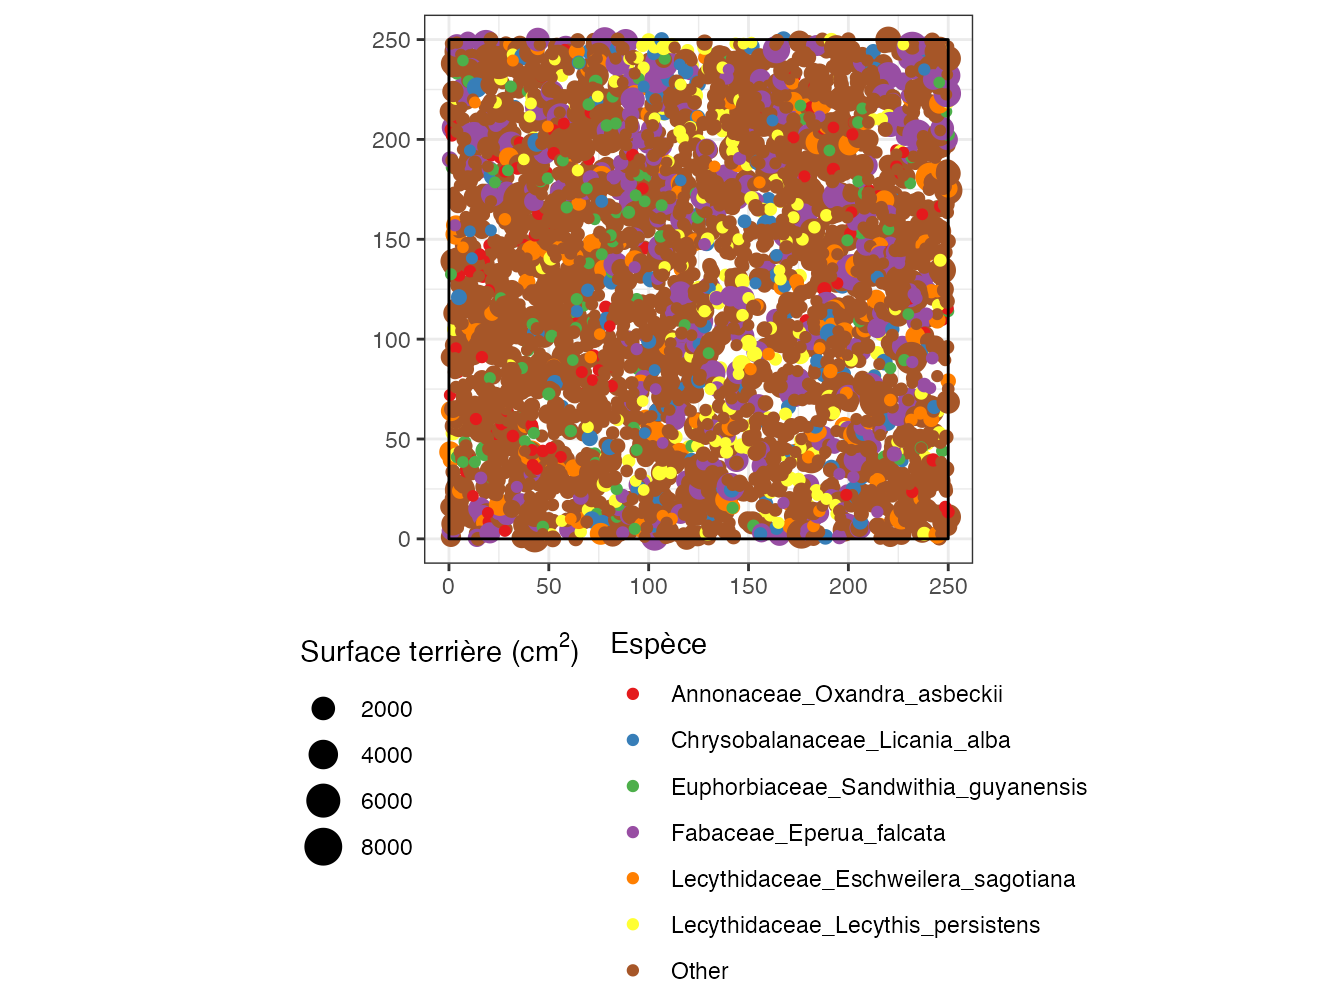
\includegraphics[width=\widthw]{MesuresBD_files/figure-latex/Paracou6MapFig-1} \end{minipage}}\needspace{\ht0+\dp0+2\baselineskip}\definesHSpace\hspace{-\rf}\box0\caption{Carte de la parcelle 6 de Paracou. Les points représentent les arbres. Leur taille est proportionnelle à leur surface terrière. Seules les espèces les plus fréquentes sont identifiées sur la carte.}\label{fig:Paracou6MapFig}
\end{figure}

\normalsize

Le code R pour réaliser la figure est le suivant:

\scriptsize

\begin{Shaded}
\begin{Highlighting}[]
\FunctionTok{library}\NormalTok{(}\StringTok{"divent"}\NormalTok{)}
\NormalTok{paracou\_6\_wmppp }\SpecialCharTok{\%\textgreater{}\%} 
\FunctionTok{autoplot}\NormalTok{(}
  \AttributeTok{labelSize =} \FunctionTok{expression}\NormalTok{(}\FunctionTok{paste}\NormalTok{(}\StringTok{"Surface terrière ("}\NormalTok{, cm}\SpecialCharTok{\^{}}\DecValTok{2}\NormalTok{, }\StringTok{")"}\NormalTok{)), }
  \AttributeTok{labelColor =} \StringTok{"Espèce"}
\NormalTok{) }\SpecialCharTok{+}
\FunctionTok{theme}\NormalTok{(}\AttributeTok{legend.position =} \StringTok{"bottom"}\NormalTok{, }\AttributeTok{legend.direction =} \StringTok{"vertical"}\NormalTok{, }\AttributeTok{legend.margin=}\FunctionTok{margin}\NormalTok{())}
\end{Highlighting}
\end{Shaded}

\normalsize

\hypertarget{notations}{%
\chapter*{Notations}\label{notations}}
\addcontentsline{toc}{chapter}{Notations}

Les notations mathématiques peuvent différer de celles de la littérature citée pour l'homogénéité de ce document.

Les matrices sont notées en caractères gras et majuscules: \(\mathbf{X}\).
Les éléments de la matrice \(\mathbf{X}\) sont notés \(x_{i,j}\).

Les vecteurs sont notés en gras minuscule: \(\mathbf{p}\).
Les nombres sont notés en minuscules, \(n\), et les variables aléatoires en majuscules: \(N\).
Les valeurs maximales des énumérations font exception: elles sont notées en majuscules pour les distinguer des indices: \(\sum_{s=1}^{S}{p_s}=1\).

Le produit matriciel de \(\mathbf{X}\) et \(\mathbf{Y}\) est noté \(\mathbf{X}\mathbf{Y}\). Dans les scripts R, l'opérateur est \texttt{\%*\%}.
Le produit de Hadamard (terme à terme) est noté \(\mathbf{X}\circ\mathbf{Y}\) (opérateur \texttt{*} dans R).
De même \(\mathbf{X}^n\) indique la puissance \(n\) au sens du produit matriciel d'une matrice carrée (opérateur \texttt{\%\^{}\%} du package \emph{expm}), alors que \(\mathbf{X}^{\circ n}\) est la matrice dont chaque terme est celui de \(\mathbf{X}\) à la puissance \(n\) (opérateur \texttt{\^{}} de R).
La matrice transposée de \(\mathbf{X}\) est notée \(\mathbf{X'}\).

Les notations sont les suivantes:

\noindent \({\mathbf 1}(\cdot)\): la fonction indicatrice, qui vaut 1 si la condition dans la parenthèse est vraie, 0 sinon.

\noindent \(\mathbf{1}_s\): le vecteur de longueur \(s\) composé uniquement de 1. \(\mathbf{1}_s\mathbf{1}_s'=\mathbf{J}_s\) où \(\mathbf{J}_s\) est la matrice carré de taille \(s\) ne contenant que des 1.

\noindent \(A\): l'aire d'étude, et, selon le contexte, sa surface.

\noindent \(C\): le taux de couverture de l'échantillon, c'est-à-dire la probabilité qu'un individu de la communauté appartienne à une des espèces échantillonnées.
\(C^{n}\) est le taux de couverture correspondant à un échantillon de taille \(n\).

\noindent \(^{q}\!D\): la diversité vraie (nombre de Hill pour les diversités \(\alpha\) et \(\gamma\)), nombre équivalent de communautés pour la diversité \(\beta\).
\(^{q}_{i}\!D_{\alpha}\) est la diversité \(\alpha\) mesurée dans la communauté \(i\).
\(^{q}\!\bar{D}\left(T\right)\) est la diversité phylogénétique.

\noindent \(\boldsymbol{\Delta}\): la matrice de dissimilarité dont les éléments sont \(\delta_{s,t}\), la dissimilarité entre l'espèce \(s\) et l'espèce \(t\).

\noindent \({\mathbb E}\left(X\right)\): l'espérance de la variable aléatoire \(X\).

\noindent \(f_{\nu}\): le nombre d'espèces observées \(\nu\) fois dans un échantillon (qui peut être défini par sa surface ou son nombre d'individus).
\(f_{>0}\) est le nombre d'espèces observées au moins une fois.
\(f_1\) s'appelle le nombre de \emph{singletons} et \(f_2\) le nombre de \emph{doubletons.}

\noindent \(^{q}\!H\): l'entropie de Tsallis (ou HCDT).
\(^{q}_{i}\!H_{\alpha}\) est l'entropie \(\alpha\) mesurée dans la communauté \(i\).
Si nécessaire, le vecteur des probabilités servant au calcul est précisé sous la forme \(^{q}\!H(\mathbf{p})\).
\(^{q}\!\bar{H}(T)\) est l'entropie phylogénétique.

\noindent \(I\): le nombre de communautés qui constituent une partition de la méta-communauté dans le cadre de la décomposition de la diversité.
Les communautés sont indexées par \(i\).

\noindent \(I(p_s)\): l'information apportée par l'observation d'un évènement de probabilité \(p_s\).
\(I(q_s,p_s)\) est le gain d'information apporté par l'expérience (\(q_s\) est observé) par rapport aux probabilités \(p_s\) attendues.

\noindent \(\mathbf{I}_s\): la matrice identité de rang \(s\): matrice carrée de taille \(s\times s\) dont la diagonale ne comporte que des 1 et les autres éléments sont nuls.

\noindent \(N\): le nombre (aléatoire) d'individus se trouvant dans l'aire d'étude.
\(N_s\) est la même variable aléatoire, mais restreinte aux individus de l'espèce \(s\).

\noindent \(n\): le nombre d'individus échantillonnés.
\(n_{s,i}\) est le nombre d'individus de l'espèce \(s\) dans la communauté \(i\).
Les effectifs totaux sont \(n_{s+}\) (pour l'espèce \(s\)), \(n_{+i}\) pour la communauté \(i\) et \(n\) le total général.
S'il n'y a qu'une communauté, le nombre d'individus par espèce est \(n_s\).

\noindent \(p_s\): la probabilité qu'un individu tiré au hasard appartienne à l'espèce \(s\), autrement dit la probabilité de l'espèce \(s\).
Son estimateur le plus simple, \({\hat{p}}_s\) est la fréquence observée.
Selon le contexte, \({\hat{p}}_s\) peut désigner un estimateur plus élaboré.
\(p_{s|i}\) est la même probabilité dans la communauté \(i\).
\(p_{\nu}\) est la probabilité d'une espèce observées \(\nu\) fois dans un échantillon.

\noindent \(\mathbf{p}=\left( p_1, p_2, \dots, p_s, \dots, p_S \right)\): le vecteur décrivant la distribution des probabilités \(p_s\), appelé simplexe en référence à sa représentation dans l'espace à \(S\) dimensions.

\noindent \({\pi}_{\nu}\): la probabilité qu'une espèce choisie au hasard soit représentée par \(\nu\) individus, \(\sum^n_{\nu=1}{{\pi}_{\nu}}\)=1.
Si l'espèce est choisie explicitement, la probabilité est notée \({\pi}_{n_s}\).

\noindent \(^{q}\!R\): l'entropie de Rényi d'ordre \(q\).

\noindent \(S\): le nombre d'espèces d'une communauté, considéré comme une variable aléatoire, estimé par \(\hat{S}\).

\noindent \(S(A)\) et \(S(n)\): le nombre d'espèces, considéré comme une fonction de la taille de l'échantillon.

\noindent \(t^{n}_{1-\alpha/2}\): le quantile d'une loi de Student à \(n\) degrés de liberté au seuil de risque \(\alpha\), classiquement 1,96 pour \(n\) grand et \(\alpha=5\%\).

\noindent \(\mathbf{Z}\): la matrice de similarité entre espèces dont les éléments sont \(z_{s,t}\), la similarité entre l'espèce \(s\) et l'espèce \(t\).

\noindent \(\mathrm{\Gamma}(\cdot)\): la fonction gamma.

\noindent \(\mathrm{\Psi}(\cdot)\): la fonction digamma.

\noindent \(\binom{n}{k}\): le nombre de combinaisons de \(k\) éléments parmi \(n\): \[\binom{n}{k}=\frac{n!}{k!\,(n-k)!}\].

\mainmatter

\hypertarget{part-notions}{%
\part{Notions}\label{part-notions}}

\hypertarget{chap-Notions}{%
\chapter{Notions de Diversité}\label{chap-Notions}}

\hypertarget{composantes}{%
\section{Composantes}\label{composantes}}



\scriptsize

\begin{SCfigure}

{\centering 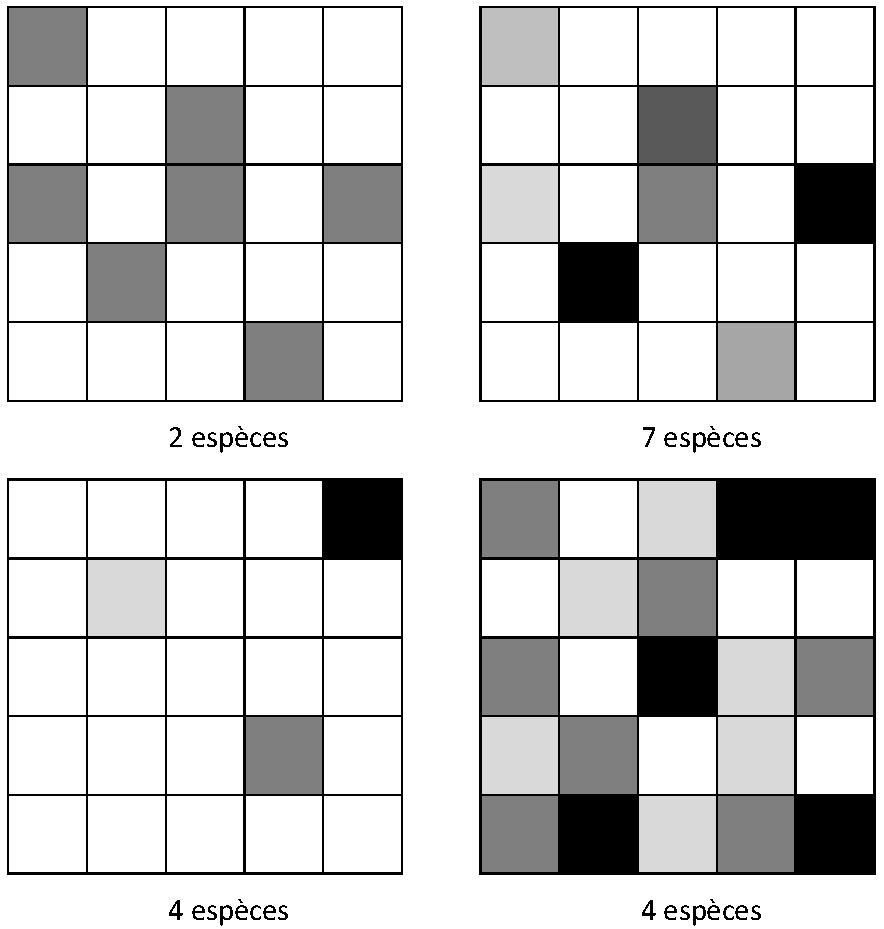
\includegraphics[width=0.8\linewidth]{images/Composantes} 

}

\caption{Importance de la richesse (en haut) et de l'équitabilité (en bas) pour la définition de la diversité. Ligne du haut: toutes choses égales par ailleurs, une communauté de 7 espèces semble plus diverse qu'une communauté de 2 espèces. Ligne du bas: à richesse égale, une communauté moins équitable (à gauche) semble moins diverse. Colonne de gauche: une communauté moins riche (en haut) peut sembler plus diverse si elle est plus équitable. Colonne de droite: idem pour la communauté du bas.}\label{fig:Composantes}
\end{SCfigure}

\normalsize

Une communauté comprenant beaucoup d'espèces mais avec une espèce dominante n'est pas perçue intuitivement comme plus diverse qu'une communauté avec moins d'espèces, mais dont les effectifs sont proches (figure \ref{fig:Composantes}, colonne de gauche).
La prise en compte de deux composantes de la diversité, appelées richesse et équitabilité, est nécessaire \autocite{Whittaker1965}.

\hypertarget{richesse}{%
\subsection{Richesse}\label{richesse}}

La richesse \autocite[terme introduit par][]{Mcintosh1967} est le nombre (ou une fonction croissante du nombre) de classes différentes présentes dans le système étudié, par exemple le nombre d'espèces d'arbres dans une forêt.

Un certain nombre d'hypothèses sont assumées plus ou moins explicitement:

\begin{itemize}
\tightlist
\item
  Les classes sont bien connues: compter le nombre d'espèces a peu de sens si la taxonomie n'est pas bien établie.
  C'est parfois une difficulté majeure quand on travaille sur les micro-organismes;
\item
  Les classes sont équidistantes: la richesse augmente d'une unité quand on rajoute une espèce, que cette espèce soit proche des précédentes ou extrêmement originale.
\end{itemize}

L'indice de richesse le plus simple et le plus utilisé est tout simplement le nombre d'espèces \(S\).

\hypertarget{uxe9quitabilituxe9}{%
\subsection{Équitabilité}\label{uxe9quitabilituxe9}}

La régularité de la distribution des espèces (équitabilité en Français, \emph{evenness} ou \emph{equitability} en anglais) est un élément important de la diversité.
Une espèce représentée abondamment ou par un seul individu n'apporte pas la même contribution à l'écosystème.
Sur la figure \ref{fig:Composantes}, la ligne du bas présente deux communautés de 4 espèces, mais celle de droite est beaucoup plus équitable de celle de gauche et semble intuitivement plus diverse.
À nombre d'espèces égal, la présence d'espèces très dominantes entraîne mathématiquement la rareté de certaines autres: on comprend donc assez intuitivement que le maximum de diversité sera atteint quand les espèces auront une répartition très régulière.

Un indice d'équitabilité est indépendant du nombre d'espèces (donc de la richesse).

La plupart des mesures de diversité courantes, comme celle de Simpson ou de Shannon, évaluent à la fois la richesse et l'équitabilité.

\hypertarget{disparituxe9}{%
\subsection{Disparité}\label{disparituxe9}}

Les mesures classiques de la diversité, dites mesures de diversité neutre (\emph{species-neutral diversity}) ou taxonomique ne prennent pas en compte une quelconque distance entre classes.
Pourtant, deux espèces du même genre sont de toute évidence plus proches que deux espèces de familles différentes.
Les mesures de diversité non neutres (chapitre \ref{chap-cadrephyfonc}) prennent en compte cette notion, qui nécessite quelques définitions supplémentaires \autocite{Mouillot2005,Ricotta2007}.

La mesure de la différence entre deux classes est souvent une distance, mais parfois une mesure qui n'a pas toutes les propriétés d'une distance: une dissimilarité.
Les mesures de \emph{divergence} \autocite{Pavoine2011} sont construites à partir de la dissimilarité entre les classes, avec ou sans pondération par la fréquence.

Si la divergence entre espèces est une distance évolutive comme l'âge du plus récent ancêtre commun, la diversité sera dite phylogénétique.
Si c'est une distance fonctionnelle, définie par exemple dans l'espace des traits fonctionnels, la diversité sera dite fonctionnelle.

La disparité \autocite{Runnegar1987}, divergence moyenne entre deux espèces (indépendamment des fréquences), ou de façon équivalente la longueur totale des branches d'un arbre phylogénétique, est la composante qui décrit à quel point les espèces sont différentes les unes des autres.

Les mesures de \emph{régularité} décrivent la façon dont les espèces occupent l'espace des niches (régularité fonctionnelle) ou la régularité dans le temps et entre les clades des évènements de spéciation représentés par un arbre phylogénétique.
Ce concept complète celui d'équitabilité dans les mesures classiques: la diversité augmente avec la richesse, la divergence entre espèces, et la régularité (qui se réduit à l'équitabilité quand toutes les espèces sont également divergentes entre elles).

\hypertarget{agruxe9gation}{%
\subsection{Agrégation}\label{agruxe9gation}}

À partir d'une large revue de la littérature dans plusieurs disciplines scientifiques s'intéressant à la diversité (au-delà de la biodiversité), \textcite{Stirling2007} estime que les trois composantes, qu'il nomme \emph{variété} (richesse), \emph{équilibre} (équitabilité) et \emph{disparité}, recouvrent tous les aspects de la diversité.

Stirling définit la propriété d'\emph{agrégation} comme la capacité d'une mesure de diversité à combiner explicitement les trois composantes précédentes.
Cela ne signifie pas que les composantes contribuent indépendamment les unes des autres à la diversité \autocite{Jost2010}.

\hypertarget{niveaux-de-luxe9tude}{%
\section{Niveaux de l'étude}\label{niveaux-de-luxe9tude}}

La diversité est classiquement estimée à plusieurs niveaux emboîtés, nommés \(\alpha\), \(\beta\) et \(\gamma\) par \textcite[page 320]{Whittaker1960} qui a nommé \(\alpha\) la diversité locale qu'il mesurait avec l'indice \(\alpha\) de Fisher (voir le chapitre \ref{chap-Fisher}) et a utilisé les lettres suivantes selon ses besoins.

\hypertarget{diversituxe9-alpha-beta-et-gamma}{%
\subsection{\texorpdfstring{Diversité \(\alpha\), \(\beta\) et \(\gamma\)}{Diversité \textbackslash alpha, \textbackslash beta et \textbackslash gamma}}\label{diversituxe9-alpha-beta-et-gamma}}

La diversité \(\alpha\) est la diversité locale, mesurée à l'intérieur d'un système délimité.
Plus précisément, il s'agit de la diversité dans un habitat uniforme de taille fixe.



\scriptsize

\begin{SCfigure}

{\centering 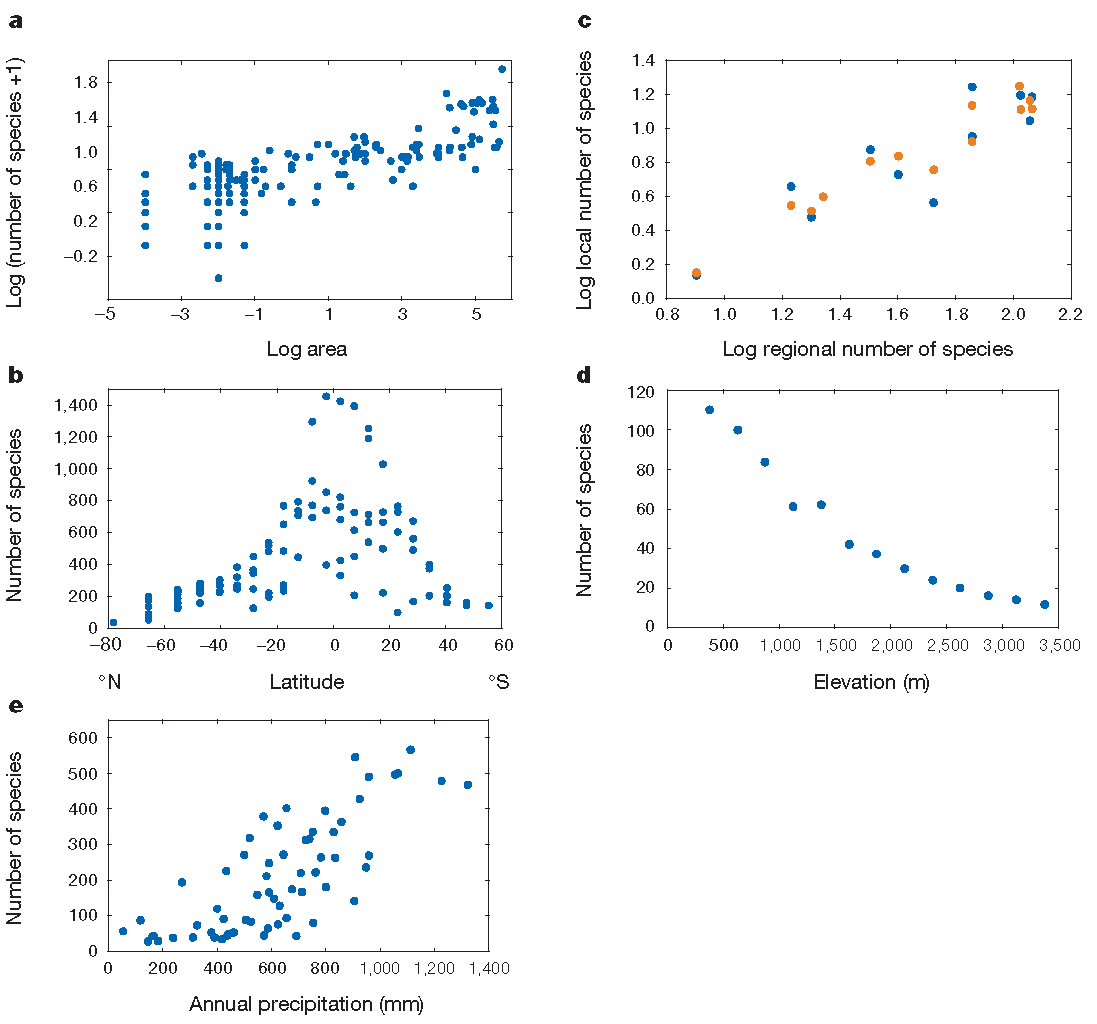
\includegraphics[width=1\linewidth]{images/Gaston2000} 

}

\caption{Patrons de biodiversité. (a) Le nombre d'espèces de vers de terre augmente en fonction de la surface échantillonnée, de 100 m² à plus de 500000 km² selon la relation d'Arrhenius). (b) Nombre d'espèces d'oiseaux en fonction de la latitude. (c) Relation entre la richesse régionale et la richesse locale. (d) Nombre d'espèces de chauves-souris en fonction de l'altitude dans une réserve au Pérou. (e) Nombre d'espèces de végétaux ligneux en fonction des précipitations en Afrique du Sud.}\label{fig:Gaston2000}
\end{SCfigure}

\normalsize

De façon générale \autocite{Gaston2000}, la richesse spécifique diminue avec la latitude (la diversité est plus grande dans les zones tropicales, et au sein de celles-ci, quand on se rapproche de l'équateur), voir figure \ref{fig:Gaston2000} \autocite[figure 1]{Gaston2000}.
La tendance est la même pour la diversité génétique intraspécifique \autocite{Miraldo2016}.
La richesse diminue avec l'altitude.
Elle est généralement plus faible sur les îles, où elle décroît avec la distance au continent, source de migrations.

La diversité \(\beta\) mesure à quel point les systèmes locaux sont différents.
Cette définition assez vague a fait l'objet de nombreux débats \autocite{Moreno2010}.

Enfin, la diversité \(\gamma\) est similaire à la diversité \(\alpha\), prise en compte sur l'ensemble du système étudié.
Les diversités \(\alpha\) et \(\gamma\) se mesurent donc de la même façon, mais à différentes échelles.

\hypertarget{duxe9composition}{%
\subsection{Décomposition}\label{duxe9composition}}

\textcite{Whittaker1977} a proposé sans succès une normalisation des échelles d'évaluation de la biodiversité, en introduisant la diversité régionale \(\varepsilon\) (\(\gamma\) étant réservé au paysage et \(\alpha\) à l'habitat) et la diversité \(\delta\) entre les paysages.
Seuls les trois niveaux originaux ont été conservés par la littérature, sans définition stricte des échelles d'observation.

La distinction entre les diversités \(\alpha\) et \(\beta\) dépend de la finesse de la définition de l'habitat.
La distinction de nombreux habitats diminue la diversité \(\alpha\) au profit de la \(\beta\).
Il est donc important de définir une mesure qui ne dépende pas de ce découpage, donc une mesure cumulative (additive ou multiplicative) décrivant la diversité totale, décomposable en la somme ou le produit convenablement pondérés de toutes les diversités \(\alpha\) des habitats (diversité intra) et de la diversité \(\beta\) inter-habitat.

Nous appellerons \emph{communauté} le niveau de découpage concernant la diversité \(\alpha\) et \emph{méta-communauté} le niveau de regroupement pour l'estimation de la diversité \(\gamma\).

\hypertarget{courbes-daccumulation}{%
\section{Courbes d'accumulation}\label{courbes-daccumulation}}



\scriptsize

\begin{SCfigure}

{\centering 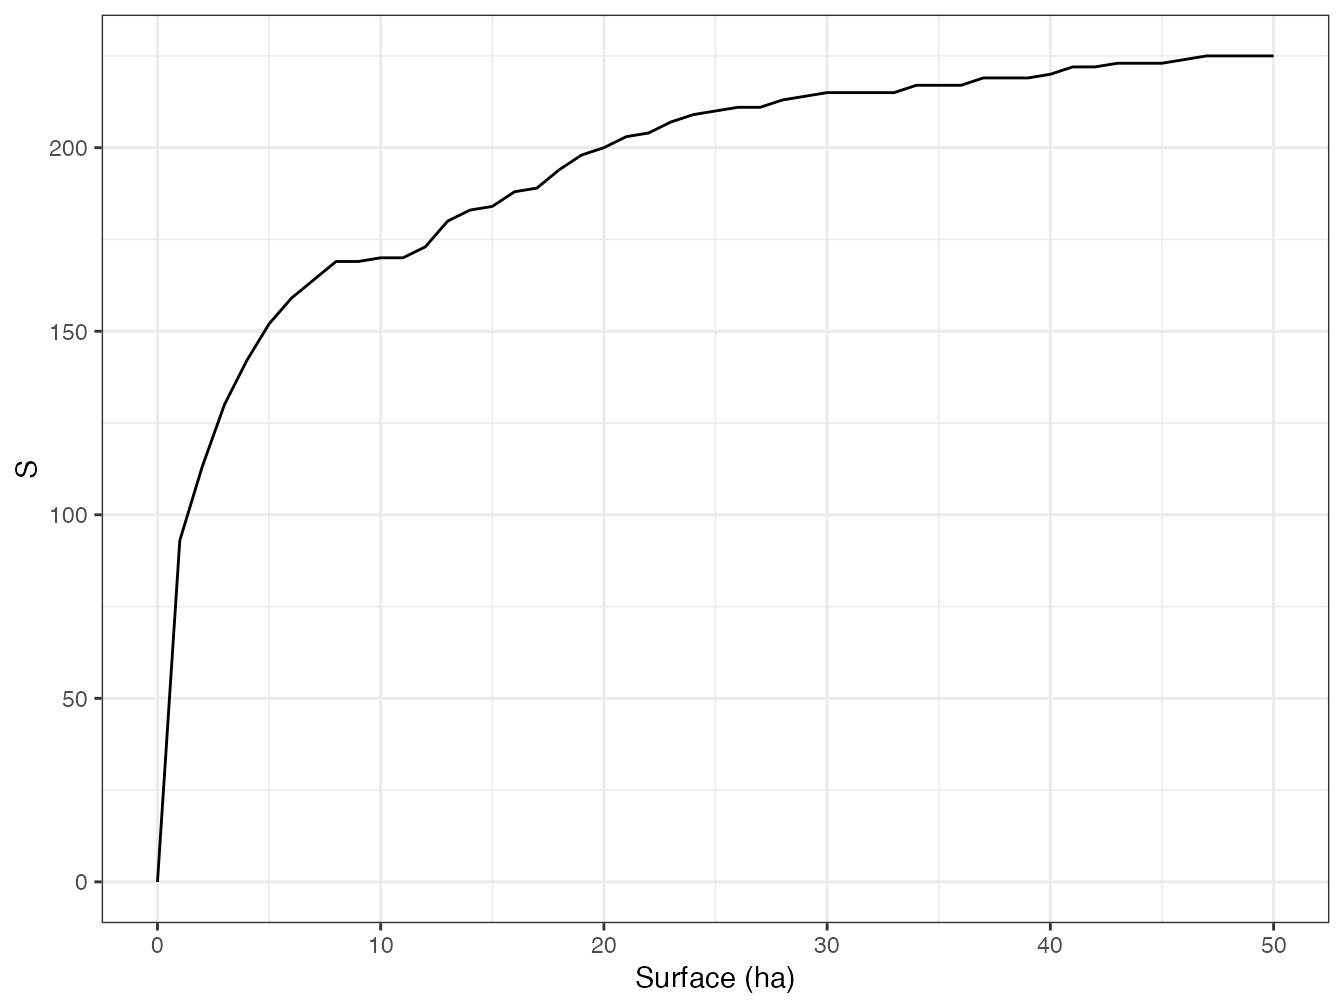
\includegraphics[width=0.8\linewidth]{MesuresBD_files/figure-latex/SACFig-1} 

}

\caption{Courbe d'accumulation des espèces d'arbres du dispositif de Barro Colorado Island. Le nombre d'espèces est cumulé dans l'ordre des carrés d'un hectare du dispositif.}\label{fig:SACFig}
\end{SCfigure}

\normalsize

Evaluer la diversité d'une communauté nécessite en pratique de l'inventorier.
Le nombre d'espèces découvertes en fonction de l'effort d'échantillonnage permet de tracer une courbe d'accumulation (SAC: \emph{Species Acumulation Curve}).
Une courbe de raréfaction (\emph{Rarefaction Curve}) peut être calculée en réduisant par des outils statistiques l'effort d'échantillonnage réel pour obtenir une SAC théorique, libérée des aléas de l'ordre de prise en compte des données.

La figure \ref{fig:SACFig} montre l'accumulation des espèces pour les données de BCI.
Une SAC peut être tracée en fonction de la surface, du nombre d'individus ou du nombres de placettes d'échantillonnage, selon les besoins.

Code R pour réaliser la figure \ref{fig:SACFig}:

\scriptsize

\begin{Shaded}
\begin{Highlighting}[]
\FunctionTok{library}\NormalTok{(}\StringTok{"vegan"}\NormalTok{)}
\FunctionTok{data}\NormalTok{(BCI)}
\CommentTok{\# Chaque parcelle (ligne) cumule ses abondances à la précédente}
\NormalTok{cumul }\OtherTok{\textless{}{-}} \FunctionTok{apply}\NormalTok{(BCI, }\DecValTok{2}\NormalTok{, cumsum)}
\CommentTok{\# Le nombre d\textquotesingle{}espèces de chaque parcelle est cumulé }
\NormalTok{Richesse }\OtherTok{\textless{}{-}} \FunctionTok{apply}\NormalTok{(cumul, }\DecValTok{1}\NormalTok{, }\ControlFlowTok{function}\NormalTok{(x) }\FunctionTok{sum}\NormalTok{(x }\SpecialCharTok{\textgreater{}} \DecValTok{0}\NormalTok{))}
\FunctionTok{ggplot}\NormalTok{(}
  \FunctionTok{data.frame}\NormalTok{(}
    \AttributeTok{A =} \DecValTok{0}\SpecialCharTok{:}\DecValTok{50}\NormalTok{, }
    \AttributeTok{S =} \FunctionTok{c}\NormalTok{(}\DecValTok{0}\NormalTok{, Richesse)}
\NormalTok{  )}
\NormalTok{) }\SpecialCharTok{+}
  \FunctionTok{geom\_line}\NormalTok{(}\FunctionTok{aes}\NormalTok{(}\AttributeTok{x =}\NormalTok{ A, }\AttributeTok{y =}\NormalTok{ S)) }\SpecialCharTok{+}
  \FunctionTok{labs}\NormalTok{(}\AttributeTok{x =} \StringTok{"Surface (ha)"}\NormalTok{)}
\end{Highlighting}
\end{Shaded}

\normalsize

Les courbes d'accumulation peuvent aussi concerner la diversité (voir le chapitre \ref{chap-Accumulation}), mesurée au-delà du nombre d'espèces.

Plus généralement, une courbe aire-espèces (SAR: \emph{Species Area Relationship}) représente le nombre d'espèces observées en fonction de la surface échantillonnée (figure \ref{fig:Williamson2001}).
Il existe plusieurs façons de prendre en compte cette relation \autocite{Scheiner2003}, classables en deux grandes familles \autocite{Dengler2009}:

\begin{itemize}
\tightlist
\item
  Dans une SAR au sens strict, chaque point représente une communauté.
  La question traitée est la relation entre le nombre d'espèces et la taille de chaque communauté, en lien avec des processus écologiques;
\item
  Une courbe d'accumulation (SAC) ne représente que l'effet statistique de l'échantillonnage.
  Pour éviter toute confusion, le terme SAR ne doit pas être utilisé pour décrire une SAC.
\end{itemize}

\hypertarget{diversituxe9-asymptotique}{%
\section{Diversité asymptotique}\label{diversituxe9-asymptotique}}

Augmenter l'effort d'échantillonnage peut permettre d'atteindre un stade où la diversité n'augmente plus: sa valeur est appelée \emph{diversité asymptotique}.
Dans des communautés très diverses comme les forêts tropicales, la diversité asymptotique ne peut en général pas être observée sur le terrain à cause de la variabilité de l'environnement: l'augmentation de la surface inventoriée amène à échantillonner dans des communautés différentes avant d'atteindre la diversité asymptotique de la communauté étudiée.
La diversité asymptotique est donc celle d'une communauté théorique qui n'existe généralement pas.
En d'autres termes, c'est la diversité d'une communauté dont l'inventaire disponible serait un échantillon représentatif.

Evaluer la diversité asymptotique nécessite d'utiliser des estimateurs de diversité, dont la précision dépend de l'exhaustivité de l'échantillonnage.
La diversité peut aussi être estimée pour un effort donné: un hectare de forêt ou 5000 arbres par exemple, ou encore un taux de couverture choisi, qui décrit mieux la qualité de l'échantillonnage.

\hypertarget{sec-Couverture}{%
\section{Couverture}\label{sec-Couverture}}

Le taux de couverture (\emph{sample coverage}) de l'échantillon est la proportion des espèces découvertes,
\begin{equation}
  \label{eq:C}
  C = \sum^S_{s=1}{{\mathbf 1}\left( n_s > 0 \right) p_s},
\end{equation}

où \({\mathbf 1}(\cdot)\) est la fonction indicatrice.
Son complément à 1 est appelé déficit de couverture (\emph{coverage deficit}).

Le déficit de couverture est la probabilité qu'un individu tiré au hasard dans la communauté appartienne à une espèce absente de l'échantillon inventorié.
C'est donc aussi la probabilité qu'un individu ajouté à l'inventaire lui ajoute une nouvelle espèce \autocite{Good1953}.
La pente de la courbe d'accumulation donnant l'espérance du nombre d'espèces en fonction du nombre d'individus (courbe de raréfaction de la figure \ref{fig:Gotelli2001}) est donc égale au déficit de couverture \autocite{Chao2012b}:

\begin{equation}
  \label{eq:DefC}
  1 - {\mathbb E}\left[ C\left( n \right) \right] = {\mathbb E}\left[ S\left( n + 1 \right) \right] - {\mathbb E}\left[ S\left( n \right) \right],
\end{equation}

où \(C(n)\) est le taux de couverture d'un échantillon de taille \(n\) et \(S(n)\) le nombre d'espèces découvertes dans cet échantillon.

Le taux de couverture augmente avec l'effort d'échantillonnage.
Plus il est élevé, meilleures seront les estimations de la diversité: la diversité asymptotique est obtenue quand il atteint 1.
Les estimateurs de la diversité asymptotique développés plus loin reposent largement sur cette notion pour la correction du biais d'échantillonnage \autocite{Dauby2012}, c'est-à-dire la sous-estimation systématique de la diversité due aux espèces non observées, qui est un des éléments du biais d'estimation.

Pour comparer la diversité non asymptotique de deux communautés avec le même effort d'échantillonnage, \textcite{Chao2012b} montrent que le taux de couverture plutôt que la taille de l'échantillon doit être identique.

\hypertarget{formule-des-fruxe9quences-de-good-turing}{%
\subsection{Formule des fréquences de Good-Turing}\label{formule-des-fruxe9quences-de-good-turing}}

La relation fondamentale entre les fréquences des espèces dans un échantillon est due à Turing et a été publiée par \textcite{Good1953}.
En absence de toute information sur la loi de distribution des espèces, en supposant seulement que les individus sont tirés indépendamment les uns des autres selon une loi multinomiale respectant ces probabilités, la formule de Good-Turing relie la probabilité attendue \({\mathbb E}(p_\nu)\) d'une espèce représentée par \(\nu\) individus au rapport entre les nombres d'espèces représentées \(\nu+1\) fois et \(\nu\) fois:

\begin{equation}
  \label{eq:alphanu}
  {\mathbb E}\left( p_\nu \right) 
  \approx \frac{(\nu + 1)}{n} \frac{{\mathbb E}\left( f_{\nu+1} \right)}{{\mathbb E}\left( f_\nu \right)}.
\end{equation}

La variance de \(p_\nu\) est connue:

\begin{equation}
  \label{eq:varpnu}
  \operatorname{Var}\left( p_\nu \right) 
  \approx {\mathbb E}\left( p_\nu \right) \left[ {\mathbb E}\left( p_{\nu + 1} \right) - {\mathbb E}\left( p_\nu \right) \right].
\end{equation}

Elle est petite en comparaison de l'espérance.

Le nombres d'espèces observées \(\nu\) et \(\nu + 1\) fois varient selon l'échantillonnage.
La relation de Good-Turing concerne leur espérance mais comme on ne dispose en général que d'un seul inventaire, les espérances \({\mathbb E}(f_\nu)\) et \({\mathbb E}(f_{\nu + 1})\) sont remplacées par les valeurs observées.
De même, chacune des espèces observées \(\nu\) fois a une probabilité différente: la relation ne permet pas de prédire précisément, pour un échantillon, les probabilités de chaque espèce.

Ces relations sont le fondement de plusieurs estimateurs de biodiversité présentés plus loin.
Les singletons (\(f_{1}\): le nombre d'espèces observées une seule fois) et les doubletons (\(f_{2}\): le nombre d'espèces observées deux fois) ont une importance centrale.
Pour \(\nu=1\), on a par exemple \(\alpha_1 = 2 f_{2}/(nf_{1})\): la fréquence d'une espèce typiquement représentée par un singleton est proportionnelle au rapport entre le nombre des doubletons et des singletons.
Cet estimateur de probabilité est meilleur que l'estimateur naïf \(1/n\): en d'autres termes, la distribution des fréquences observées permet d'estimer les probabilités de façon non triviale.

La relation a été précisée \autocite[eq. 6 et 7a]{Chiu2014a} en limitant les approximations dans les calculs.
La seule approximation nécessaire est que les probabilités des espèces représentées le même nombre de fois \(\nu\) varient peu et puissent être considérées toutes égales à \({\mathbb E}(p_\nu)\), ce qui est acceptable puisque la variance de \(p_\nu\) est petite.
On peut alors estimer directement
\begin{equation}
  \label{eq:GoodTuring2014}
   \hat{p_\nu} 
   = \frac{\left( \nu + 1 \right) f_{\nu + 1}}{\left(n - \nu \right) f_{\nu} + \left(\nu + 1 \right) f_{\nu + 1}}
\end{equation}

en remplaçant les espérances par les valeurs observées.

Ce nouvel estimateur est à la base de l'estimateur de Chao amélioré et des estimateurs d'entropie de Chao et Jost (sections \ref{sec-BiaisShannon} et \ref{sec-BiaisHCDT}).

\hypertarget{estimation-du-taux-de-couverture}{%
\subsection{Estimation du taux de couverture}\label{estimation-du-taux-de-couverture}}

En posant \(\nu=0\) dans l'équation \eqref{eq:alphanu}, \({\mathbb E}(p_0) \times f_{0} = \pi_0\), la probabilité totale des espèces non représentées, vaut approximativement \(f_{1}/n\).
C'est l'estimateur de Good ou Good-Turing, parfois appelé abusivement \enquote{formule de Turing} \autocite{Zhang2007}:

\begin{equation}
  \label{eq:CGood}
  \hat{C} = 1 - \frac{f_1}{n}.
\end{equation}

Cet estimateur est biaisé \autocite{Zhang2007}. En réalité,
\begin{equation}
  \label{eq:CsansBiais}
  C = 1 - \frac{{\mathbb E}(f_1) - \pi_1}{n}.
\end{equation}

L'estimateur de Good néglige le terme \(\pi_1\), la somme des probabilités des espèces observées une fois.
Ce terme peut être estimé avec un biais plus petit.
\textcite{Chao1988} puis \textcite{Zhang2007} proposent l'estimateur suivant, qui utilise toute l'information disponible et a le plus petit biais possible:

\begin{equation}
  \label{eq:CZhang}
  \hat{C} = 1 - \sum^{n}_{\nu = 1}{\left( -1 \right)}^{\nu + 1}{\binom{n}{\nu}}^{-1}f_\nu.
\end{equation}

Les termes de la somme décroissent très vite avec \(\nu\).
En se limitant à \(\nu=1\), l'estimateur se réduit à celui de Good.

\textcite{Esty1983}, complété par \textcite{Zhang2009}, a montré que l'estimateur était asymptotiquement normal et a calculé l'intervalle de confiance de \(\hat{C}\):

\begin{equation}
  \label{eq:hatC}
  C = \hat{C} \pm t^{n}_{1 - \alpha / 2} \frac{\sqrt{f_1 \left( 1 - \frac{f_{1}}{n} \right) + 2f_2}}{n}.
\end{equation}

Où \(t^{n}_{1 - \alpha / 2}\) est le quantile d'une loi de Student à \(n\) degrés de libertés au seuil de risque \(\alpha\), classiquement 1,96 pour \(n\) grand et \(\alpha = 5\%\).

Un autre estimateur est utilisé dans le logiciel SPADE \autocite{Chao2010a} et son portage sous R, le package \emph{spadeR} \autocite{Chao2016c}.
Il est la base des estimateurs d'entropie de Chao et Jost (section \ref{sec-BiaisHCDT}).
L'estimation de l'équation \eqref{eq:CsansBiais} donne la relation
\begin{equation}
  \label{eq:hatC2}
  \hat{C} = 1 - \frac{f_{1} - \hat{\pi}_1}{n}.
\end{equation}

Or, \(\hat{\pi}_1 = f_{1} \hat{p}_1\).
\(p_1\) peut être estimé par la relation de Good-Turing \eqref{eq:GoodTuring2014}, en remplaçant \(f_0\) par l'estimateur Chao1 \eqref{eq:Chao1}.
Alors:

\begin{equation} 
  \label{eq:CChao}
  \hat{C} 
  = 1 - \frac{f_1}{n}(1 - \hat{p}_1)
  = 1 - \frac{f_1}{n}\left[ \frac{\left( n - 1 \right) f_1}{\left( n - 1 \right) f_1 + 2f_2} \right].
\end{equation}

Dans le package \emph{divent}, la fonction \texttt{coverage} calcule les trois estimateurs (celui de Zhang et Huang par défaut):

\scriptsize

\begin{Shaded}
\begin{Highlighting}[]
\FunctionTok{library}\NormalTok{(}\StringTok{"divent"}\NormalTok{)}
\NormalTok{BCI }\SpecialCharTok{\%\textgreater{}\%} 
  \FunctionTok{colSums}\NormalTok{() }\SpecialCharTok{\%\textgreater{}\%} 
  \FunctionTok{coverage}\NormalTok{()}
\end{Highlighting}
\end{Shaded}

\begin{verbatim}
## # A tibble: 1 x 2
##   estimator  coverage
##   <chr>         <dbl>
## 1 ZhangHuang    0.999
\end{verbatim}

\normalsize

Le taux de couverture de BCI est proche de 1 parce que l'inventaire couvre 50~ha.
Il est moindre sur les 6.25~ha de la parcelle 6 de Paracou:

\scriptsize

\begin{Shaded}
\begin{Highlighting}[]
\NormalTok{paracou\_6\_abd }\SpecialCharTok{\%\textgreater{}\%} 
  \FunctionTok{colSums}\NormalTok{() }\SpecialCharTok{\%\textgreater{}\%} 
  \FunctionTok{coverage}\NormalTok{()}
\end{Highlighting}
\end{Shaded}

\begin{verbatim}
## # A tibble: 1 x 2
##   estimator  coverage
##   <chr>         <dbl>
## 1 ZhangHuang    0.972
\end{verbatim}

\normalsize

Les estimateurs présentés ici supposent une population de taille infinie (de façon équivalente, les individus sont tirés avec remise).
Le cas des populations de taille finie est traité par \textcite{Chao2012} et \textcite{Hwang2014}.

\hypertarget{compluxe9tude}{%
\subsection{Complétude}\label{compluxe9tude}}

La complétude de l'échantillonnage est la proportion du nombre d'espèces observées: \(f_{>0} / S\).
Elle compte simplement les espèces et ne doit pas être confondue avec la couverture qui somme leurs probabilités: le taux de complétude est toujours très inférieur au taux de couverture parce que les espèces non échantillonnées sont les plus rares.

La complétude du même échantillon d'arbres de forêt tropicale que dans l'exemple précédent peut être estimée en divisant le nombre d'espèces observées par le nombre d'espèces estimées (voir section \ref{sec-Richesse}).
À BCI:

\scriptsize

\begin{Shaded}
\begin{Highlighting}[]
\NormalTok{bci\_abd }\OtherTok{\textless{}{-}} \FunctionTok{colSums}\NormalTok{(BCI)}
\CommentTok{\# Espèces observées}
\NormalTok{(obs }\OtherTok{\textless{}{-}} \FunctionTok{div\_richness}\NormalTok{(bci\_abd, }\AttributeTok{estimator  =} \StringTok{"naive"}\NormalTok{))}
\end{Highlighting}
\end{Shaded}

\begin{verbatim}
## # A tibble: 1 x 3
##   estimator order diversity
##   <chr>     <dbl>     <int>
## 1 naive         0       225
\end{verbatim}

\begin{Shaded}
\begin{Highlighting}[]
\CommentTok{\# Richesse estimée}
\NormalTok{(est }\OtherTok{\textless{}{-}} \FunctionTok{div\_richness}\NormalTok{(bci\_abd))}
\end{Highlighting}
\end{Shaded}

\begin{verbatim}
## # A tibble: 1 x 3
##   estimator   order diversity
##   <chr>       <dbl>     <dbl>
## 1 Jackknife 1     0       244
\end{verbatim}

\begin{Shaded}
\begin{Highlighting}[]
\CommentTok{\# Complétude}
\NormalTok{obs}\SpecialCharTok{$}\NormalTok{diversity }\SpecialCharTok{/}\NormalTok{ est}\SpecialCharTok{$}\NormalTok{diversity}
\end{Highlighting}
\end{Shaded}

\begin{verbatim}
## [1] 0.9221311
\end{verbatim}

\normalsize

À Paracou:

\scriptsize

\begin{Shaded}
\begin{Highlighting}[]
\CommentTok{\# Espèces observées}
\NormalTok{(obs }\OtherTok{\textless{}{-}} \FunctionTok{div\_richness}\NormalTok{(}\FunctionTok{colSums}\NormalTok{(paracou\_6\_abd), }\AttributeTok{estimator  =} \StringTok{"naive"}\NormalTok{))}
\end{Highlighting}
\end{Shaded}

\begin{verbatim}
## # A tibble: 1 x 3
##   estimator order diversity
##   <chr>     <dbl>     <int>
## 1 naive         0       335
\end{verbatim}

\begin{Shaded}
\begin{Highlighting}[]
\CommentTok{\# Richesse estimée}
\NormalTok{(est }\OtherTok{\textless{}{-}} \FunctionTok{div\_richness}\NormalTok{(}\FunctionTok{colSums}\NormalTok{(paracou\_6\_abd)))}
\end{Highlighting}
\end{Shaded}

\begin{verbatim}
## # A tibble: 1 x 3
##   estimator   order diversity
##   <chr>       <dbl>     <dbl>
## 1 Jackknife 2     0       473
\end{verbatim}

\begin{Shaded}
\begin{Highlighting}[]
\CommentTok{\# Complétude}
\NormalTok{obs}\SpecialCharTok{$}\NormalTok{diversity }\SpecialCharTok{/}\NormalTok{ est}\SpecialCharTok{$}\NormalTok{diversity}
\end{Highlighting}
\end{Shaded}

\begin{verbatim}
## [1] 0.7082452
\end{verbatim}

\normalsize

\hypertarget{le-probluxe8me-de-lespuxe8ce}{%
\section{Le problème de l'espèce}\label{le-probluxe8me-de-lespuxe8ce}}

Évaluer la richesse spécifique suppose que les espèces soient définies clairement, ce qui n'est de toute évidence pas le cas \autocite{Casetta2014}.
Le premier aspect du problème concerne la nature des espèces: réalité naturelle ou seulement représentation simplificatrice.
Une analyse historique et philosophique en est faite par \textcite{Richards2010}.
L'autre aspect, avec des conséquences pratiques plus immédiates, concerne leur délimitation.
\textcite{Mayden1997} recense vingt-deux définitions différentes du concept d'espèce.
\textcite{Wilkins2011} estime qu'il n'y a qu'un seul concept d'espèce mais sept définitions, c'est-à-dire sept façons de les identifier, et vingt-sept variations ou mélanges de ces définitions.

La définition historique est celle de \emph{morphoespèce}, qui classe les espèces selon leurs formes, supposées d'abord immuables.
La définition moderne la plus répandue est celle d'espèce \emph{biologique} \autocite{Dobzhansky1937}: un \enquote{groupe de populations naturelles isolées reproductivement les unes des autres} \autocite{Mayr1942}.
Lorsque les populations d'une espèce sont isolées géographiquement, leur capacité à se reproduire ensemble est toute théorique (et rarement vérifiée expérimentalement).
Des populations allopatriques n'ont pas de flux de gènes réels entre elles et peuvent être considérées comme des espèces distinctes selon la définition d'espèce \emph{phylogénétique}: \enquote{le plus petit groupe identifiable d'individus avec un pattern commun d'ancêtres et de descendants} \autocite{Cracraft1983}.
C'est l'unité génétique détectée par la méthode du coalescent pour la délimitation des espèces \autocite{Sukumaran2017}.
Le nombre d'espèces phylogénétiques est bien supérieur au nombre d'espèces biologiques.
Enfin, \textcite{VanValen1976} définit les espèces par la niche écologique qu'elles occupent (à partir de l'exemple des chênes blancs européens) plutôt que par les flux de gènes (permanents entre les espèces distinctes): la définition \emph{écologique} d'espèce est proche du concept de complexe d'espèces \autocite[ensemble d'espèces voisines échangeant des gènes,][]{Pernes1984}.

Le choix de la définition modifie considérablement sur la quantification de la richesse \autocite{Agapow2004}.
Des problèmes méthodologiques s'ajoutent aux problèmes conceptuels \autocite{Hey2001}: la séparation ou le regroupement de plusieurs populations ou morphotypes en un nombre plus ou moins grand d'espèces est un choix qui reflète les connaissances du moment et peut évoluer \autocite{Barberousse2014}.

L'impact du problème de l'espèce sur la mesure de la diversité reste sans solution à ce stade, si ce n'est d'utiliser les mêmes définitions si des communautés différentes doivent être comparées.
L'approche phylogénétique (chapitre \ref{chap-Phyloentropie}) permet de contourner le problème: si deux taxons très semblables apportent à peine plus de diversité qu'un seul taxon, le choix de les distinguer ou non n'est pas critique.

\hypertarget{sec-SAD}{%
\chapter{Distribution de l'abondance des espèces (SAD)}\label{sec-SAD}}

La distribution de l'abondance des espèces (SAD: \emph{Species Abundance Distribution}) est la loi statistique qui donne l'abondance attendue de chaque espèce d'une communauté.
Les espèces ne sont pas identifiées individuellement, mais par le nombre d'individus leur appartenant.



\scriptsize

\begin{SCfigure}

{\centering 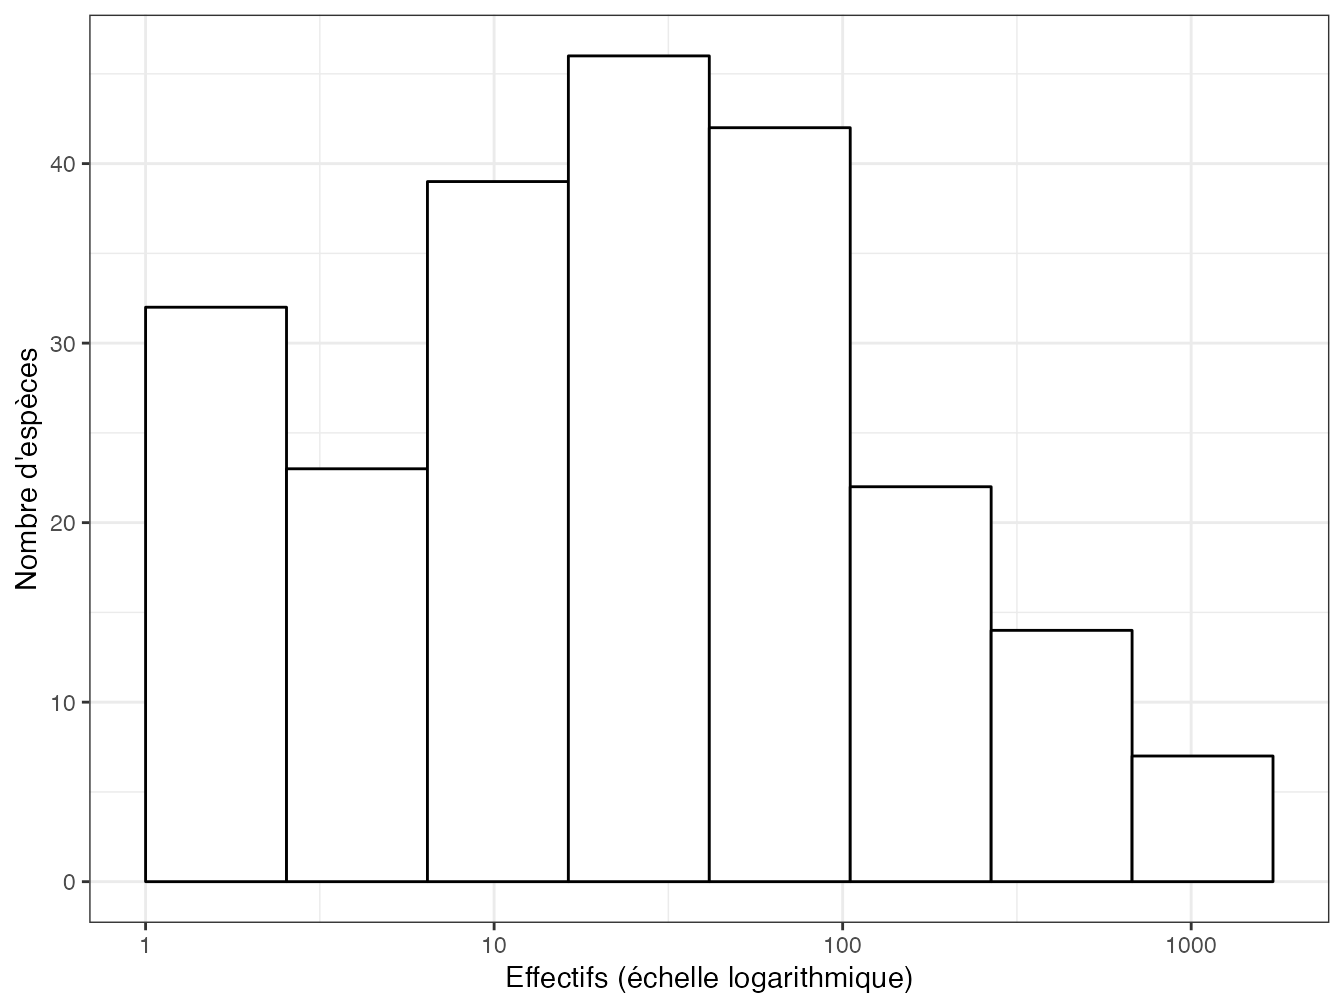
\includegraphics[width=0.8\linewidth]{MesuresBD_files/figure-latex/SADFig-1} 

}

\caption{Histogramme des fréquences (diagramme de Preston) des arbres du dispositif de Barro Colorado Island. En abscisse: le nombre d'arbres de chaque espèce (en logarithme); en ordonnée: le nombre d'espèces.}\label{fig:SADFig}
\end{SCfigure}

\normalsize

Elle peut être représentée sous la forme d'un histogramme des fréquences (diagramme de \textcite{Preston1948}, figure \ref{fig:SADFig}) ou bien d'un diagramme rang-abondance (RAC: \emph{Rank Abundance Curve} ou diagramme de \textcite{Whittaker1965}, figure \ref{fig:RACFig}).
Le RAC est souvent utilisé pour reconnaître des distributions connues.
\textcite{Izsak2012} ont étudié les propriétés des RAC pour les principales SAD.



\scriptsize

\begin{SCfigure}

{\centering 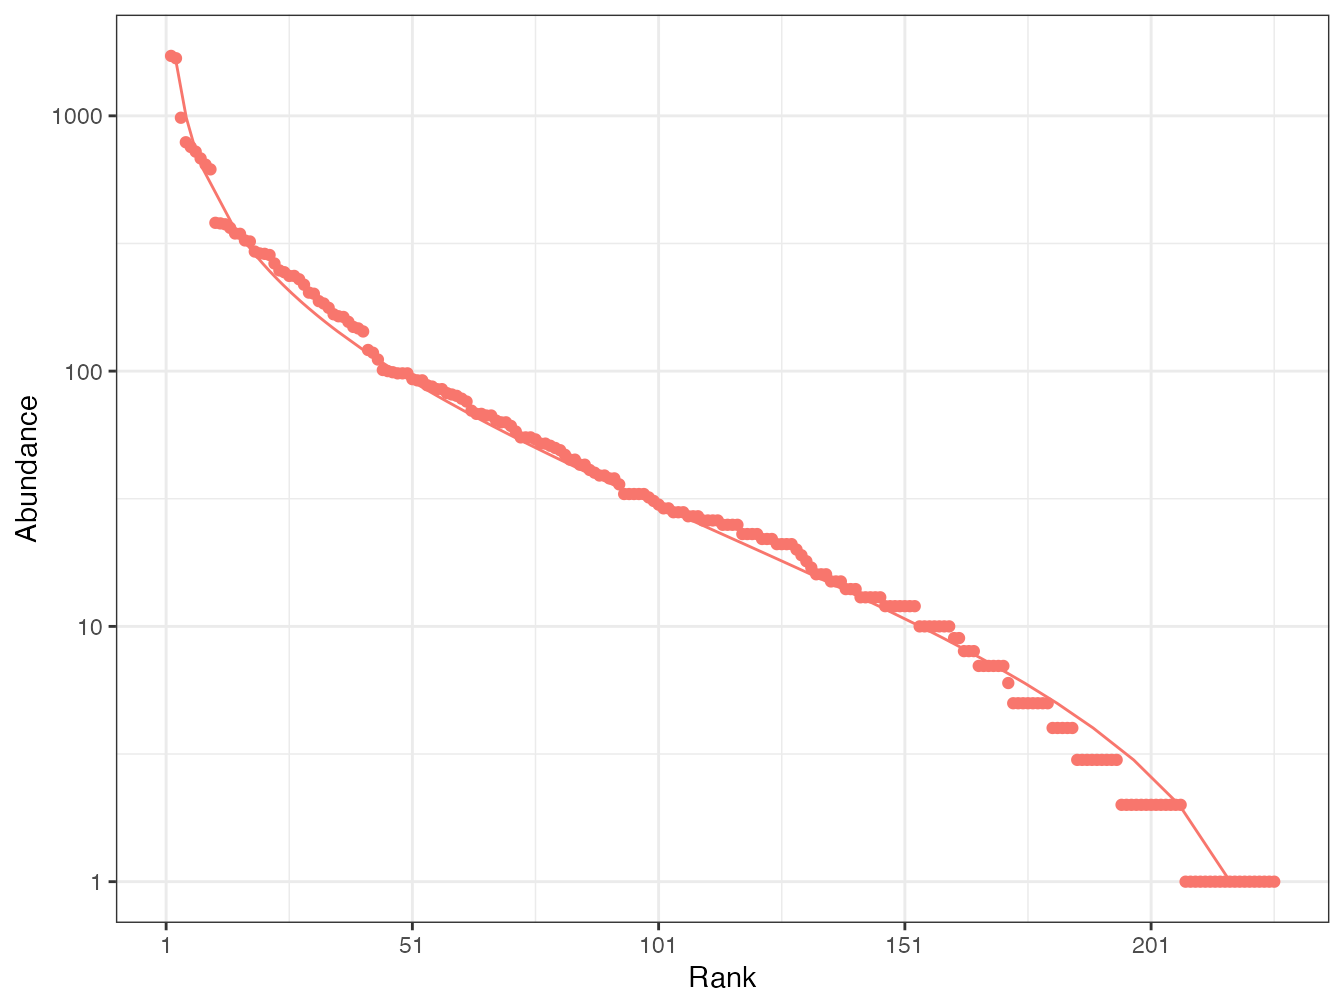
\includegraphics[width=0.8\linewidth]{MesuresBD_files/figure-latex/RACFig-1} 

}

\caption{Diagramme rang-abondance (diagramme de Whittaker) des arbres du dispositif de Barro Colorado Island. Les points sont les données: en abscisse: le rang de l'espèce, à partir de la plus abondante; en ordonnée: l'abondance de l'espèce. La courbe est l'ajustement d'une distribution log-normale.}\label{fig:RACFig}
\end{SCfigure}

\normalsize

Code de la figure \ref{fig:SADFig}:

\scriptsize

\begin{Shaded}
\begin{Highlighting}[]
\NormalTok{BCI\_abd }\OtherTok{\textless{}{-}} \FunctionTok{sort}\NormalTok{(}\FunctionTok{colSums}\NormalTok{(BCI), }\AttributeTok{decreasing =} \ConstantTok{TRUE}\NormalTok{)}
\FunctionTok{ggplot}\NormalTok{(}\FunctionTok{data.frame}\NormalTok{(BCI\_abd), }\FunctionTok{aes}\NormalTok{(BCI\_abd)) }\SpecialCharTok{+} 
  \FunctionTok{geom\_histogram}\NormalTok{(}
    \AttributeTok{bins =} \FunctionTok{nclass.Sturges}\NormalTok{(}\FunctionTok{log}\NormalTok{(BCI\_abd)), }
    \AttributeTok{color =} \StringTok{"black"}\NormalTok{, }
    \AttributeTok{fill =} \StringTok{"white"}\NormalTok{,}
    \AttributeTok{boundary =} \DecValTok{0}
\NormalTok{  ) }\SpecialCharTok{+}
  \FunctionTok{scale\_x\_log10}\NormalTok{() }\SpecialCharTok{+}
  \FunctionTok{labs}\NormalTok{(}
    \AttributeTok{x =} \StringTok{"Effectifs (échelle logarithmique)"}\NormalTok{, }
    \AttributeTok{y =} \StringTok{"Nombre d\textquotesingle{}espèces"}
\NormalTok{  )}
\end{Highlighting}
\end{Shaded}

\normalsize

Code de la figure \ref{fig:RACFig}:

\scriptsize

\begin{Shaded}
\begin{Highlighting}[]
\FunctionTok{library}\NormalTok{(}\StringTok{"divent"}\NormalTok{)}
\NormalTok{BCI\_abd }\SpecialCharTok{\%\textgreater{}\%} 
  \FunctionTok{as\_abundances}\NormalTok{() }\SpecialCharTok{\%\textgreater{}\%} 
  \FunctionTok{autoplot}\NormalTok{(}\AttributeTok{fit\_rac =} \ConstantTok{TRUE}\NormalTok{, }\AttributeTok{distribution =} \StringTok{"lnorm"}\NormalTok{)}
\end{Highlighting}
\end{Shaded}

\normalsize

Les SAD sont traitées en détail par \textcite{Magurran1988} ou \textcite{McGill2007}.
Les principales distributions, nécessaires à la compréhension de la suite sont présentées ici:

\begin{itemize}
\tightlist
\item
  La distribution en log-séries de \textcite{Fisher1943};
\item
  La distribution géométrique \autocite{Motomura1932,Whittaker1972};
\item
  La distribution log-normale \autocite{Preston1948};
\item
  Le modèle Broken Stick \autocite{MacArthur1957}.
\end{itemize}

Formellement, la distribution des probabilités des espèces, notées \(p_s\), est à établir.

\hypertarget{la-distribution-en-log-suxe9ries}{%
\section{La distribution en log-séries}\label{la-distribution-en-log-suxe9ries}}

Cette distribution est traitée en détail dans le chapitre \ref{chap-Fisher}.

Le nombre d'espèces est lié au nombre d'individus par la relation \({\mathbb E}(S^n) = \alpha \ln(1 + n / \alpha)\) où \(S^n\) indique le nombre d'espèces observées dans un échantillon de \(n\) individus.
\(\alpha\) est le paramètre qui fixe la pente de la partie linéaire de la relation, valide dès que \(n \gg \alpha\), où le nombre d'espèces \(S^n\) augmente proportionnellement au logarithme du nombre d'individus \(\ln(n)\).

La distribution a été obtenue à partir d'inventaires de communautés de papillons en Malaisie et en Angleterre.
Le modèle est tombé en désuétude faute de confirmation empirique à l'échelle de la communauté, avant d'être remis en valeur par la théorie neutre \autocite{Hubbell2001} dans lequel la distribution de la \emph{méta-communauté} est en log-séries.

\hypertarget{la-distribution-broken-stick}{%
\section{La distribution Broken Stick}\label{la-distribution-broken-stick}}

Si les espèces se partagent les ressources ou l'espace des niches, représentées par un bâton, par un processus de cassure aléatoire et simultanée (précisément, les \(S-1\) cassures du bâton sont distribuées uniformément sur sa longueur) et que leur abondance est proportionnelle à la quantité de ressources ou d'espace de niche obtenus, alors leur distribution suit le modèle Broken Stick de \textcite{MacArthur1957}.

Parmi les distributions classiques, c'est la plus équitable: la distribution uniforme des probabilités (\(p_s = 1 / S\) pour tout \(s\)) n'est jamais approchée.

Elle est peu observée empiriquement.

\hypertarget{la-distribution-log-normale}{%
\section{La distribution log-normale}\label{la-distribution-log-normale}}

Dans une distribution log-normale, le logarithme des probabilités des espèces (notées \(p_s\) pour l'espèce \(s\)) suit une loi normale.
L'écart-type \(\sigma\) de cette distribution règle l'équitabilité de la distribution.
Son espérance est obtenue à partir du nombre d'espèces et de \(\sigma\), pour que la somme des probabilités égale 1.

\textcite{May1975} explique cette distribution par le théorème de la limite centrale: la variable aléatoire valant 1 si un individu est de l'espèce \(s\) et 0 sinon est le produit de nombreuses variables de loi inconnues valant 1 en cas de succès (germination d'une graine, survie à de nombreux évènements\ldots).
Le logarithme de ce produit est une somme de variables aléatoire dont la loi est forcément normale par application du théorème de la limite centrale.

La distribution est aussi le résultat d'un algorithme de bâton brisé (\emph{broken stick}) hiérarchique \autocite{Bulmer1974}:

\begin{itemize}
\tightlist
\item
  Si les ressources (représentées par un bâton) sont partagées une première fois aléatoirement, selon une loi quelconque,
\item
  Si chaque bâton obtenu est partagé à nouveau selon le même procédé, et que l'opération est répétée un assez grand nombre de fois,
\item
  Si l'abondance de chaque espèce est proportionnelle aux ressources dont elle dispose,
\item
  Alors la distribution des espèces est log-normale.
\end{itemize}

Ce mécanisme décrit assez bien un mécanisme de partage successif des ressources, par exemple entre groupes d'espèces de plus en plus petits, correspondant à des niches écologiques de plus en plus étroites.

D'autres arguments existent dans la littérature.
Par exemple, \textcite{Engen1996} obtiennent une distribution normale à partir d'un modèle de dynamique des populations.

La distribution log-normale décrit assez bien (mais pas exactement) une communauté locale dans le cadre de la théorie neutre \autocite{Hubbell2001} comme le montre la figure \ref{fig:RACFig}.
Le nombre d'espèces rares est un peu surestimé.
La distribution exacte est donnée par \textcite{Volkov2003}.

\hypertarget{la-distribution-guxe9omuxe9trique}{%
\section{La distribution géométrique}\label{la-distribution-guxe9omuxe9trique}}

Si les espèces se partagent les ressources selon un algorithme \emph{broken stick} séquentiel (comme dans la distribution log-normale) mais de proportion fixe \(0<k<1\), alors la distribution obtenue est géométrique.
Les abondances successives sont proportionnelles à \(k, k(1-k), k(1-k)^2, \dots, k(1-k)^s, \dots, k(1-k)^S\).

Ce modèle a été établi par \textcite{Motomura1932} cité par \textcite{May1975}.
Ses propriétés ont été étudiées par \textcite{Whittaker1972}.

C'est la distribution qui traduit l'absence de relation entre la taille de l'échantillon et l'abondance des espèces \autocite{Pueyo2007}: la distribution du logarithme de ses probabilités est uniforme.
En d'autre termes, l'ordre de grandeur de l'abondance d'une espèce est uniformément distribué.

La distribution est observée dans les communautés pionnières \autocite{Bazzaz1975}, peu diverses, ou les communautés microbiennes \autocite{Haegeman2013}.

\hypertarget{synthuxe8se}{%
\section{Synthèse}\label{synthuxe8se}}



\scriptsize

\begin{SCfigure}

{\centering 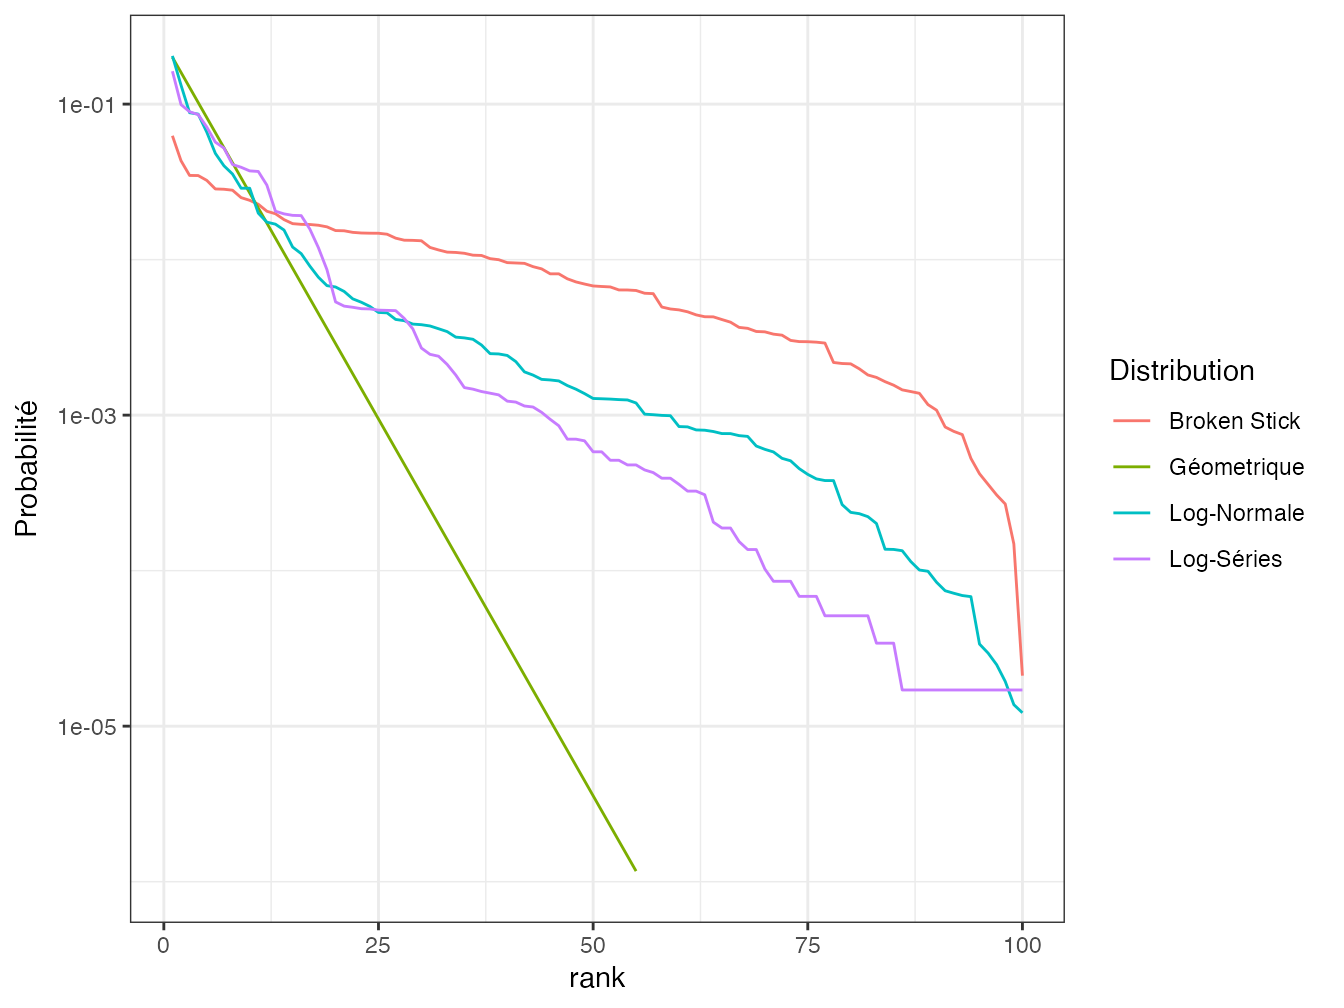
\includegraphics[width=1\linewidth]{MesuresBD_files/figure-latex/DistributionsFig-1} 

}

\caption{Diagramme rang-fréquence des distributions de probabilité classiques. Toutes les distributions sont de 100 espèces. Les probabilités inférieures à \(10^{-6}\) ne sont pas affichées. Les paramètres choisis sont \(\alpha=11\) pour la distribution log-séries, \(k=0,2\) pour la distribution géométrique et \(\sigma=2\) pour la distribution log-normale.}\label{fig:DistributionsFig}
\end{SCfigure}

\normalsize

La figure \ref{fig:DistributionsFig} est inspirée de la figure très connue de \textcite{Magurran1988}.
Elle montre bien une gradation en termes de décroissance de probabilité entre des distributions de même richesse: de la plus équitable (broken stick) à la plus inéquitable (géométrique).
Elle doit être nuancée: la proportion \(k\) de la distribution géométrique fixe la pente de la droite qui la représente sur la figure.
\(k=10\%\) sur la figure: une valeur plus faible diminuerait la pente.
De même, l'écart-type de la distribution log-normale décrit sa dispersion.
Une valeur supérieure augmenterait sa décroissance.

Le code utilisé pour produire la figure \ref{fig:DistributionsFig} est le suivant:

\scriptsize

\begin{Shaded}
\begin{Highlighting}[]
\FunctionTok{library}\NormalTok{(}\StringTok{"divent"}\NormalTok{)}
\CommentTok{\# Tirage d\textquotesingle{}une communauté en log{-}séries}
\NormalTok{size }\OtherTok{\textless{}{-}} \FloatTok{1E5}
\NormalTok{alpha }\OtherTok{\textless{}{-}} \DecValTok{11}
\NormalTok{species\_number }\OtherTok{\textless{}{-}} \SpecialCharTok{{-}}\NormalTok{alpha }\SpecialCharTok{*} \FunctionTok{log}\NormalTok{(alpha }\SpecialCharTok{/}\NormalTok{ (size }\SpecialCharTok{+}\NormalTok{ alpha))}
\NormalTok{abd\_lseries }\OtherTok{\textless{}{-}} \FunctionTok{rlseries}\NormalTok{(species\_number, size, alpha)}
\CommentTok{\# Part des ressources accaparées dans la distribution géométrique}
\NormalTok{prob }\OtherTok{\textless{}{-}} \FloatTok{0.2}
\CommentTok{\# Calcul des probabilités de la distribution géométrique}
\NormalTok{prob\_geom }\OtherTok{\textless{}{-}}\NormalTok{ prob }\SpecialCharTok{/}\NormalTok{ (}\DecValTok{1} \SpecialCharTok{{-}}\NormalTok{ (}\DecValTok{1} \SpecialCharTok{{-}}\NormalTok{ prob)}\SpecialCharTok{\^{}}\NormalTok{species\_number) }\SpecialCharTok{*}\NormalTok{ (}\DecValTok{1} \SpecialCharTok{{-}}\NormalTok{ prob)}\SpecialCharTok{\^{}}\NormalTok{(}\DecValTok{0}\SpecialCharTok{:}\NormalTok{(species\_number }\SpecialCharTok{{-}} \DecValTok{1}\NormalTok{))}
\CommentTok{\# Dispersion de la loi lognormale}
\NormalTok{sd }\OtherTok{\textless{}{-}} \DecValTok{2}
\CommentTok{\# Tirage de S valeurs dans une loi lognormale}
\NormalTok{abd\_lnorm }\OtherTok{\textless{}{-}} \FunctionTok{rlnorm}\NormalTok{(species\_number, }\AttributeTok{meanlog =} \DecValTok{0}\NormalTok{, }\AttributeTok{sdlog =}\NormalTok{ sd)}
\CommentTok{\# Tirage des probabilités de la distribution broken stick}
\NormalTok{prob\_bstick }\OtherTok{\textless{}{-}} \FunctionTok{c}\NormalTok{(cuts }\OtherTok{\textless{}{-}} \FunctionTok{sort}\NormalTok{(stats}\SpecialCharTok{::}\FunctionTok{runif}\NormalTok{(species\_number }\SpecialCharTok{{-}} \DecValTok{1}\NormalTok{)), }\DecValTok{1}\NormalTok{) }\SpecialCharTok{{-}} \FunctionTok{c}\NormalTok{(}\DecValTok{0}\NormalTok{, cuts)}
\CommentTok{\# Graphique}
\FunctionTok{tibble}\NormalTok{(}
  \AttributeTok{rank =} \DecValTok{1}\SpecialCharTok{:}\NormalTok{species\_number,}
  \StringTok{\textasciigrave{}}\AttributeTok{Log{-}Séries}\StringTok{\textasciigrave{}} \OtherTok{=} \FunctionTok{sort}\NormalTok{(abd\_lseries }\SpecialCharTok{/} \FunctionTok{sum}\NormalTok{(abd\_lseries), }\AttributeTok{decreasing =} \ConstantTok{TRUE}\NormalTok{),}
  \StringTok{\textasciigrave{}}\AttributeTok{Géometrique}\StringTok{\textasciigrave{}} \OtherTok{=} \FunctionTok{sort}\NormalTok{(prob\_geom, }\AttributeTok{decreasing =} \ConstantTok{TRUE}\NormalTok{),}
  \StringTok{\textasciigrave{}}\AttributeTok{Log{-}Normale}\StringTok{\textasciigrave{}} \OtherTok{=} \FunctionTok{sort}\NormalTok{(abd\_lnorm }\SpecialCharTok{/} \FunctionTok{sum}\NormalTok{(abd\_lnorm), }\AttributeTok{decreasing =} \ConstantTok{TRUE}\NormalTok{),}
  \StringTok{\textasciigrave{}}\AttributeTok{Broken Stick}\StringTok{\textasciigrave{}} \OtherTok{=} \FunctionTok{sort}\NormalTok{(prob\_bstick, }\AttributeTok{decreasing =} \ConstantTok{TRUE}\NormalTok{)) }\SpecialCharTok{\%\textgreater{}\%} 
  \FunctionTok{pivot\_longer}\NormalTok{(}\AttributeTok{cols =} \SpecialCharTok{{-}}\NormalTok{rank) }\SpecialCharTok{\%\textgreater{}\%} 
  \FunctionTok{ggplot}\NormalTok{() }\SpecialCharTok{+}
    \FunctionTok{geom\_line}\NormalTok{(}\FunctionTok{aes}\NormalTok{(}\AttributeTok{x =}\NormalTok{ rank, }\AttributeTok{y =}\NormalTok{ value, }\AttributeTok{color =}\NormalTok{ name)) }\SpecialCharTok{+}
    \FunctionTok{scale\_y\_log10}\NormalTok{(}\AttributeTok{limits =} \FunctionTok{c}\NormalTok{(}\FloatTok{1E{-}6}\NormalTok{, }\ConstantTok{NA}\NormalTok{)) }\SpecialCharTok{+}
    \FunctionTok{labs}\NormalTok{(}\AttributeTok{y =} \StringTok{"Probabilité"}\NormalTok{, }\AttributeTok{color =} \StringTok{"Distribution"}\NormalTok{)}
\end{Highlighting}
\end{Shaded}

\normalsize

La simulation de ces quatre distributions peut être réalisée par la fonction \texttt{rcommunity()} du package \emph{divent}, où l'argument \texttt{distribution} peut valoir \enquote{bstick}, \enquote{lnorm}, \enquote{geom} ou \enquote{lseries}.
La simulation des communautés autres que log-séries passe par le tirage des probabilités des espèces (le calcul est déterministe dans le cas de la distribution géométrique) puis le tirage d'un nombre d'individus dans une loi multinomiale respectant ces probabilités et l'effectif total.

La fonction \texttt{fit\_rac()} permet d'inférer les paramètres d'une distribution à partir d'un vecteur d'abondance.
La distribution correspondant au modèle estimé peut être affichée sur la figure Rang-Abondance (figure \ref{fig:SADFig}).

Le package \emph{sads} fournit les fonctions classiques de R (densité de probabilité, cumulative, quantile, simulation) pour les distributions utiles en écologie, au-delà de celles présentées ici.
La distribution de Volkov notamment peut être simulée.
Les fonctions \texttt{fitxxx()} complètent la fonction \texttt{fit\_rac()} de \emph{divent}.
Enfin, la fonction \texttt{radfit()} du package \emph{vegan} ajuste aux données en même temps les distributions broken-stick (désignée par \enquote{Null}), géométrique (\enquote{Preemption}) et lognormale, inclut les distributions de Zipf et de Mandelbrot non traitées ici, mais ignore les log-séries.
Les vraisemblances des différents modèles sont comparées pour choisir celui qui s'ajuste le mieux.

Le code suivant montre comment ajuster une distribution log-normale aux données de BCI avec \emph{divent} ou \emph{sads}.

\scriptsize

\begin{Shaded}
\begin{Highlighting}[]
\CommentTok{\# divent}
\FunctionTok{library}\NormalTok{(}\StringTok{"divent"}\NormalTok{)}
\NormalTok{fit\_divent\_lnorm }\OtherTok{\textless{}{-}} \FunctionTok{fit\_rac}\NormalTok{(BCI\_abd, }\AttributeTok{distribution =} \StringTok{"lnorm"}\NormalTok{)}
\CommentTok{\# Affichage des paramètres estimés}
\NormalTok{fit\_divent\_lnorm}\SpecialCharTok{$}\NormalTok{parameters}
\end{Highlighting}
\end{Shaded}

\begin{verbatim}
## # A tibble: 1 x 2
##      mu sigma
##   <dbl> <dbl>
## 1  3.14  1.79
\end{verbatim}

\begin{Shaded}
\begin{Highlighting}[]
\CommentTok{\# sads}
\FunctionTok{library}\NormalTok{(}\StringTok{"sads"}\NormalTok{)}
\CommentTok{\# Estimation. Les données sont tronquées: les espèces observées 0 fois ne sont pas comptées.}
\NormalTok{fit\_sads\_lnorm }\OtherTok{\textless{}{-}} \FunctionTok{fitlnorm}\NormalTok{(BCI\_abd, }\AttributeTok{trunc=}\DecValTok{0}\NormalTok{)}
\NormalTok{fit\_sads\_lnorm}\SpecialCharTok{@}\NormalTok{fullcoef}
\end{Highlighting}
\end{Shaded}

\begin{verbatim}
##  meanlog    sdlog 
## 3.142695 1.787195
\end{verbatim}

\begin{Shaded}
\begin{Highlighting}[]
\CommentTok{\#vegan}
\FunctionTok{library}\NormalTok{(}\StringTok{"vegan"}\NormalTok{)}
\NormalTok{fit\_vegan\_lnorm }\OtherTok{\textless{}{-}} \FunctionTok{radfit}\NormalTok{(BCI\_abd)}
\NormalTok{fit\_vegan\_lnorm}
\end{Highlighting}
\end{Shaded}

\begin{verbatim}
## 
## RAD models, family poisson 
## No. of species 225, total abundance 21457
## 
##            par1      par2     par3    Deviance AIC     
## Null                                  10261.14 11387.97
## Preemption  0.034063                   3788.38  4917.21
## Lognormal   3.3569    1.5738            744.30  1875.13
## Zipf        0.14679  -0.94912          4335.50  5466.33
## Mandelbrot  17.014   -2.0064   15.048   988.02  2120.85
##            BIC     
## Null       11387.97
## Preemption  4920.63
## Lognormal   1881.96
## Zipf        5473.16
## Mandelbrot  2131.10
\end{verbatim}

\normalsize

L'ajustement du modèle de Volkov peut être comparé à celui d'une distribution log-normale.

\scriptsize

\begin{Shaded}
\begin{Highlighting}[]
\CommentTok{\# Ajustement du modèle de Volkov}
\NormalTok{fit\_volkov }\OtherTok{\textless{}{-}} \FunctionTok{fitvolkov}\NormalTok{(BCI\_abd)}
\NormalTok{fit\_volkov}\SpecialCharTok{@}\NormalTok{fullcoef}
\end{Highlighting}
\end{Shaded}

\begin{verbatim}
##        theta            m            J 
## 4.767129e+01 9.238201e-02 2.145700e+04
\end{verbatim}

\normalsize

Graphiquement, l'ajustement est très proche mais la distribution de Volkov prévoit explicitement des effectifs égaux parce qu'entiers.

\scriptsize

\begin{Shaded}
\begin{Highlighting}[]
\CommentTok{\# Comparaison graphique des deux modèles. Log{-}normal en rouge.}
\FunctionTok{plot}\NormalTok{(}\FunctionTok{as\_abundances}\NormalTok{(BCI\_abd), }\AttributeTok{fit\_rac =} \ConstantTok{TRUE}\NormalTok{, }\AttributeTok{distribution=}\StringTok{"lnorm"}\NormalTok{)}
\CommentTok{\# Volkov en vert}
\FunctionTok{lines}\NormalTok{(}
  \FunctionTok{sort}\NormalTok{(}
    \FunctionTok{rvolkov}\NormalTok{(}
      \FunctionTok{length}\NormalTok{(BCI\_abd), }
\NormalTok{      fit\_volkov}\SpecialCharTok{@}\NormalTok{fullcoef[}\DecValTok{1}\NormalTok{], }
\NormalTok{      fit\_volkov}\SpecialCharTok{@}\NormalTok{fullcoef[}\DecValTok{2}\NormalTok{], }
\NormalTok{      fit\_volkov}\SpecialCharTok{@}\NormalTok{fullcoef[}\DecValTok{3}\NormalTok{]}
\NormalTok{    ), }
    \AttributeTok{decreasing=}\ConstantTok{TRUE}
\NormalTok{  ), }
  \AttributeTok{col=}\StringTok{"green"}
\NormalTok{)}
\end{Highlighting}
\end{Shaded}

\begin{center}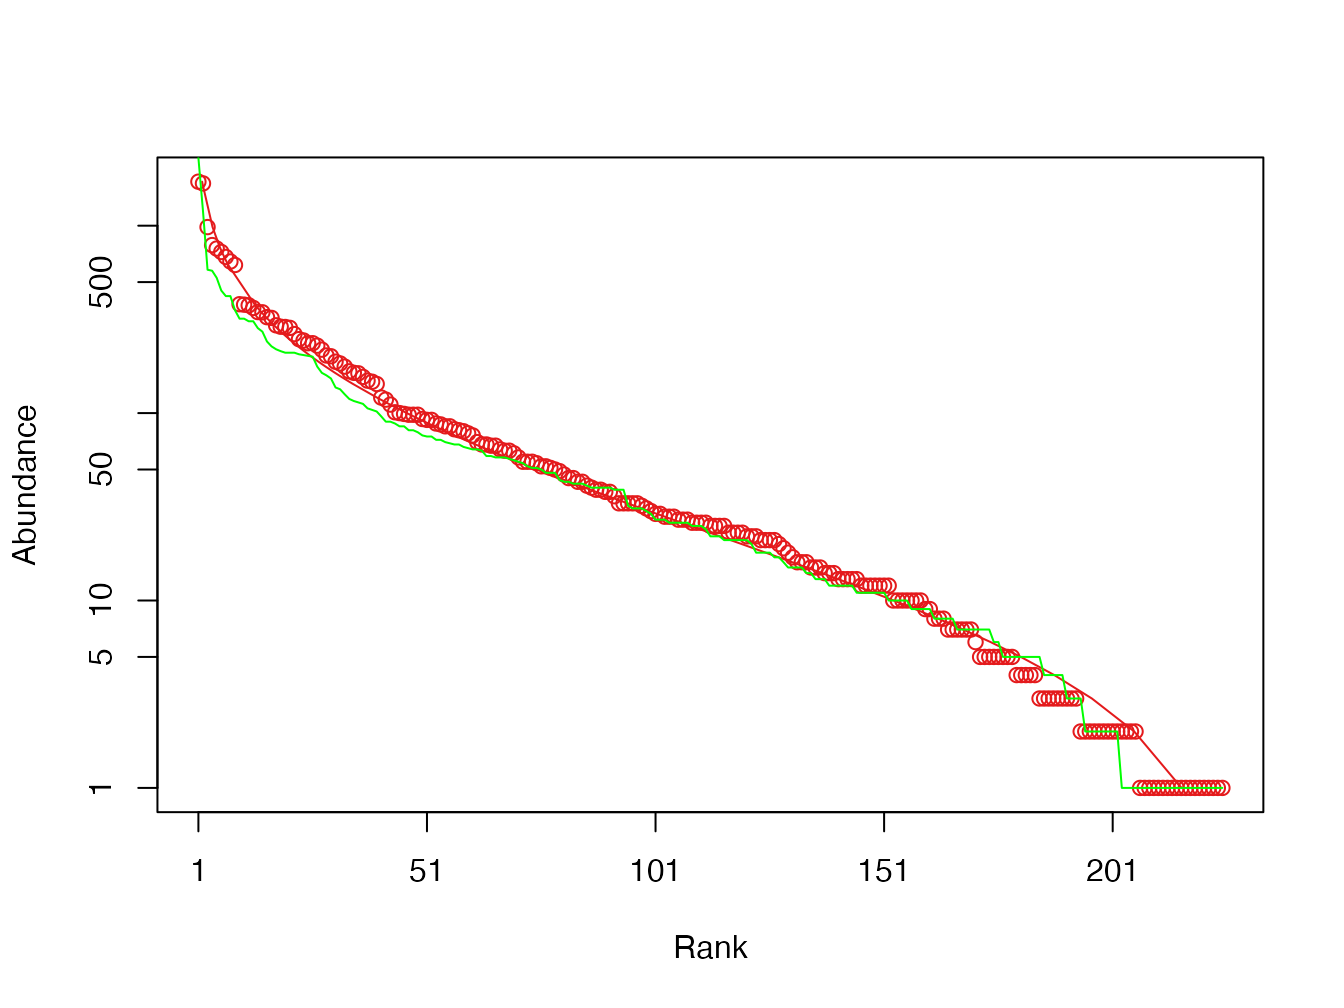
\includegraphics[width=0.8\linewidth]{MesuresBD_files/figure-latex/BCIfit3-1} \end{center}

\normalsize

Les vraisemblances sont proches.

\scriptsize

\begin{Shaded}
\begin{Highlighting}[]
\CommentTok{\# Comparaison des vraisemblances}
\NormalTok{fit\_sads\_lnorm}\SpecialCharTok{@}\NormalTok{min}
\end{Highlighting}
\end{Shaded}

\begin{verbatim}
## [1] 1157.013
\end{verbatim}

\begin{Shaded}
\begin{Highlighting}[]
\NormalTok{fit\_volkov}\SpecialCharTok{@}\NormalTok{min}
\end{Highlighting}
\end{Shaded}

\begin{verbatim}
## [1] 1150.182
\end{verbatim}

\normalsize

Les paramètres du modèle de communauté locale de la théorie neutre sont \(\theta\), le \enquote{nombre fondamental de la biodiversité} égal à deux fois le nombre d'espèces apparaissant par pas de temps dans la méta-communauté, \(m\), le taux de migration, et \(J\), la taille de la communauté locale (qui n'est pas à proprement parler un paramètre mais une statistique décrivant les données).

La différence entre les logarithmes de vraisemblance des deux modèles en faveur du modèle de Volkov, alors que le nombre de paramètres est le même.
L'ajustement est donc meilleur mais la différence est petite et la complexité du modèle et des calculs pour l'estimer ne se justifient pas en général: le modèle de Volkov est très peu utilisé en pratique.

\hypertarget{part-diversituxe9-neutre-dune-communautuxe9}{%
\part{Diversité neutre d'une communauté}\label{part-diversituxe9-neutre-dune-communautuxe9}}

\hypertarget{chap-MesuresNeutres}{%
\chapter{\texorpdfstring{Mesures classiques de la diversité \(\alpha\) ou \(\gamma\)}{Mesures classiques de la diversité \textbackslash alpha ou \textbackslash gamma}}\label{chap-MesuresNeutres}}

\begin{Summary}
Les indices classiques de diversité sont ceux de Shannon et de Simpson, et la richesse spécifique.
Ils peuvent être estimés à partir des données d'inventaire.
L'estimation de la richesse est particulièrement difficile et fait l'objet d'une abondante littérature: les estimateurs non-paramétriques (Chao et Jackknife) sont les plus utilisés.

\end{Summary}

Les mesures classiques \autocite{Peet1974} considèrent que chaque classe d'objets est différente de toutes les autres, sans que certaines soient plus ou moins semblables.
Dans ce chapitre, les classes seront des espèces.
Les mesures sont qualifiées de neutres (\emph{species-neutral}) au sens où elles ne prennent en compte aucune caractéristique propre des espèces.
La diversité neutre est souvent appelée diversité taxonomique \autocite{Devictor2010,Stegen2011}, même si le terme peut prêter à confusion avec la diversité phylogénétique, quand la phylogénie se réduit à une taxonomie \autocite{Clarke2001,Ricotta2003c}.

Ce type de mesure n'a de sens qu'à l'intérieur d'un taxocène bien défini: sommer un nombre d'espèces d'insectes à un nombre d'espèces de mammifères a peu d'intérêt.
Ces méthodes ne sont donc pas forcément les plus adaptées à la conservation: à grande échelle, des indicateurs de biodiversité \autocite{Balmford2003} peuvent être plus pertinents.
D'autre part, les communautés sont considérées comme limitées, avec un nombre d'espèces fini: la courbe d'accumulation des espèces atteint donc théoriquement une asymptote quand l'effort d'inventaire est suffisant.
Cette approche est opposée à celle, traitée dans les chapitres \ref{chap-Fisher} et suivants, qui considère que la diversité augmente indéfiniment avec la surface \autocite{Williamson2001}, que ce soit par changement d'échelle (élargir l'inventaire ajoute de nouvelles communautés) ou, plus théoriquement, parce que les communautés réelles sont considérées comme un tirage aléatoire parmi une infinités d'espèces \autocite{Fisher1943}.

Les mesures présentées ici sont les plus utilisées: richesse, indices de Shannon et de Simpson, et l'indice de Hurlbert.
Elles sont sujettes à des biais d'estimation \autocite{Mouillot1999}, notamment (mais pas seulement) à cause des espèces non échantillonnées.

Au chapitre suivant, l'entropie HCDT permettra d'unifier ces mesures et les nombres de Hill, et de leur donner un sens intuitif.

\hypertarget{sec-Richesse}{%
\section{Richesse spécifique}\label{sec-Richesse}}

La richesse est tout simplement le nombre d'espèces présentes dans le taxocène considéré.
C'est la mesure conceptuellement la plus simple mais pratiquement la plus délicate dans des systèmes très riches comme les forêts tropicales: même avec des efforts d'inventaire considérables, il n'est en général pas possible de relever toutes les espèces rares, ce qui implique de recourir à des modèles mathématiques pour en estimer le nombre.

On ne fait pas de supposition sur la forme de la SAD (voir section \ref{sec-SAD}) quand on utilise des méthodes d'estimation non paramétriques.
Les estimateurs les plus connus sont ceux de \textcite{Chao1984} et le \emph{jackknife} \autocite{Burnham1979}.

Une alternative consiste à inférer à partir des données les paramètres d'une SAD choisie, et particulièrement le nombre total d'espèces.
Cette approche est bien moins répandue parce qu'elle suppose le bon choix du modèle et est beaucoup plus intensive en calcul.
Il n'existe pas de meilleur estimateur universel \autocite{OHara2005} et il peut être efficace d'utiliser plusieurs méthodes d'estimation de façon concurrente sur les mêmes données \autocite{Basset2012}.

\hypertarget{techniques-destimation-non-paramuxe9trique}{%
\subsection{Techniques d'estimation non paramétrique}\label{techniques-destimation-non-paramuxe9trique}}

Dans le cadre d'un échantillonnage de \(n\) individus, on observe \(f_{>0}\) espèces différentes parmi les \(S\) existantes.
Chaque individu a une probabilité \(p_s\) d'appartenir à l'espèce \(s\).

On ne sait rien sur la loi des \(p_s\).
On sait seulement, comme les individus sont tirés indépendamment les uns des autres, que l'espérance du nombre \(n_s\) d'individus de l'espèce \(s\) observé dans l'échantillon est \(np_s\).
La probabilité de ne pas observer l'espèce est \((1-p_s)^n\).

Pour les espèces fréquentes, \(np_s\) est grand, et les espèces sont observées systématiquement.
La difficulté est due aux espèces pour lesquelles \(np_s\), l'espérance du nombre d'observations, est petit.
La probabilité de les observer est donnée par la loi binomiale: si \(np_s\) est proche de 0, la probabilité d'observer un individu est faible.

Les estimateurs non paramétriques cherchent à tirer le maximum d'information de la distribution des abondances \(n_s\) pour estimer le nombre d'espèces non observées.
Une présentation détaillée du problème et des limites à sa résolution est fournie par \textcite{Mao2005} qui concluent notamment que les estimateurs ne peuvent fournir qu'une borne inférieure de l'intervalle des possibles valeurs du nombre réel d'espèces.

\hypertarget{chao1-et-chao2}{%
\subsubsection{Chao1 et Chao2}\label{chao1-et-chao2}}

\textcite{Chao1984} estime le nombre d'espèces non observées à partir de celles observées 1 ou 2 fois.

Dans un échantillon de taille \(n\) résultant d'un tirage indépendant des individus, la probabilité que l'espèce \(s\) soit observée \(\nu\) fois est obtenue en écrivant la probabilité de tirer dans l'ordre \(\nu\) fois l'espèce \(s\) puis \(n-\nu\) fois une autre espèce, multiplié par le nombre de combinaisons possible pour prendre en compte l'ordre des tirages:
\begin{equation}
  \label{eq:psnu}
  p_{s, \nu}(n) = \binom{n}{\nu} {p_s^\nu \left( 1 - p_s \right)^{n - \nu}}.
\end{equation}

L'espérance du nombre d'espèces observées \(\nu\) fois, \({\mathbb E}(f_{\nu})\), est obtenue en sommant pour toutes les espèces la probabilité de les observer \(\nu\) fois:
\begin{equation}
  \label{eq:Esnnu}
  {\mathbb E}\left( f_{\nu} \right) = \binom{n}{\nu} \sum_s{p_s^\nu \left( 1 - p_s \right)^{n - \nu}}.
\end{equation}

Le carré de la norme du vecteur en \(S\) dimensions dont les coordonnées sont \((1 - p_s)^{n / 2}\) est
\[\sum_s{(1 - p_s)^n},\]
c'est-à-dire \({\mathbb E}(f_{0})\), l'espérance du nombre d'espèces non observées.
Celui du vecteur de coordonnées \(p_s (1 - p_s)^{n / 2 - 1}\) est
\[\sum_s{p_s^2 (1 - p_s)^{n - 2}} = \frac{2}{n (n - 1)}{\mathbb E}(f_{2}).\]
Enfin, le produit scalaire des deux vecteurs vaut
\[\sum_s{p_s (1 - p_s)^{n - 1}} = \frac{1}{n}{\mathbb E}(f_{1}).\]

L'inégalité de Cauchy-Schwarz (le produit scalaire est inférieur au produit des normes des vecteurs) peut être appliquée aux deux vecteurs (tous les termes sont au carré):
\begin{equation}
  \label{eq:CauchySchwarz}
  \left[ \sum_s{(1 - p_s)^n} \right] \left[ \sum_s{p_s^2 (1 - p_s)^{n-2}} \right] 
   \ge \left[ \sum_s{p_s (1 - p_s)^{n-1}} \right]^2,
\end{equation}

d'où
\begin{equation}
  \label{eq:Esn0}
  {\mathbb E}(f_{0}) 
  \ge \frac{n - 1}{n}\frac{\left[ {\mathbb E}(f_{1}) \right]^2}{2 {\mathbb E}(f_{2})}.
\end{equation}

L'estimateur est obtenu en remplaçant les espérances par les valeurs observées:

\begin{equation}
  \label{eq:Chao1}
  {\hat{S}}_\mathit{Chao1} 
   = f_{>0} + \frac{\left(n - 1 \right){\left( f_{1} \right)}^2}{2n {f_{2}}},
\end{equation}

où \(f_{>0}\) est le nombre d'espèces différentes observé.

Il s'agit d'un estimateur minimum: l'espérance du nombre d'espèces est supérieure ou égale au nombre estimé.

\textcite{Beguinot2014} a montré que l'estimateur est sans biais si le nombre d'espèces non observées décroît exponentiellement avec la taille de l'échantillon:
\begin{equation}
  \label{eq:BiaisChao}
  f_{0} = S e^{-kn},
\end{equation}
où \(k\) est un réel strictement positif.
Cette relation est cohérente avec un échantillonnage poissonien dans lequel la densité des individus est constante: voir le chapitre \ref{chap-Accumulation}.

Si aucune espèce n'est observée deux fois, l'estimateur est remplacé par
\begin{equation}
  \label{eq:Chao1sansf2}
  {\hat{S}}_\mathit{Chao1} = f_{>0} + \frac{\left( n - 1 \right){f_{1}}\left( f_{1} - 1 \right)}{2n}.
\end{equation}

Si \(n\) n'est pas trop petit, les approximations suivantes sont possibles:

\begin{equation}
  \label{eq:Chao1sansn}
  \hat{S}_\mathit{Chao1}
   = {f_{>0}} + \frac{{\left( f_{1} \right)}^2}{2f_{2}}.
\end{equation}

Si aucune espèce n'est observée deux fois, l'estimateur est remplacé \autocite{Chao2004} par

\begin{equation}
  \label{eq:Chao1sansnf2}
  {\hat{S}}_\mathit{Chao1} 
  = {f_{>0}} + {f_{1}\left( f_{1} - 1 \right)} / {2}.
\end{equation}

La variance de l'estimateur est connue, mais pas sa distribution:

\begin{equation}
  \label{eq:VarChao1}
  \operatorname{Var}{\left( {\hat{S}}_\mathit{Chao1} \right)} 
  = {f_{2}}\left[ 
      \frac{1}{2}{\left( \frac{f_{1}}{f_{2}} \right)}^2 
      + {\left( \frac{f_{1}}{f_{2}} \right)}^3 
      + \frac{1}{4}{\left( \frac{f_{1}}{f_{2}} \right)}^4
    \right].
\end{equation}

Si aucune espèce n'est observée deux fois:

\begin{equation}
  \label{eq:VarChao1sansf2}
  \operatorname{Var}{\left( {\hat{S}}_\mathit{Chao1} \right)}
  = \frac{f_{1}\left(f_{1}-1\right)}{2}
    + \frac{f_{1}{\left( 2f_{1} -1 \right)}^2}{4}
    + \frac{{\left( f_{1} \right)}^4}{4f_{>0}}.
\end{equation}

\textcite{Chao1987} donne une approximation de l'intervalle de confiance à 95\% en assumant une distribution normale:

\begin{equation}
  \label{eq:ICChao1}
  f_{>0} + \frac{{\hat{S}}_\mathit{Chao1} - {f_{>0}}}{c}
  \le S
  \le {f_{>0}} + \left( {\hat{S}}_\mathit{Chao1} - {f_{>0}} \right)c,
\end{equation}

où

\begin{equation}
  \label{eq:ICChao1c}
  c = e^{
    t^{n}_{1 - \alpha / 2} \sqrt{
      \ln\left( 1 + \frac{\operatorname{Var}\left( {\hat{S}}_\mathit{Chao1} \right)}{{\left( {\hat{S}}_\mathit{Chao1} - {f_{>0}} \right)}^2} \right)
    }
  }.
\end{equation}

\textcite[eq. 8]{Eren2012} calculent un intervalle de confiance qui est plus petit quand la valeur maximum théorique du nombre d'espèces est connue, ce qui est rarement le cas en écologie.

\textcite{Chao1987} propose un estimateur du nombre d'espèces appliqué aux données de présence-absence (un certain nombre de relevés contiennent seulement l'information de présence ou absence de chaque espèce), appelé Chao2. Il est identique à Chao1 mais \(n\) est le nombre de relevés, en général trop petit pour appliquer l'approximation de Chao1.

\textcite{Chiu2014a} améliorent l'estimateur en reprenant la démarche originale de Chao mais en utilisant un estimateur plus précis du taux de couverture, \eqref{eq:CChao} au lieu de \eqref{eq:CGood}:

\begin{equation}
  \label{eq:iChao1}
  {\hat{S}}_\mathit{iChao1} 
  = {\hat{S}}_\mathit{Chao1} 
    + \frac{f_{3}}{4f_{4}}
    \,\max\left( f_{1} - \frac{f_{2}f_{3}}{2f_{4}} ; 0 \right).
\end{equation}

\textcite{Chao2017} étendent l'applicabilité de l'estimateur Chao2 à des données dans lesquelles les espèces sont notées uniquement comme singletons ou doubletons et plus, sans distinction entre doubletons et espèces plus fréquentes.
Une relation entre le nombre de doubletons et les données disponibles est fournie; sa résolution numérique (le code R nécessaire est disponible avec l'article) permet d'estimer \(f_{2}\) et de l'injecter dans l'estimateur Chao2.

\hypertarget{lestimateur-ace}{%
\subsubsection{L'estimateur ACE}\label{lestimateur-ace}}

\textcite{Chao1992} développent l'estimateur ACE (\emph{Abundance-based coverage estimator}) à travers l'estimation du taux de couverture \(C\).
L'estimateur ACE utilise toutes les valeurs de \(f_\nu\) correspondant aux espèces rares: concrètement, la valeur limite de \(\nu\) notée \(\kappa\) est fixée arbitrairement, généralement à 10.

L'estimateur prend en compte le coefficient de variation de la distribution des fréquences (\({\hat{p}}_s\)): plus les probabilités sont hétérogènes, plus le nombre d'espèces non observées sera grand.
Finalement:

\begin{equation}
  \label{eq:ACE}
  \hat{S}_{\mathit{ACE}} 
  = f_{>\kappa} + \frac{f_{\le\kappa}}{\hat{C}_\mathit{rare}} + \frac{f_{1}}{{\hat{C}}_\mathit{rare}}{\hat{\gamma}}_\mathit{rare}.
\end{equation}

\(f_{>\kappa}\) est le nombre d'espèces dites abondantes, observées plus de \(\kappa\) fois, \(f_{\le\kappa}\) le nombre d'espèces dites rares, observées \(\kappa\) fois ou moins.
\(\hat{C}_\mathit{rare}\) est le taux de couverture ne prenant en compte que les espèces rares.

L'estimateur du coefficient de variation au carré est

\begin{equation}
  \label{eq:ACEcv}
  \hat{\gamma}^{2}_\mathit{rare} 
  = \max\left( 
    \frac{
      f_{\le\kappa} \sum^{\kappa}_{\nu=1}{\nu\left( \nu - 1 \right){f_\nu}}
    }{
      \hat{C}_\mathit{rare} \left( \sum^{\kappa}_{\nu = 1}{\nu f_{\nu}} \right) \left( \sum^{\kappa}_{\nu = 1}{\nu f_{\nu}} - 1 \right)
    } - 1 ; 0
  \right).
\end{equation}

Lorsque l'hétérogénéité est très forte, un autre estimateur est plus performant:

\begin{equation}
  \label{eq:ACEcv2}
  \tilde{\gamma}^{2}_\mathit{rare} 
  = \max\left(
    {\hat{\gamma}}^2_\mathit{rare} \left( 
      1 + \frac{
        \left( 1 - {\hat{C}}_\mathit{rare} \right) \sum^{\kappa}_{\nu = 1}{\nu\left( \nu - 1 \right){f_\nu}}
      }{
        {\hat{C}}_\mathit{rare} \left( \sum^{\kappa}_{\nu = 1}{\nu f_\nu - 1} \right)
      }
    \right) ; 0 
  \right).
\end{equation}

\textcite{Chao2010a} conseillent d'utiliser le deuxième estimateur dès que \({\hat{\gamma}}^2_\mathit{rare}\) dépasse 0,8.
L'estimateur ACE donne normalement une valeur plus grande que Chao1.
Si ce n'est pas le cas, la limite des espèces rares \(\kappa\) doit être augmentée.

\hypertarget{lestimateur-jackknife}{%
\subsubsection{L'estimateur jackknife}\label{lestimateur-jackknife}}

La méthode jackknife a pour objectif de réduire le biais d'un estimateur en considérant des jeux de données dans lesquels on a supprimé un certain nombre d'observations (ce nombre est l'\emph{ordre} de la méthode).
Burnham et Overton \autocite*{Burnham1978,Burnham1979} ont utilisé cette technique pour obtenir des estimateurs du nombre d'espèces, appelés jackknife à l'ordre \(j\), prenant en compte les valeurs de \(f_1\) à \(f_j\).
Les estimateurs du premier et du deuxième ordre sont les plus utilisés en pratique:

\begin{equation}
  \label{eq:Jack1}
  \hat{S}_\mathit{J1} = {f_{>0}} + \frac{\left( n - 1 \right) f_1}{n},
\end{equation}

\begin{equation} 
  \label{eq:Jack2}
  \hat{S}_\mathit{J2} 
  = {f_{>0}} + \frac{\left( 2n - 3 \right) f_1}{n} 
    - \frac{{\left( n - 2 \right)}^2 f_2}{n \left( n - 1 \right)}.
\end{equation}

\begin{equation} 
  \label{eq:Jack3}
  \hat{S}_\mathit{J3} 
  = {f_{>0}} + \frac{\left( 3n - 6 \right) f_1}{n} 
    - \frac{\left( 3n^2 - 15n +19 \right) f_2}{n \left( n - 1 \right)}
    + \frac{{\left( n - 3 \right)}^3 f_3}{n \left( n - 1 \right) \left( n - 2 \right)}.
\end{equation}

Augmenter l'ordre du jackknife diminue le biais mais augmente la variance de l'estimateur.

\textcite{Chao1984} a montré que les estimateurs jackknife pouvaient être retrouvés par approximation de l'indice Chao1.

La variance du jackknife d'ordre 1 est \autocite{Heltshe1983}
\begin{equation} 
  \label{eq:VarJack1}
  \operatorname{Var}{\left( \hat{S}_\mathit{J1} \right)}
  = \frac{n - 1}{n} \left( \sum_{j = 1}^{n}{j^2 f_j} - \frac{f_{>0}^2}{n} \right).
\end{equation}

L'estimateur est construit à partir de l'hypothèse selon laquelle le nombre d'espèces non observées est de la forme
\[f_0(n) = \sum_{i = 1}^{\infty}{\frac{a_i}{n^i}},\]

où la notation \(f_0(n)\) est utilisée pour expliciter sa dépendance à l'effort d'échantillonnage.

Pour cette raison, \textcite{Cormack1989} affirme qu'il n'a pas de support théorique solide.
L'espérance du nombre d'espèces non observées est (eq. \eqref{eq:Esnnu}) \(\sum_s{(1 - p_s)^n}\), qui décroît beaucoup plus rapidement que \(\sum_{i}{{a_i}/{n^i}}\): l'hypothèse est bien fausse.
En revanche, pour une gamme de \(n\) fixée (de la taille de l'inventaire à une taille suffisante pour approcher la richesse asymptotique par exemple), il est toujours possible d'écrire le nombre d'espèces non observées sous la forme d'une série de puissances négatives de \(n\), comme dans l'illustration ci-dessous.

Une communauté log-normale, similaire à BCI (300 espèces, écart-type égal à 2) est simulée et un échantillon de 1000 individus est tiré.

\scriptsize

\begin{Shaded}
\begin{Highlighting}[]
\CommentTok{\# Ecart{-}type}
\NormalTok{sdlog }\OtherTok{\textless{}{-}} \DecValTok{2}
\CommentTok{\# Nombre d\textquotesingle{}espèces}
\NormalTok{S }\OtherTok{\textless{}{-}} \DecValTok{300}
\CommentTok{\# Tirage des probabilités log{-}normales}
\NormalTok{lnorm\_abd }\OtherTok{\textless{}{-}} \FunctionTok{rlnorm}\NormalTok{(S, }\DecValTok{0}\NormalTok{, sdlog)}
\NormalTok{lnorm\_prob }\OtherTok{\textless{}{-}}\NormalTok{ lnorm\_abd }\SpecialCharTok{/} \FunctionTok{sum}\NormalTok{(lnorm\_abd)}
\CommentTok{\# Taille de l\textquotesingle{}échantillon}
\NormalTok{n }\OtherTok{\textless{}{-}} \DecValTok{1000}
\CommentTok{\# Tirage d\textquotesingle{}un échantillon}
\FunctionTok{library}\NormalTok{(}\StringTok{"divent"}\NormalTok{)}
\NormalTok{abundances }\OtherTok{\textless{}{-}} \FunctionTok{rcommunity}\NormalTok{(}\DecValTok{1}\NormalTok{, }\AttributeTok{size =}\NormalTok{ n, }\AttributeTok{prob =}\NormalTok{ lnorm\_prob)}
\end{Highlighting}
\end{Shaded}

\normalsize

L'échantillon est présenté en figure \ref{fig:BiaisJack1Fig}.

Code de la figure \ref{fig:BiaisJack1Fig}:

\scriptsize

\begin{Shaded}
\begin{Highlighting}[]
\FunctionTok{autoplot}\NormalTok{(abundances, }\AttributeTok{fit\_rac =} \ConstantTok{TRUE}\NormalTok{, }\AttributeTok{distribution=}\StringTok{"lnorm"}\NormalTok{)}
\end{Highlighting}
\end{Shaded}

\normalsize

\scriptsize

\begin{SCfigure}

{\centering 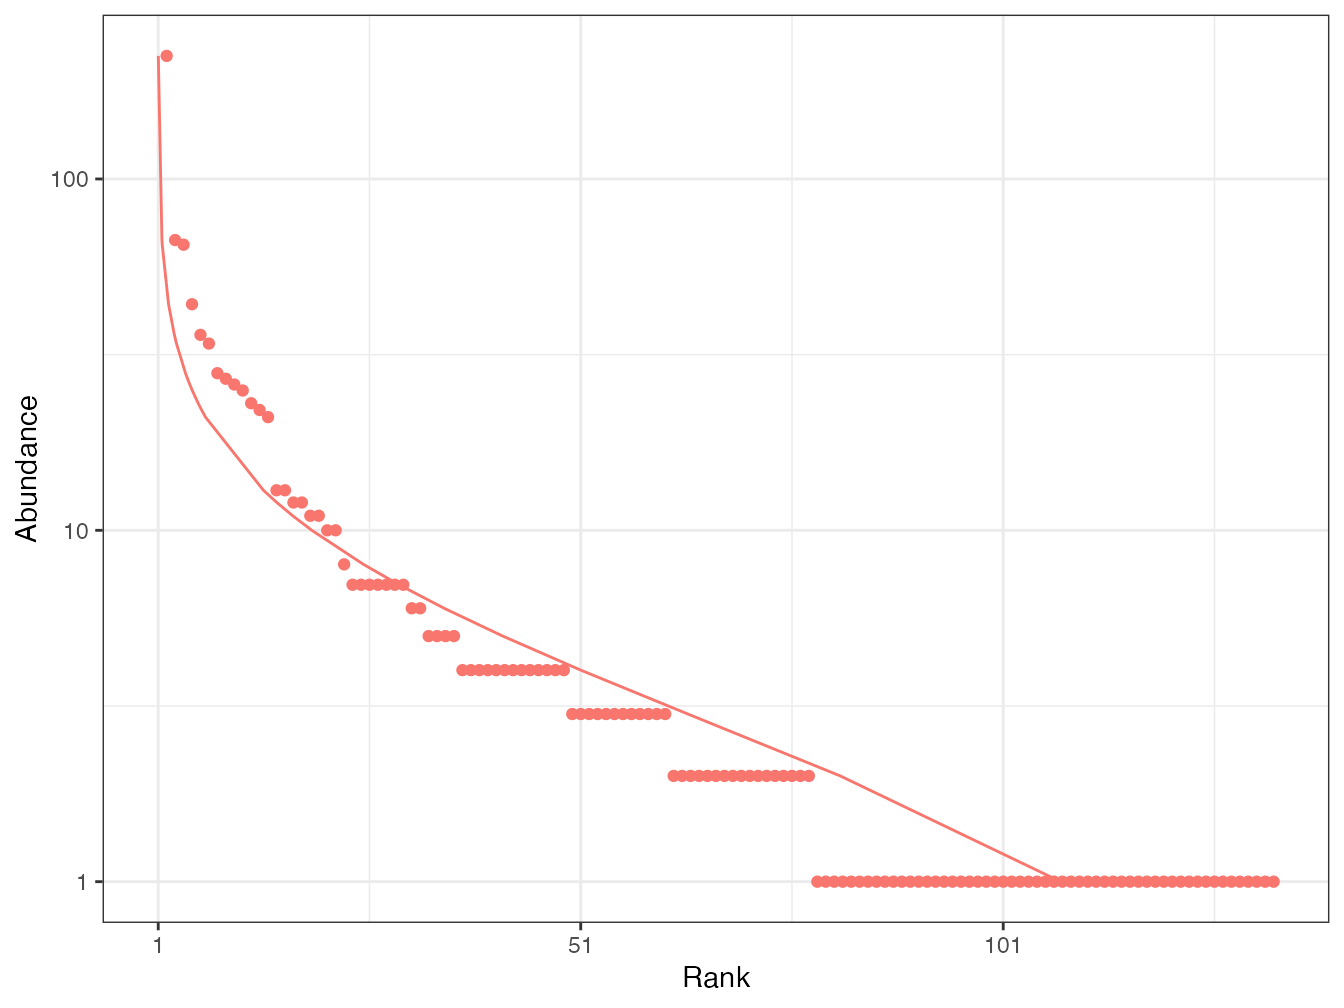
\includegraphics[width=0.8\linewidth]{MesuresBD_files/figure-latex/BiaisJack1Fig-1} 

}

\caption{Echantillon de 1000 individus tiré dans une communauté log-normale.}\label{fig:BiaisJack1Fig}
\end{SCfigure}

\normalsize

Il est possible de vérifier que l'espérance du nombre d'espèces non observées correspond bien à la moyenne des observations.

\scriptsize

\begin{Shaded}
\begin{Highlighting}[]
\CommentTok{\# Espérance des espèces non vues}
\NormalTok{E0 }\OtherTok{\textless{}{-}}\NormalTok{ (}\DecValTok{1} \SpecialCharTok{{-}}\NormalTok{ lnorm\_prob)}\SpecialCharTok{\^{}}\NormalTok{n}
\NormalTok{(f0 }\OtherTok{\textless{}{-}} \FunctionTok{sum}\NormalTok{(E0))}
\end{Highlighting}
\end{Shaded}

\begin{verbatim}
## [1] 169.7165
\end{verbatim}

\begin{Shaded}
\begin{Highlighting}[]
\CommentTok{\# Tirage de 1000 échantillons, nombre moyen d\textquotesingle{}espèces observées}
\NormalTok{(s\_obs }\OtherTok{\textless{}{-}} \FunctionTok{mean}\NormalTok{(}\FunctionTok{colSums}\NormalTok{(}\FunctionTok{rmultinom}\NormalTok{(}\DecValTok{1000}\NormalTok{, }\AttributeTok{size =}\NormalTok{ n, }\AttributeTok{prob =}\NormalTok{ lnorm\_prob) }\SpecialCharTok{\textgreater{}} \DecValTok{0}\NormalTok{)))}
\end{Highlighting}
\end{Shaded}

\begin{verbatim}
## [1] 130.37
\end{verbatim}

\begin{Shaded}
\begin{Highlighting}[]
\CommentTok{\# Vérification: nombre d\textquotesingle{}espèces observées en moyenne et non observées}
\NormalTok{s\_obs }\SpecialCharTok{+}\NormalTok{ f0}
\end{Highlighting}
\end{Shaded}

\begin{verbatim}
## [1] 300.0865
\end{verbatim}

\begin{Shaded}
\begin{Highlighting}[]
\CommentTok{\# Nombre total d\textquotesingle{}espèces dans la communauté}
\NormalTok{(S }\OtherTok{\textless{}{-}} \FunctionTok{length}\NormalTok{(lnorm\_prob))}
\end{Highlighting}
\end{Shaded}

\begin{verbatim}
## [1] 300
\end{verbatim}

\normalsize

Le nombre d'espèces non observées peut être écrit sous la forme d'une série de puissances négatives de \(n\), comme le prévoit le jackknife, entre deux valeurs de \(n\) fixées.

\scriptsize

\begin{Shaded}
\begin{Highlighting}[]
\CommentTok{\# Echantillonnage de 500 à 5000 individus}
\NormalTok{n\_seq }\OtherTok{\textless{}{-}} \DecValTok{500}\SpecialCharTok{:}\DecValTok{5000}
\CommentTok{\# Calcul du nombre d\textquotesingle{}espèces non observées}
\NormalTok{bias }\OtherTok{\textless{}{-}} \FunctionTok{sapply}\NormalTok{(n\_seq, }\ControlFlowTok{function}\NormalTok{(n) }\FunctionTok{sum}\NormalTok{((}\DecValTok{1} \SpecialCharTok{{-}}\NormalTok{ lnorm\_prob)}\SpecialCharTok{\^{}}\NormalTok{n))}
\end{Highlighting}
\end{Shaded}

\normalsize

Le nombre d'espèces non observées, qui est le biais de l'estimateur de la richesse, est présenté en figure \ref{fig:BiaisJack3Fig}.

La courbe peut être approchée par une série de puissances négatives de \(n\) dont quelques termes sont présentés sur la figure.

\scriptsize

\begin{Shaded}
\begin{Highlighting}[]
\CommentTok{\# Ordre 1}
\NormalTok{lm1 }\OtherTok{\textless{}{-}} \FunctionTok{lm}\NormalTok{(bias }\SpecialCharTok{\textasciitilde{}} \DecValTok{0} \SpecialCharTok{+} \FunctionTok{I}\NormalTok{(}\DecValTok{1}  \SpecialCharTok{/}\NormalTok{n\_seq))}
\CommentTok{\# Ordre 2}
\NormalTok{lm2 }\OtherTok{\textless{}{-}} \FunctionTok{lm}\NormalTok{(bias }\SpecialCharTok{\textasciitilde{}} \DecValTok{0} \SpecialCharTok{+} \FunctionTok{I}\NormalTok{(}\DecValTok{1} \SpecialCharTok{/}\NormalTok{ n\_seq) }\SpecialCharTok{+} \FunctionTok{I}\NormalTok{(}\DecValTok{1} \SpecialCharTok{/}\NormalTok{ n\_seq}\SpecialCharTok{\^{}}\DecValTok{2}\NormalTok{))}
\CommentTok{\# Ordre 4}
\NormalTok{lm4 }\OtherTok{\textless{}{-}} \FunctionTok{lm}\NormalTok{(}
\NormalTok{  bias }\SpecialCharTok{\textasciitilde{}} \DecValTok{0} \SpecialCharTok{+} \FunctionTok{I}\NormalTok{(}\DecValTok{1} \SpecialCharTok{/}\NormalTok{ n\_seq) }\SpecialCharTok{+} \FunctionTok{I}\NormalTok{(}\DecValTok{1} \SpecialCharTok{/}\NormalTok{ n\_seq}\SpecialCharTok{\^{}}\DecValTok{2}\NormalTok{) }\SpecialCharTok{+} \FunctionTok{I}\NormalTok{(}\DecValTok{1} \SpecialCharTok{/}\NormalTok{ n\_seq}\SpecialCharTok{\^{}}\DecValTok{3}\NormalTok{) }\SpecialCharTok{+} \FunctionTok{I}\NormalTok{(}\DecValTok{1} \SpecialCharTok{/}\NormalTok{ n\_seq}\SpecialCharTok{\^{}}\DecValTok{4}\NormalTok{)}
\NormalTok{)}
\end{Highlighting}
\end{Shaded}

\normalsize

Les termes \(a_i\) de la série de puissances négatives sont estimées par des modèles linéaires.
A l'ordre 1, le modèle \emph{lm1} fournit une approximation grossière du nombre d'espèces non observées avec un seul terme (\(f_0(n) \approx a_1 / n\)).
Le modèle s'appproche de plus en plus des données en augmentant le nombre de terme.
Le modèle \emph{lm4} contient 4 termes \(a_1\) à \(a_4\) :

\scriptsize

\begin{Shaded}
\begin{Highlighting}[]
\NormalTok{lm4}\SpecialCharTok{$}\NormalTok{coefficients}
\end{Highlighting}
\end{Shaded}

\begin{verbatim}
##    I(1/n_seq)  I(1/n_seq^2)  I(1/n_seq^3)  I(1/n_seq^4) 
##  5.663927e+05 -8.042330e+08  5.199467e+11 -1.184486e+14
\end{verbatim}

\normalsize
A partir de 6 termes, les valeurs du biais d'estimation sont presque parfaitement estimées.



\scriptsize

\begin{SCfigure}

{\centering 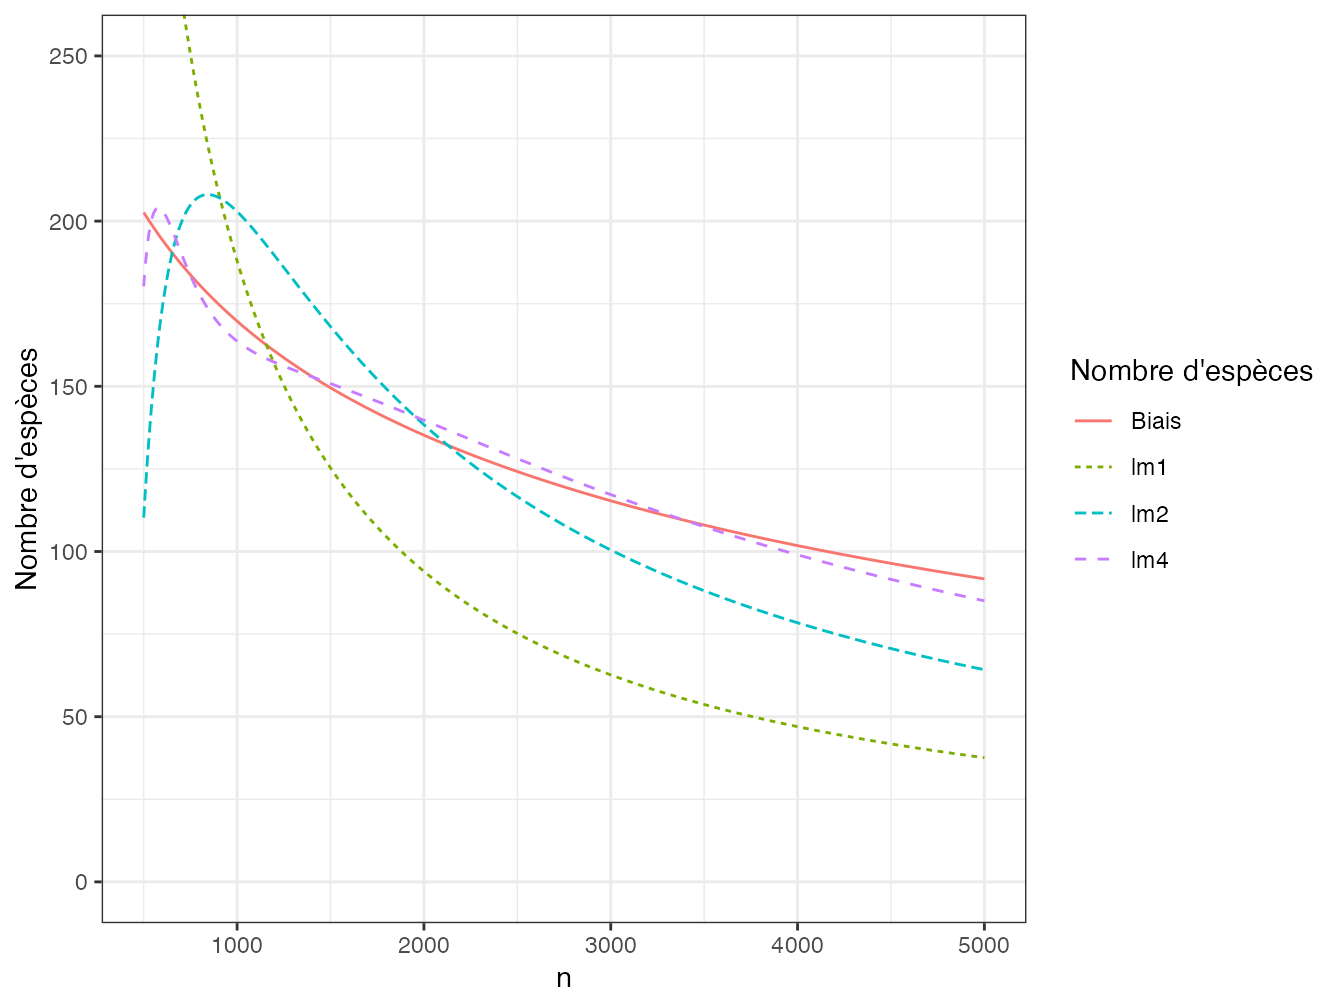
\includegraphics[width=0.8\linewidth]{MesuresBD_files/figure-latex/BiaisJack3Fig-1} 

}

\caption{Nombre d'espèces non observées dans un échantillon de taille croissante et sa décomposition en séries de puissances négatives de \(n\). Le nombre d'espèces non observées est représenté par la courbe continue. Les séries de puissances négatives d'ordre 1, 2 et 4, notées \emph{lm1} à \emph{lm4}, sont représentées en pointillés. Les courbes d'ordre 6 et plus sont confondues avec la courbe noire.}\label{fig:BiaisJack3Fig}
\end{SCfigure}

\normalsize

Code de la figure \ref{fig:BiaisJack3Fig}:

\scriptsize

\begin{Shaded}
\begin{Highlighting}[]
\FunctionTok{tibble}\NormalTok{(}
  \AttributeTok{n =}\NormalTok{ n\_seq, }
  \AttributeTok{Biais =}\NormalTok{ bias, }
  \AttributeTok{lm1 =} \FunctionTok{predict}\NormalTok{(lm1),}
  \AttributeTok{lm2 =} \FunctionTok{predict}\NormalTok{(lm2), }
  \AttributeTok{lm4 =} \FunctionTok{predict}\NormalTok{(lm4)}
\NormalTok{) }\SpecialCharTok{\%\textgreater{}\%} 
  \FunctionTok{pivot\_longer}\NormalTok{(}\AttributeTok{cols =} \SpecialCharTok{{-}}\NormalTok{n) }\SpecialCharTok{\%\textgreater{}\%} 
  \FunctionTok{ggplot}\NormalTok{() }\SpecialCharTok{+}
    \FunctionTok{geom\_line}\NormalTok{(}\FunctionTok{aes}\NormalTok{(}\AttributeTok{x =}\NormalTok{ n, }\AttributeTok{y =}\NormalTok{ value, }\AttributeTok{color =}\NormalTok{ name, }\AttributeTok{lty =}\NormalTok{ name)) }\SpecialCharTok{+}
    \FunctionTok{coord\_cartesian}\NormalTok{(}\AttributeTok{ylim =} \FunctionTok{c}\NormalTok{(}\DecValTok{0}\NormalTok{, }\DecValTok{250}\NormalTok{)) }\SpecialCharTok{+}
    \FunctionTok{labs}\NormalTok{(}
      \AttributeTok{color =} \StringTok{"Nombre d\textquotesingle{}espèces"}\NormalTok{, }
      \AttributeTok{lty =} \StringTok{"Nombre d\textquotesingle{}espèces"}\NormalTok{,}
      \AttributeTok{y =} \StringTok{"Nombre d\textquotesingle{}espèces"}
\NormalTok{    )}
\end{Highlighting}
\end{Shaded}

\normalsize

L'ajustement est possible pour des valeurs de \(n\) différentes mais les coefficients \(a_i\) sont alors différents: la forme du biais n'est valide que pour une gamme de valeurs de \(n\) fixée.

\textcite{Beguinot2016} apporte un autre argument important en faveur du jackknife.
À condition que \(n\) soit suffisamment grand, l'estimateur du nombre d'espèces non observées est une fonction linéaire du nombre d'espèces observées \(\nu\) fois: \(f_1\) pour le jackknife 1, \(2 f_1 - f_2\) pour le jackknife 2 et ainsi de suite pour les ordres suivants, contrairement à l'estimateur de Chao.
Grâce à cette propriété, l'estimateur du jackknife est additif quand plusieurs groupes d'espèces disjoints sont pris en compte: l'estimation du nombre d'espèces de papillons et de scarabées inventoriées ensemble est égale à la somme des estimations des deux groupes inventoriés séparément.
Ce n'est pas le cas pour l'estimateur de Chao.

L'estimateur du jackknife est très utilisé parce qu'il est efficace en pratique, notamment parce que son ordre peut être adapté aux données.

\hypertarget{lestimateur-du-bootstrap}{%
\subsubsection{L'estimateur du bootstrap}\label{lestimateur-du-bootstrap}}

L'estimateur du bootstrap \autocite{Smith1984} est
\begin{equation} 
  \label{eq:Smith1984}
  \hat{S}_\mathit{b} = {f_{>0}} + \sum_s{(1 - p_s)^n}.
\end{equation}

Il est peu utilisé parce que le jackknife est plus performant \autocite{Colwell1994}.

\hypertarget{calcul}{%
\subsubsection{Calcul}\label{calcul}}

Ces estimateurs peuvent être calculés de façon relativement simple à l'aide du logiciel SPADE, dans sa version pour R \autocite{Chao2016c}.
Le guide de l'utilisateur présente quelques estimateurs supplémentaires et des directives pour choisir.
Il est conseillé d'utiliser Chao1 pour une estimation minimale, et ACE pour une estimation moins biaisée de la richesse.

Les intervalles de confiance de chaque estimateur sont calculés par bootstrap: même quand la variance d'un estimateur est connue, sa loi ne l'est généralement pas, et le calcul analytique de l'intervalle de confiance n'est pas possible.

Les estimateurs et leurs intervalles de confiance peuvent également être calculés avec le package \emph{vegan} qui dispose pour cela de deux fonctions: \texttt{specpool} et \texttt{estimateR}.

\texttt{specpool} est basé sur les incidences des espèces dans un ensemble de sites d'observation et donne une estimation unique de la richesse selon les méthodes Chao2, jackknife (ordre 1 et 2) et bootstrap.
L'écart-type de l'estimateur est également fourni par la fonction, sauf pour le jackknife d'ordre 2.

\texttt{estimateR} est basé sur les abondances des espèces et retourne un estimateur de la richesse spécifique par site et non global comme \texttt{specpool}.

\hypertarget{exemple}{%
\subsubsection{Exemple}\label{exemple}}

On utilise les données de Barro Colorado Island (BCI).
La parcelle a été divisée en carrés de 1~ha.
Le tableau d'entrée est un \texttt{dataframe} contenant, pour chaque espèce d'arbres (\(\mathit{DBH}\ge\) 10~cm), ses effectifs par carré.

On charge le tableau de données:

\scriptsize

\begin{Shaded}
\begin{Highlighting}[]
\FunctionTok{library}\NormalTok{(}\StringTok{"vegan"}\NormalTok{)}
\FunctionTok{data}\NormalTok{(BCI)}
\end{Highlighting}
\end{Shaded}

\normalsize

On utilise la fonction \texttt{estimateR} pour calculer la richesse des deux premiers carrés:

\scriptsize

\begin{Shaded}
\begin{Highlighting}[]
\FunctionTok{estimateR}\NormalTok{(BCI[}\DecValTok{1}\SpecialCharTok{:}\DecValTok{2}\NormalTok{,])}
\end{Highlighting}
\end{Shaded}

\begin{verbatim}
##                   1          2
## S.obs     93.000000  84.000000
## S.chao1  117.473684 117.214286
## se.chao1  11.583785  15.918953
## S.ACE    122.848959 117.317307
## se.ACE     5.736054   5.571998
\end{verbatim}

\normalsize

Le package \emph{SPECIES} \autocite{Wang2011} permet de calculer les estimateurs jackknife d'ordre supérieur à 2 et surtout choisit l'ordre qui fournit le meilleur compromis entre biais et variance.

Comparaison des fonctions sur l'ensemble du dispositif BCI (\(f_{>0}=225\), \(f_1=19\)):

\scriptsize

\begin{Shaded}
\begin{Highlighting}[]
\FunctionTok{specpool}\NormalTok{(BCI)}
\end{Highlighting}
\end{Shaded}

\begin{verbatim}
##     Species     chao chao.se  jack1 jack1.se    jack2
## All     225 236.3732 6.54361 245.58 5.650522 247.8722
##         boot  boot.se  n
## All 235.6862 3.468888 50
\end{verbatim}

\begin{Shaded}
\begin{Highlighting}[]
\FunctionTok{library}\NormalTok{(}\StringTok{"SPECIES"}\NormalTok{)}
\CommentTok{\# Distribution du nombre d\textquotesingle{}espèces (vecteur: }
\CommentTok{\# noms = nombre d\textquotesingle{}individus}
\CommentTok{\# valeurs = nombres d\textquotesingle{}espèces ayant ce nombre d\textquotesingle{}individus)}
\NormalTok{bci\_abd }\OtherTok{\textless{}{-}} \FunctionTok{colSums}\NormalTok{(BCI)}
\CommentTok{\# Mise au format requis (matrice:}
\CommentTok{\# colonne 1 = nombre d\textquotesingle{}individus}
\CommentTok{\# colonne 2 = nombres d\textquotesingle{}espèces ayant ce nombre d\textquotesingle{}individus)}
\CommentTok{\# par la fonction abd\_freq\_count dans divent}
\FunctionTok{jackknife}\NormalTok{(}\FunctionTok{as.matrix}\NormalTok{(}\FunctionTok{abd\_freq\_count}\NormalTok{(bci\_abd)))}
\end{Highlighting}
\end{Shaded}

\begin{verbatim}
## 
## Your specified order is larger than that determined by the test, 
## Therefore the order from the test is used.
\end{verbatim}

\begin{verbatim}
## $JackknifeOrder
## [1] 1
## 
## $Nhat
## [1] 244
## 
## $SE
## [1] 6.164414
## 
## $CI
##       lb  ub
## [1,] 232 256
\end{verbatim}

\normalsize

Comparaison avec la valeur de l'équation \eqref{eq:Jack1}:

\scriptsize

\begin{Shaded}
\begin{Highlighting}[]
\CommentTok{\# Nombre d\textquotesingle{}espèces par effectif observé}
\NormalTok{bci\_abd\_freq\_count }\OtherTok{\textless{}{-}} \FunctionTok{tapply}\NormalTok{(bci\_abd, bci\_abd, length)}
\CommentTok{\# Calcul direct de Jack1}
\FunctionTok{sum}\NormalTok{(bci\_abd\_freq\_count) }\SpecialCharTok{+} 
\NormalTok{  bci\_abd\_freq\_count[}\DecValTok{1}\NormalTok{] }\SpecialCharTok{*}\NormalTok{ (}\FunctionTok{sum}\NormalTok{(bci\_abd) }\SpecialCharTok{{-}} \DecValTok{1}\NormalTok{) }\SpecialCharTok{/} \FunctionTok{sum}\NormalTok{(bci\_abd)}
\end{Highlighting}
\end{Shaded}

\begin{verbatim}
##        1 
## 243.9991
\end{verbatim}

\normalsize

La valeur du jackknife 1 fournie par \texttt{specpool} est fausse.
La fonction \texttt{jackknife} de \emph{SPECIES} donne le bon résultat, avec un intervalle de confiance calculé en supposant que la distribution est normale (\(\pm\) 1,96 écart-type au seuil de 95\%).

L'estimateur du bootstrap est calculable simplement:

\scriptsize

\begin{Shaded}
\begin{Highlighting}[]
\CommentTok{\# Effectif total}
\NormalTok{bci\_n }\OtherTok{\textless{}{-}} \FunctionTok{sum}\NormalTok{(bci\_abd)}
\CommentTok{\# Probabilités}
\NormalTok{bci\_prob }\OtherTok{\textless{}{-}}\NormalTok{ bci\_abd }\SpecialCharTok{/}\NormalTok{ bci\_n}
\CommentTok{\# Estimateur du bootstrap}
\FunctionTok{length}\NormalTok{(bci\_prob) }\SpecialCharTok{+} \FunctionTok{sum}\NormalTok{((}\DecValTok{1} \SpecialCharTok{{-}}\NormalTok{ bci\_prob)}\SpecialCharTok{\^{}}\NormalTok{bci\_n)}
\end{Highlighting}
\end{Shaded}

\begin{verbatim}
## [1] 234.3517
\end{verbatim}

\normalsize

\hypertarget{sec-ChoixEstimateur}{%
\subsubsection{Choix de l'estimateur}\label{sec-ChoixEstimateur}}

Des tests empiriques poussés ont été menés par \textcite{Brose2003} pour permettre le choix du meilleur estimateur de la richesse en fonction de la complétude de l'échantillonnage \(f_{>0}/{S}\).
Les auteurs appellent cette proportion couverture (\emph{coverage}).
Le terme \emph{completeness} a été proposé par \textcite{Beck2010} pour éviter la confusion avec le taux de couverture défini par Good (vu en section \ref{sec-Couverture}).
La complétude est inférieure à la couverture: toutes les espèces ont le même poids alors que les espèces manquantes sont plus rares et pénalisent moins le taux de couverture.



\scriptsize

\begin{SCfigure}

{\centering 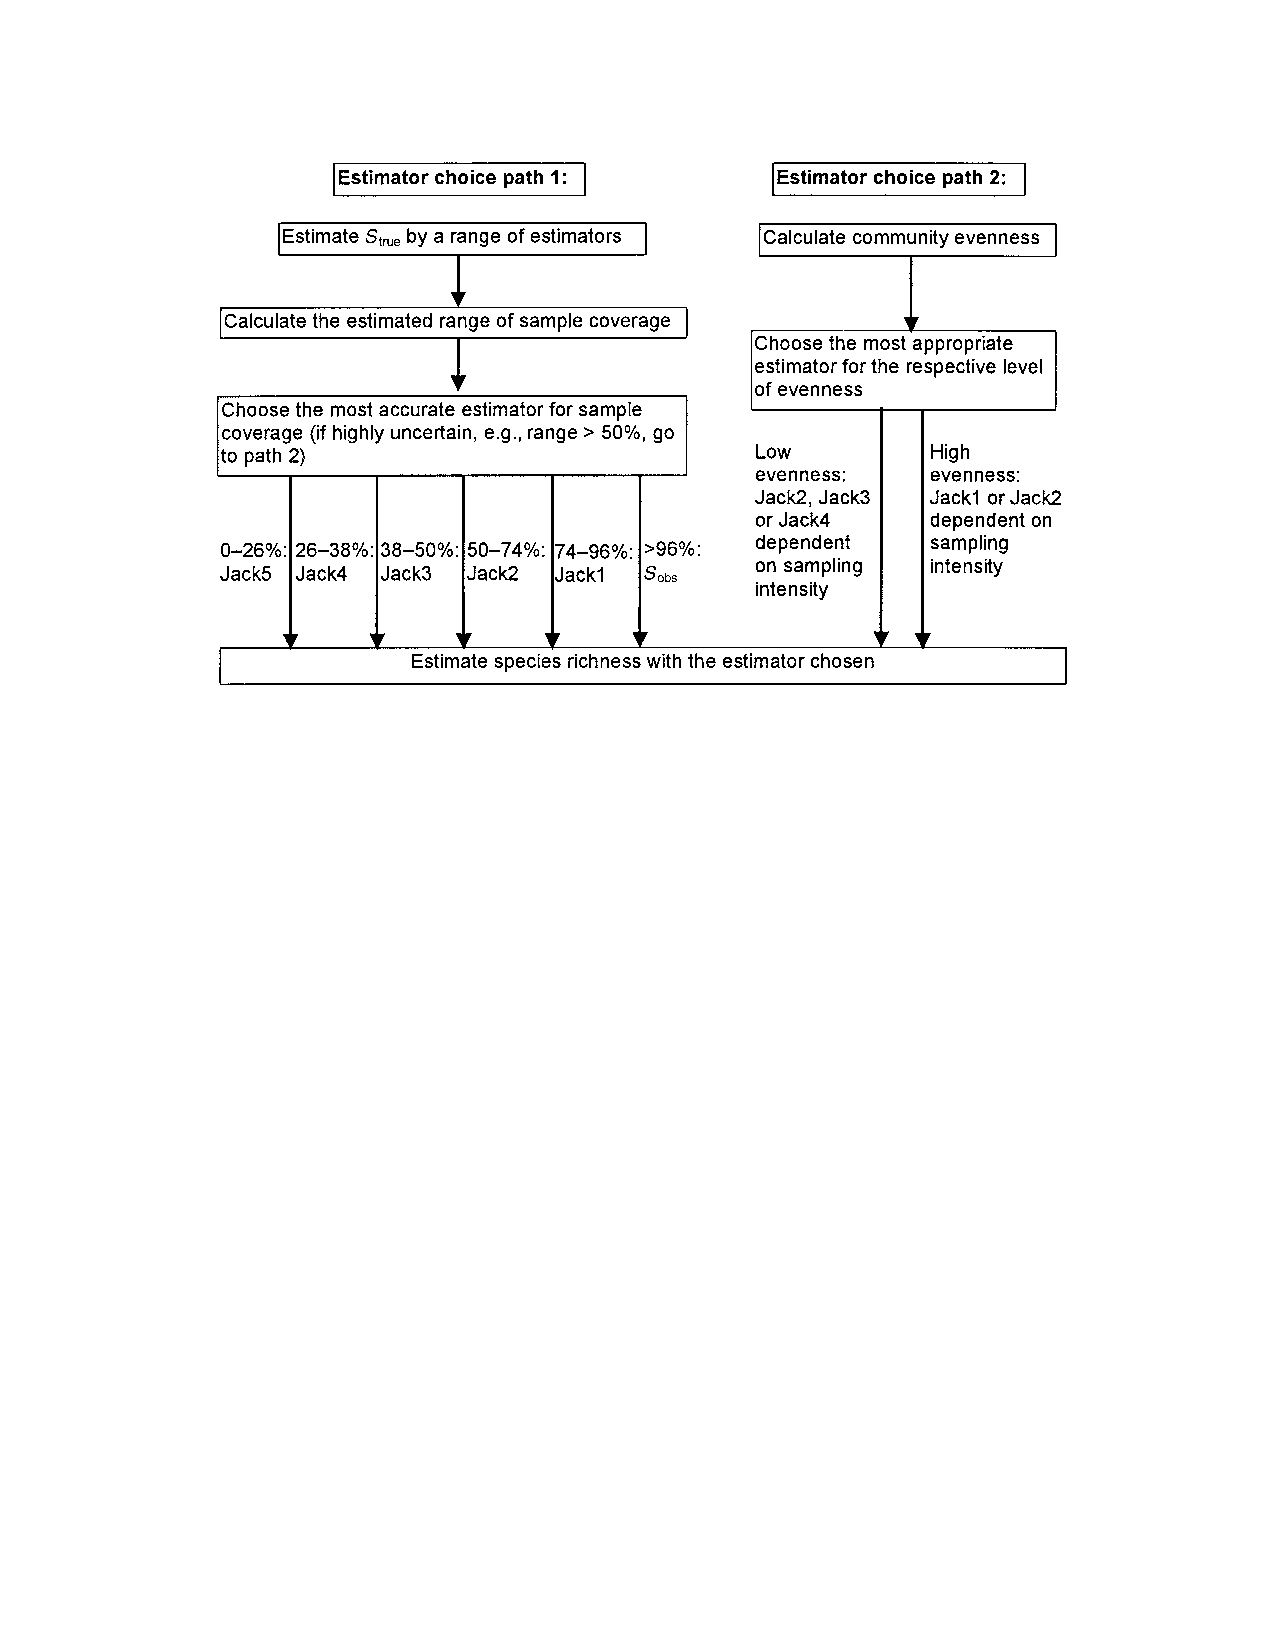
\includegraphics[width=0.8\linewidth]{images/Brose2003} 

}

\caption{Arbre de décision du meilleur estimateur du nombre d'espèces.}\label{fig:Brose2003}
\end{SCfigure}

\normalsize

Dans tous les cas, les estimateurs jackknife sont les meilleurs.
L'arbre de décision est en figure \ref{fig:Brose2003} \autocite[fig.~6]{Brose2003}.
Le choix dépend principalement de la complétude (\emph{coverage} sur la figure).
Une première estimation est nécessaire par plusieurs estimateurs.
Si les résultats sont cohérents, choisir un estimateur jackknife d'ordre d'autant plus faible que la complétude est grande.
Au-delà de 96\%, le nombre d'espèces observé est plus performant parce que les jackknifes surestiment \(S\).
S'ils sont incohérents (intervalle des estimations supérieur à 50\% de leur moyenne), le critère majeur est l'équitabilité (voir section \ref{sec-Equitabilite}).
Si elle est faible (de l'ordre de 0,5 à 0,6), les estimateurs jackknife 2 à 4 sont performants, l'ordre diminuant avec l'intensité d'échantillonnage (forte: 10\%, faible: 0,5\% de la communauté).
Pour une forte équitabilité (0,8 à 0,9), on préférera jackknife 1 ou 2.

Pour BCI, le nombre d'espèces estimé par jackknife 1 est 244.
La complétude est \({225}/{244} = 92\%\), dans le domaine de validité du jackknife 1 (74\% à 96\%) qui est donc le bon estimateur.

La parcelle 6 de Paracou nécessite l'estimateur jackknife 2:

\scriptsize

\begin{Shaded}
\begin{Highlighting}[]
\FunctionTok{library}\NormalTok{(}\StringTok{"divent"}\NormalTok{)}
\FunctionTok{div\_richness}\NormalTok{(}\FunctionTok{colSums}\NormalTok{(paracou\_6\_abd))}
\end{Highlighting}
\end{Shaded}

\begin{verbatim}
## # A tibble: 1 x 3
##   estimator   order diversity
##   <chr>       <dbl>     <dbl>
## 1 Jackknife 2     0       473
\end{verbatim}

\begin{Shaded}
\begin{Highlighting}[]
\CommentTok{\# Complétude}
\FunctionTok{div\_richness}\NormalTok{(}\FunctionTok{colSums}\NormalTok{(paracou\_6\_abd), }\AttributeTok{estimator =} \StringTok{"naive"}\NormalTok{, }\AttributeTok{as\_numeric =} \ConstantTok{TRUE}\NormalTok{) }\SpecialCharTok{/} 
  \FunctionTok{div\_richness}\NormalTok{(}\FunctionTok{colSums}\NormalTok{(paracou\_6\_abd), }\AttributeTok{as\_numeric =} \ConstantTok{TRUE}\NormalTok{)}
\end{Highlighting}
\end{Shaded}

\begin{verbatim}
## [1] 0.7082452
\end{verbatim}

\normalsize

\textcite{Chiu2014a}, à partir d'autres simulations, préfèrent l'utilisation de l'estimateur \emph{iChao1}.
Quand l'échantillonnage est suffisant, les estimateurs de Chao ont l'avantage de posséder une base théorique solide et de fournir une borne inférieure du nombre d'espèces possible.
Dans ce cas, les estimations du jackknife d'ordre 1 sont cohérentes avec celles de Chao.
En revanche, quand l'échantillonnage est insuffisant, l'estimateur jackknife d'ordre supérieur à 1 permet de réduire le biais d'estimation, au prix d'une variance accrue \autocite{Marcon2015a}.

Enfin, Beguinot \autocite*{Beguinot2015a,Beguinot2016} suggère d'utiliser en règle générale le jackknife 2 (mais ne traite pas les cas dans lesquels l'échantillonnage est trop faible pour justifier un ordre supérieur) tant que le nombre de singletons est supérieur à \(2-\sqrt(2) \approx 0,6\) fois le nombre de doubletons.
Le ratio des singletons sur les doubletons diminue quand l'échantillonnage approche de l'exhaustivité.
Quand le seuil de 0,6 est dépassé, la valeur de l'estimateur de Chao devient supérieur au jackknife 2 et doit être utilisé.
Ce seuil est cohérent avec les règles de \textcite{Brose2003}.

\hypertarget{sec-Extrapol}{%
\subsubsection{Prédiction de la richesse d'un nouvel échantillon}\label{sec-Extrapol}}

La prédiction du nombre d'espèces \(\hat{S'}\) découvert dans une nouvelle placette d'un habitat dans lequel on a déjà échantillonné est une question importante, par exemple pour évaluer le nombre d'espèces préservées dans le cadre d'une mise en réserve, ou évaluer le nombre d'espèces perdues en réduisant la surface d'une forêt.

\textcite{Shen2003} proposent un estimateur et le confrontent avec succès à des estimateurs antérieurs.
On note \(\hat{f_0}(n)\) l'estimateur du nombre d'espèces non observées dans le premier échantillon, et \(\hat{C}\) l'estimateur de son taux de couverture.
L'estimateur du nombre d'espèces du nouvel échantillon de \(n'\) individus est

\begin{equation}
  \hat{S'} 
  = \hat{f_0}(n) \left[ 
    1 - {\left( 1 - \frac{1 - \hat{C}}{\hat{f_0}(n)} \right)}^{n'} 
  \right].
\end{equation}

\(\hat{f_0}(n)\) est obtenu par la différence entre les nombres d'espèces estimé et observé: \(\hat{f_0}(n) = \hat{S} - f_{>0}(n)\).

Exemple de BCI, suite: combien de nouvelles espèces seront découvertes en échantillonnant plus?

\scriptsize

\begin{Shaded}
\begin{Highlighting}[]
\CommentTok{\# Espèces non observées}
\NormalTok{bci\_abd }\SpecialCharTok{\%\textgreater{}\%} 
  \FunctionTok{div\_richness}\NormalTok{() }\SpecialCharTok{\%\textgreater{}\%} 
  \FunctionTok{pull}\NormalTok{(diversity) }\SpecialCharTok{\%\textgreater{}\%} 
  \StringTok{\textasciigrave{}}\AttributeTok{{-}}\StringTok{\textasciigrave{}}\NormalTok{(}\FunctionTok{length}\NormalTok{(BCI\_abd)) }\SpecialCharTok{\%\textgreater{}\%} 
  \FunctionTok{print}\NormalTok{() }\OtherTok{{-}\textgreater{}}
\NormalTok{  bci\_f\_0}
\end{Highlighting}
\end{Shaded}

\begin{verbatim}
## [1] 19
\end{verbatim}

\begin{Shaded}
\begin{Highlighting}[]
\CommentTok{\# Taux de couverture}
\NormalTok{bci\_abd }\SpecialCharTok{\%\textgreater{}\%} 
\NormalTok{  coverage }\SpecialCharTok{\%\textgreater{}\%} 
  \FunctionTok{pull}\NormalTok{(coverage) }\SpecialCharTok{\%\textgreater{}\%} 
\NormalTok{  print }\OtherTok{{-}\textgreater{}} 
\NormalTok{  bci\_C}
\end{Highlighting}
\end{Shaded}

\begin{verbatim}
## [1] 0.9991146
\end{verbatim}

\normalsize



\scriptsize

\begin{SCfigure}

{\centering 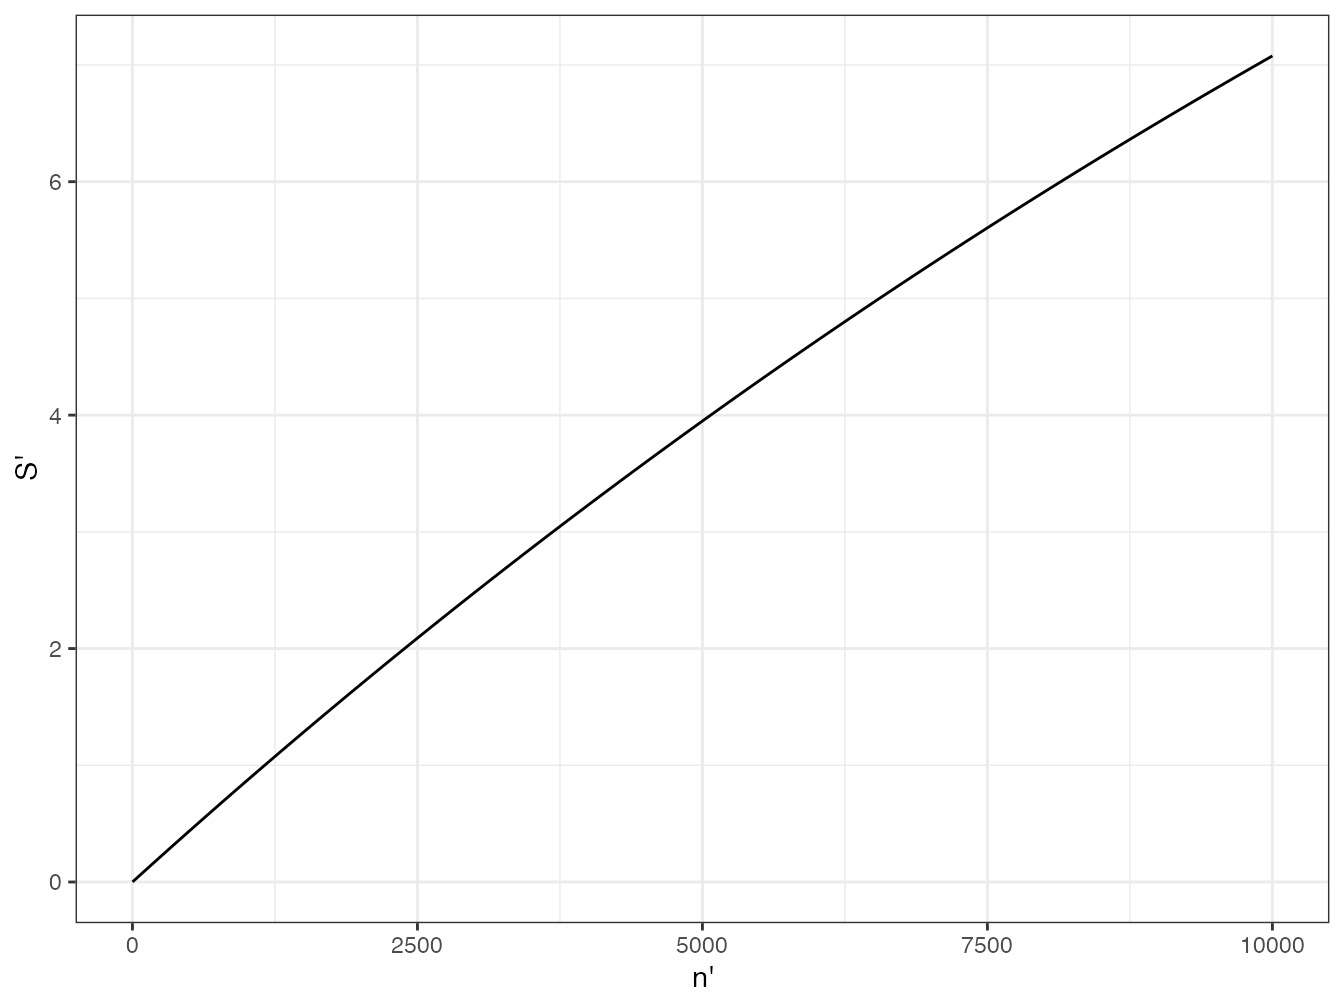
\includegraphics[width=0.8\linewidth]{MesuresBD_files/figure-latex/NonObsNFig-1} 

}

\caption{Nombre de nouvelles espèces découvertes en fonction de l'effort d'échantillonnage supplémentaire (données de BCI). Seulement 7 nouvelles espèces seront observées en échantillonnant 10000 arbres supplémentaires (environ 25 ha en plus des 50 ha de la parcelle qui contiennent 225 espèces).}\label{fig:NonObsNFig}
\end{SCfigure}

\normalsize

Le taux de couverture de l'inventaire de BCI est très proche de 100\%, donc peu de nouvelles espèces seront découvertes en augmentant l'effort d'échantillonnage.
La courbe obtenue est en figure \ref{fig:NonObsNFig}.

Le code R nécessaire pour réaliser la figure est:

\scriptsize

\begin{Shaded}
\begin{Highlighting}[]
\CommentTok{\# Nouvelles espèces en fonction du nombre de nouveaux individus}
\NormalTok{S\_prime }\OtherTok{\textless{}{-}} \ControlFlowTok{function}\NormalTok{(n\_prime, f\_0, C) \{}
\NormalTok{  f\_0 }\SpecialCharTok{*}\NormalTok{ (}\DecValTok{1} \SpecialCharTok{{-}}\NormalTok{ (}\DecValTok{1} \SpecialCharTok{{-}}\NormalTok{ (}\DecValTok{1} \SpecialCharTok{{-}}\NormalTok{ C) }\SpecialCharTok{/}\NormalTok{ f\_0)}\SpecialCharTok{\^{}}\NormalTok{n\_prime)}
\NormalTok{\}}
\CommentTok{\# Graphique}
\FunctionTok{tibble}\NormalTok{(}\AttributeTok{x =} \DecValTok{1}\SpecialCharTok{:}\DecValTok{10000}\NormalTok{) }\SpecialCharTok{\%\textgreater{}\%} 
  \FunctionTok{ggplot}\NormalTok{(}\FunctionTok{aes}\NormalTok{(x)) }\SpecialCharTok{+} 
  \FunctionTok{stat\_function}\NormalTok{(}
    \AttributeTok{fun =}\NormalTok{ S\_prime, }
    \AttributeTok{args =} \FunctionTok{list}\NormalTok{(}\AttributeTok{f\_0 =}\NormalTok{ bci\_f\_0, }\AttributeTok{C =}\NormalTok{ bci\_C)}
\NormalTok{  ) }\SpecialCharTok{+}
  \FunctionTok{labs}\NormalTok{(}\AttributeTok{x =} \StringTok{"n\textquotesingle{}"}\NormalTok{, }\AttributeTok{y =} \StringTok{"S\textquotesingle{}"}\NormalTok{)}
\end{Highlighting}
\end{Shaded}

\normalsize

La question de l'extrapolation de la richesse est traitée plus en détail dans les sections \ref{sec-RarExtrapol} et \ref{sec-Extrapolation}.

\hypertarget{infuxe9rence-du-nombre-despuxe8ces-uxe0-partir-de-la-sad}{%
\subsection{Inférence du nombre d'espèces à partir de la SAD}\label{infuxe9rence-du-nombre-despuxe8ces-uxe0-partir-de-la-sad}}

\hypertarget{distribution-de-preston}{%
\subsubsection{Distribution de Preston}\label{distribution-de-preston}}

\textcite{Preston1948} fournit dès l'introduction de son modèle log-normal une technique d'estimation du nombre total d'espèces par la célèbre méthode des octaves.
Elle est disponible dans le package \emph{vegan}:

\scriptsize

\begin{Shaded}
\begin{Highlighting}[]
\FunctionTok{veiledspec}\NormalTok{(bci\_abd)}
\end{Highlighting}
\end{Shaded}

\begin{verbatim}
## Extrapolated     Observed       Veiled 
##    235.40577    225.00000     10.40577
\end{verbatim}

\normalsize

L'ajustement direct du modèle aux données, sans regroupement par octaves \autocite{Williamson2005}, est également possible (figure \ref{fig:PrestonSansOFig}):

\scriptsize

\begin{Shaded}
\begin{Highlighting}[]
\NormalTok{bci\_preston }\OtherTok{\textless{}{-}} \FunctionTok{prestondistr}\NormalTok{(bci\_abd)}
\FunctionTok{veiledspec}\NormalTok{(bci\_preston)}
\end{Highlighting}
\end{Shaded}

\begin{verbatim}
## Extrapolated     Observed       Veiled 
##   230.931018   225.000000     5.931018
\end{verbatim}

\normalsize



\scriptsize

\begin{SCfigure}

{\centering 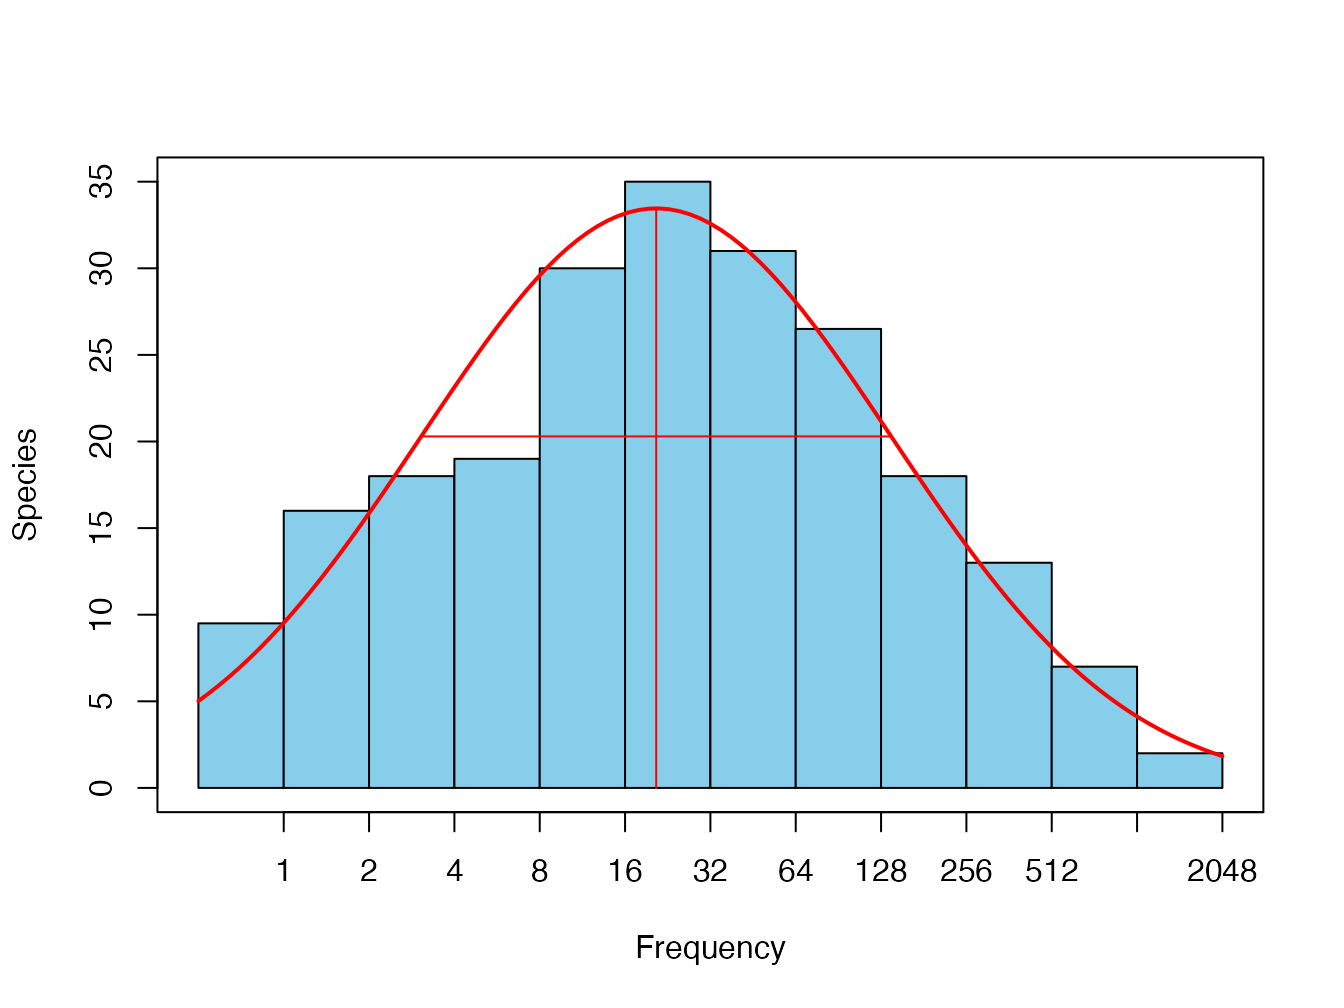
\includegraphics[width=0.8\linewidth]{MesuresBD_files/figure-latex/PrestonSansOFig-1} 

}

\caption{Ajustement du modèle de Preston aux données de BCI.}\label{fig:PrestonSansOFig}
\end{SCfigure}

\normalsize

Le code R nécessaire pour réaliser la figure est:

\scriptsize

\begin{Shaded}
\begin{Highlighting}[]
\FunctionTok{plot}\NormalTok{(bci\_preston)}
\end{Highlighting}
\end{Shaded}

\normalsize

\hypertarget{maximum-de-vraisemblance-dune-distribution-de-fisher}{%
\subsubsection{Maximum de vraisemblance d'une distribution de Fisher}\label{maximum-de-vraisemblance-dune-distribution-de-fisher}}

\textcite{Norris1998} supposent que la distribution des espèces suit le modèle de Fisher (voir chapitre \ref{chap-Fisher}) et infèrent le nombre d'espèces par maximum de vraisemblance non paramétrique (ils ne cherchent pas à inférer les paramètres de la loi de probabilité de \(p_s\) mais seulement à ajuster au mieux le modèle de Poisson aux valeurs de \({\hat{p}}_s\) observées).

Le calcul est possible avec la librairie \emph{SPECIES} de R:

\scriptsize

\begin{Shaded}
\begin{Highlighting}[]
\CommentTok{\# Mise au format requis (matrice:}
\CommentTok{\# colonne 1 = nombre d\textquotesingle{}individus}
\CommentTok{\# colonne 2 = nombres d\textquotesingle{}espèces ayant ce nombre d\textquotesingle{}individus)}
\NormalTok{bci\_abd\_freq\_count }\OtherTok{\textless{}{-}} \FunctionTok{as.matrix}\NormalTok{(}\FunctionTok{abd\_freq\_count}\NormalTok{(bci\_abd))}
\CommentTok{\# Regroupement de la queue de distribution: la longueur du vecteur est limitée à 25 pour alléger les calculs.}
\NormalTok{bci\_abd\_freq\_count[}\DecValTok{25}\NormalTok{, }\DecValTok{2}\NormalTok{] }\OtherTok{\textless{}{-}} \FunctionTok{sum}\NormalTok{(}
\NormalTok{  bci\_abd\_freq\_count[}\DecValTok{25}\SpecialCharTok{:}\FunctionTok{nrow}\NormalTok{(bci\_abd\_freq\_count), }\DecValTok{2}\NormalTok{]}
\NormalTok{)}
\NormalTok{bci\_abd\_freq\_count }\OtherTok{\textless{}{-}}\NormalTok{ bci\_abd\_freq\_count[}\DecValTok{1}\SpecialCharTok{:}\DecValTok{25}\NormalTok{, ]}
\FunctionTok{unpmle}\NormalTok{(bci\_abd\_freq\_count)}
\end{Highlighting}
\end{Shaded}

\begin{verbatim}
## Method: Unconditional NPMLE method by Norris and Pollock 1996, 1998, 
##         using algorithm by Wang and Lindsay 2005: 
## 
##         MLE=                                239 
##         Estimated Poisson mixture components:       
##         p=                                  1.10372 3.595437 10.60832 
##         pi=                                 0.402579 0.2525368 0.3448842
\end{verbatim}

\begin{verbatim}
## $Nhat
## [1] 239
\end{verbatim}

\normalsize

Le problème de cette méthode d'estimation est qu'elle diverge fréquemment.
Les calculs n'aboutissent pas si la queue de distribution n'est pas regroupée (il existe 108 valeurs différentes de \(n_s\) dans l'exemple de BCI: aucune des fonctions de \emph{SPECIES} ne fonctionne en l'état).

\textcite{Wang2005} ont amélioré sa stabilité en pénalisant le calcul de la vraisemblance:

\scriptsize

\begin{Shaded}
\begin{Highlighting}[]
\FunctionTok{pnpmle}\NormalTok{(bci\_abd\_freq\_count)}
\end{Highlighting}
\end{Shaded}

\begin{verbatim}
## Method: Penalized NPMLE method by  Wang and Lindsay 2005. 
## 
##         MLE=                                238 
##         Estimated zero-truncated Poisson mixture components:       
##         p=                                  5.784922 
##         pi=                                 1
\end{verbatim}

\begin{verbatim}
## $Nhat
## [1] 238
\end{verbatim}

\normalsize

Enfin, \textcite{Wang2010} perfectionne la technique d'estimation en supposant que les \(p_s\) suivent une loi gamma et en estimant aussi ses paramètres.
La souplesse de la loi gamma permet d'ajuster le modèle à des lois diverses et l'estimateur de Wang est très performant.

Il est disponible dans \emph{SPECIES}: fonction \texttt{pcg}.
Son défaut est qu'il nécessite un très long temps de calcul (plusieurs heures selon les données).

\scriptsize

\begin{Shaded}
\begin{Highlighting}[]
\CommentTok{\# Calcul long}
\FunctionTok{pcg}\NormalTok{(bci\_abd\_freq\_count)}
\end{Highlighting}
\end{Shaded}

\normalsize

\hypertarget{sec-RichesseSAC}{%
\subsection{Inférence du nombre d'espèces à partir de courbes d'accumulation}\label{sec-RichesseSAC}}

Cette approche consiste à extrapoler la courbe d'accumulation observée.

Le modèle le plus connu est celui de Michaelis-Menten \autocite{Michaelis1913} proposé par \textcite{Clench1979}.
En fonction de l'effort d'échantillonnage \(n\), évalué en temps (il s'agit de la collecte de papillons), le nombre d'espèces découvert augmente jusqu'à une asymptote égale au nombre d'espèces total:

\begin{equation} 
  S(n) = S\frac{n}{K + n}.
\end{equation}

\(K\) est une constante, que Clench relie à la difficulté de collecte.

L'estimation empirique du modèle de Michaelis-Menten peut être faite avec R\footnote{ Fiche TD de J.R. Lobry: \url{http://pbil.univ-lyon1.fr/R/pdf/tdr47.pdf}}.
Les 50 carrés de BCI sont utilisés pour fabriquer une courbe d'accumulation:

\scriptsize

\begin{Shaded}
\begin{Highlighting}[]
\CommentTok{\# Cumul de l\textquotesingle{}inventaire}
\CommentTok{\# Nombre d\textquotesingle{}arbres par espèce, cumulé par carré}
\NormalTok{bci\_cumul\_n\_s }\OtherTok{\textless{}{-}} \FunctionTok{apply}\NormalTok{(BCI, }\DecValTok{2}\NormalTok{, cumsum)}
\CommentTok{\# Nombre d\textquotesingle{}arbres cumulé par carré}
\NormalTok{bci\_cumul\_n }\OtherTok{\textless{}{-}} \FunctionTok{cumsum}\NormalTok{(}\FunctionTok{rowSums}\NormalTok{(BCI))}
\CommentTok{\# Nombre total d\textquotesingle{}arbres}
\NormalTok{bci\_n }\OtherTok{\textless{}{-}} \FunctionTok{sum}\NormalTok{(BCI)}
\CommentTok{\# Nombre d\textquotesingle{}espèces cumulées par carré}
\NormalTok{bci\_cumul\_S }\OtherTok{\textless{}{-}} \FunctionTok{apply}\NormalTok{(bci\_cumul\_n\_s, }\DecValTok{1}\NormalTok{, }\ControlFlowTok{function}\NormalTok{(x) }\FunctionTok{sum}\NormalTok{(x}\SpecialCharTok{\textgreater{}}\DecValTok{0}\NormalTok{))}
\end{Highlighting}
\end{Shaded}

\normalsize

Le modèle est ajusté par \texttt{nlsfit}.
Des valeurs de départ doivent être fournies pour \(K\) et \(\hat{S}\).
\(K\) est la valeur de \(n\) correspondant à \(\hat{S}^{n} = \hat{S} / 2\).
Une approximation suffisante est \(n / 4\).
Pour \(\hat{S}\), le nombre total d'espèces inventoriées est un bon choix.
Le résultat se trouve en figure \ref{fig:SobLLorFig}.

\scriptsize

\begin{Shaded}
\begin{Highlighting}[]
\CommentTok{\# Ajustement du modèle}
\NormalTok{(nlsfit }\OtherTok{\textless{}{-}} \FunctionTok{nls}\NormalTok{(}
\NormalTok{  bci\_cumul\_S }\SpecialCharTok{\textasciitilde{}}\NormalTok{ S }\SpecialCharTok{*}\NormalTok{ bci\_cumul\_n }\SpecialCharTok{/}\NormalTok{ (K }\SpecialCharTok{+}\NormalTok{ bci\_cumul\_n), }
  \AttributeTok{data =} \FunctionTok{list}\NormalTok{(bci\_cumul\_n, bci\_cumul\_S), }
  \AttributeTok{start =} \FunctionTok{list}\NormalTok{(}\AttributeTok{K =} \FunctionTok{max}\NormalTok{(bci\_cumul\_n) }\SpecialCharTok{/} \DecValTok{4}\NormalTok{, }\AttributeTok{S =} \FunctionTok{max}\NormalTok{(bci\_cumul\_S))}
\NormalTok{))}
\end{Highlighting}
\end{Shaded}

\begin{verbatim}
## Nonlinear regression model
##   model: bci_cumul_S ~ S * bci_cumul_n/(K + bci_cumul_n)
##    data: list(bci_cumul_n, bci_cumul_S)
##      K      S 
## 1251.0  232.8 
##  residual sum-of-squares: 3066
## 
## Number of iterations to convergence: 6 
## Achieved convergence tolerance: 7.861e-06
\end{verbatim}

\normalsize

L'estimation précédente utilise la méthode des moindres carrés, qui suppose l'indépendance des résidus, hypothèses évidemment violée par une courbe d'accumulation \autocite{Colwell1994}.
L'estimation par le maximum de vraisemblance est plus convenable \autocite{Raaijmakers1987}.
Elle utilise la totalité des points de la courbe d'accumulation.
La courbe d'accumulation de BCI est présentée en figure \ref{fig:specaccumFig}.
Ses données sont utilisées ici:

\scriptsize

\begin{Shaded}
\begin{Highlighting}[]
\NormalTok{bci\_sac }\OtherTok{\textless{}{-}} \FunctionTok{specaccum}\NormalTok{(BCI, }\StringTok{"random"}\NormalTok{)}
\CommentTok{\# Calculs intermédiaires}
\NormalTok{y\_i }\OtherTok{\textless{}{-}}\NormalTok{ bci\_sac}\SpecialCharTok{$}\NormalTok{richness}
\NormalTok{n }\OtherTok{\textless{}{-}} \FunctionTok{length}\NormalTok{(y\_i)}
\NormalTok{x\_i }\OtherTok{\textless{}{-}}\NormalTok{ y\_i }\SpecialCharTok{/}\NormalTok{ (}\DecValTok{1}\SpecialCharTok{:}\NormalTok{n)}
\NormalTok{x\_bar }\OtherTok{\textless{}{-}} \FunctionTok{mean}\NormalTok{(x\_i)}
\NormalTok{y\_bar }\OtherTok{\textless{}{-}} \FunctionTok{mean}\NormalTok{(y\_i)}
\NormalTok{S\_yy }\OtherTok{\textless{}{-}} \FunctionTok{sum}\NormalTok{((y\_i }\SpecialCharTok{{-}}\NormalTok{ y\_bar)}\SpecialCharTok{\^{}}\DecValTok{2}\NormalTok{)}
\NormalTok{S\_xx }\OtherTok{\textless{}{-}} \FunctionTok{sum}\NormalTok{((x\_i }\SpecialCharTok{{-}}\NormalTok{ x\_bar)}\SpecialCharTok{\^{}}\DecValTok{2}\NormalTok{)}
\NormalTok{S\_xy }\OtherTok{\textless{}{-}} \FunctionTok{sum}\NormalTok{((x\_i }\SpecialCharTok{{-}}\NormalTok{ x\_bar) }\SpecialCharTok{*}\NormalTok{ (y\_i }\SpecialCharTok{{-}}\NormalTok{ y\_bar))}
\CommentTok{\# Estimations}
\NormalTok{(K\_hat }\OtherTok{\textless{}{-}}\NormalTok{ (x\_bar }\SpecialCharTok{*}\NormalTok{ S\_yy }\SpecialCharTok{{-}}\NormalTok{ y\_bar }\SpecialCharTok{*}\NormalTok{ S\_xy) }\SpecialCharTok{/}\NormalTok{ (y\_bar }\SpecialCharTok{*}\NormalTok{ S\_xx }\SpecialCharTok{{-}}\NormalTok{ x\_bar }\SpecialCharTok{*}\NormalTok{ S\_xy))}
\end{Highlighting}
\end{Shaded}

\begin{verbatim}
## [1] 1.704586
\end{verbatim}

\begin{Shaded}
\begin{Highlighting}[]
\NormalTok{(S\_hat }\OtherTok{\textless{}{-}}\NormalTok{ y\_bar }\SpecialCharTok{+}\NormalTok{ K\_hat }\SpecialCharTok{*}\NormalTok{ x\_bar)}
\end{Highlighting}
\end{Shaded}

\begin{verbatim}
## [1] 223.5082
\end{verbatim}

\normalsize

L'estimation précédente repose sur une approximation numérique.
Le paramètre \(K\) peut être estimé plus précisément par résolution numérique de l'équation exacte du maximum de vraisemblance:

\scriptsize

\begin{Shaded}
\begin{Highlighting}[]
\CommentTok{\# Equation que K\_hat doit annuler}
\NormalTok{f }\OtherTok{\textless{}{-}} \ControlFlowTok{function}\NormalTok{(K\_hat) \{}
\NormalTok{  S\_xy }\SpecialCharTok{+} 
\NormalTok{    K\_hat }\SpecialCharTok{*}\NormalTok{ S\_xx }\SpecialCharTok{{-}} 
\NormalTok{    (S\_yy }\SpecialCharTok{+} \DecValTok{2} \SpecialCharTok{*}\NormalTok{ K\_hat }\SpecialCharTok{*}\NormalTok{ S\_xy }\SpecialCharTok{+}\NormalTok{ K\_hat}\SpecialCharTok{\^{}}\DecValTok{2} \SpecialCharTok{*}\NormalTok{ S\_xx) }\SpecialCharTok{*} \FunctionTok{sum}\NormalTok{(x\_i }\SpecialCharTok{/}\NormalTok{ (y\_i }\SpecialCharTok{+}\NormalTok{ K\_hat }\SpecialCharTok{*}\NormalTok{ x\_i) }\SpecialCharTok{/}\NormalTok{ n)}
\NormalTok{\}}
\CommentTok{\# Résolution numérique, l\textquotesingle{}intervalle de recherche doit être fourni}
\NormalTok{solution }\OtherTok{\textless{}{-}} \FunctionTok{uniroot}\NormalTok{(f, }\FunctionTok{c}\NormalTok{(}\DecValTok{0}\NormalTok{, }\FloatTok{1E+7}\NormalTok{))}
\NormalTok{(K\_hat }\OtherTok{\textless{}{-}}\NormalTok{ solution}\SpecialCharTok{$}\NormalTok{root)}
\end{Highlighting}
\end{Shaded}

\begin{verbatim}
## [1] 1.7046
\end{verbatim}

\begin{Shaded}
\begin{Highlighting}[]
\NormalTok{(S\_hat }\OtherTok{\textless{}{-}}\NormalTok{ y\_bar }\SpecialCharTok{+}\NormalTok{ K\_hat }\SpecialCharTok{*}\NormalTok{ x\_bar)}
\end{Highlighting}
\end{Shaded}

\begin{verbatim}
## [1] 223.5084
\end{verbatim}

\normalsize

Le nombre d'espèces estimé est 224, inférieur au nombre d'espèces observé.

Pour calculer l'intervalle de confiance, il est plus simple de passer par une transformation linéaire du modèle \autocite{Lineweaver1934}:

\begin{equation}
  \label{eq:Lineweaver1934}
  \left [\frac{1}{\hat{S}(n)} \right] 
  = \frac{K}{\hat{S}} \left[ \frac{1}{n} \right] + \frac{1}{\hat{S}} 
\end{equation}

Le nombre d'espèces est estimé par l'inverse de l'ordonnée à l'origine du modèle.

\scriptsize

\begin{Shaded}
\begin{Highlighting}[]
\NormalTok{y }\OtherTok{\textless{}{-}} \DecValTok{1} \SpecialCharTok{/}\NormalTok{ bci\_cumul\_S}
\NormalTok{x }\OtherTok{\textless{}{-}} \DecValTok{1} \SpecialCharTok{/}\NormalTok{ bci\_cumul\_n}
\NormalTok{lm1 }\OtherTok{\textless{}{-}} \FunctionTok{lm}\NormalTok{(y }\SpecialCharTok{\textasciitilde{}}\NormalTok{ x)}
\NormalTok{(S }\OtherTok{\textless{}{-}} \DecValTok{1}\SpecialCharTok{/}\NormalTok{lm1}\SpecialCharTok{$}\NormalTok{coef[}\DecValTok{1}\NormalTok{])}
\end{Highlighting}
\end{Shaded}

\begin{verbatim}
## (Intercept) 
##     217.002
\end{verbatim}

\normalsize



\scriptsize

\begin{SCfigure}

{\centering 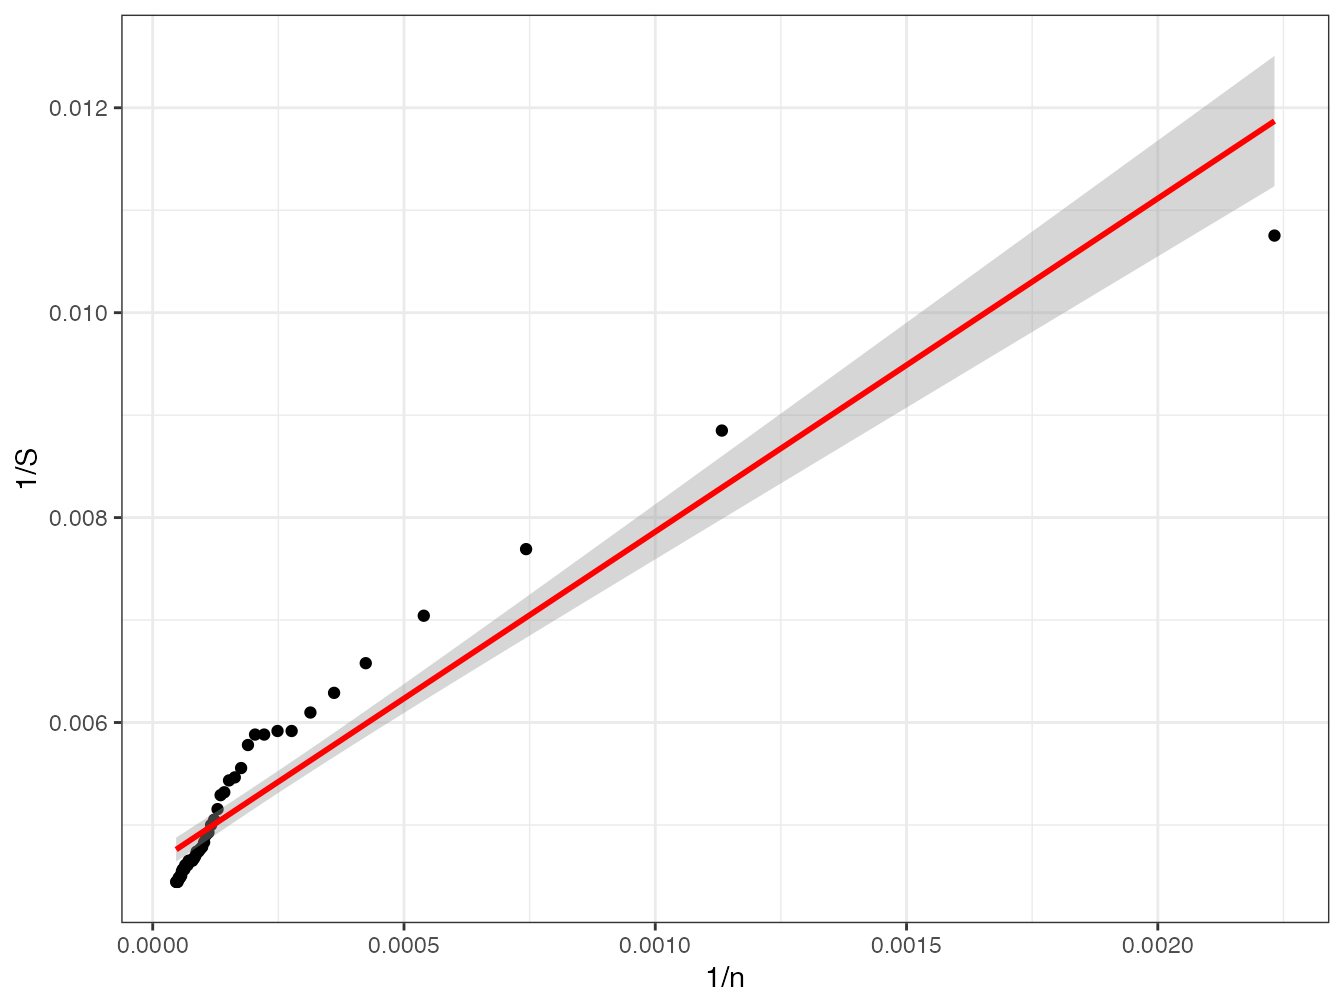
\includegraphics[width=0.8\linewidth]{MesuresBD_files/figure-latex/LineweaverFig-1} 

}

\caption{Ajustement du même modèle de Michaelis-Menten transformé selon Lineweaver et Burk.}\label{fig:LineweaverFig}
\end{SCfigure}

\normalsize

On voit assez clairement que le modèle (figure \ref{fig:LineweaverFig}) s'ajuste mal quand il est représenté sous cette forme \autocite{Raaijmakers1987}.

Le code R nécessaire pour réaliser la figure est:

\scriptsize

\begin{Shaded}
\begin{Highlighting}[]
\FunctionTok{tibble}\NormalTok{(x, y) }\SpecialCharTok{\%\textgreater{}\%} 
  \FunctionTok{ggplot}\NormalTok{(}\FunctionTok{aes}\NormalTok{(x, y)) }\SpecialCharTok{+} 
    \FunctionTok{geom\_point}\NormalTok{() }\SpecialCharTok{+}
    \FunctionTok{stat\_smooth}\NormalTok{(}\AttributeTok{method =} \StringTok{"lm"}\NormalTok{, }\AttributeTok{col =} \StringTok{"red"}\NormalTok{) }\SpecialCharTok{+}
    \FunctionTok{labs}\NormalTok{(}\AttributeTok{x =} \StringTok{"1/n"}\NormalTok{, }\AttributeTok{y=}\StringTok{"1/S"}\NormalTok{)}
\end{Highlighting}
\end{Shaded}

\normalsize

Le nombre d'espèces estimé est inférieur au nombre observé, qui ne se trouve même pas dans l'intervalle de confiance à 95\%.
Le modèle de Michaelis-Menten ne convient pas.

\textcite{Soberon1993} développent un cadre théorique plus vaste qui permet d'ajuster la courbe d'accumulation à plusieurs modèles.
Ces modèles sont efficaces empiriquement mais manquent de support théorique pour justifier leur forme.
Le modèle le plus simple est exponentiel négatif.
Si la probabilité de trouver une nouvelle espèce est proportionnelle au nombre d'espèces non encore découvertes, la courbe d'accumulation suit la relation

\begin{equation} 
  \label{eq:Soberon1993a}
  S() = S \left( 1 - e^{kn} \right).
\end{equation}

Les paramètres peuvent être estimés par la méthode des moindres carrés:

\scriptsize

\begin{Shaded}
\begin{Highlighting}[]
\NormalTok{(nlsexp }\OtherTok{\textless{}{-}} \FunctionTok{nls}\NormalTok{(}
\NormalTok{  bci\_cumul\_S }\SpecialCharTok{\textasciitilde{}}\NormalTok{ S }\SpecialCharTok{*}\NormalTok{ (}\DecValTok{1} \SpecialCharTok{{-}} \FunctionTok{exp}\NormalTok{(k }\SpecialCharTok{*}\NormalTok{ bci\_cumul\_n)), }
  \AttributeTok{data =} \FunctionTok{list}\NormalTok{(bci\_cumul\_n, bci\_cumul\_S), }
  \AttributeTok{start =} \FunctionTok{list}\NormalTok{(}\AttributeTok{S =} \FunctionTok{max}\NormalTok{(bci\_cumul\_S), }\AttributeTok{k =} \SpecialCharTok{{-}}\DecValTok{1} \SpecialCharTok{/} \DecValTok{1000}\NormalTok{)}
\NormalTok{))}
\end{Highlighting}
\end{Shaded}

\begin{verbatim}
## Nonlinear regression model
##   model: bci_cumul_S ~ S * (1 - exp(k * bci_cumul_n))
##    data: list(bci_cumul_n, bci_cumul_S)
##          S          k 
## 212.198081  -0.000494 
##  residual sum-of-squares: 10664
## 
## Number of iterations to convergence: 13 
## Achieved convergence tolerance: 8.047e-06
\end{verbatim}

\normalsize

Ce modèle, proposé par \textcite{Holdridge1971}, sous-estime la richesse parce que la probabilité de découvrir une nouvelle espèce diminue plus vite que le nombre d'espèces restant à découvrir: les dernières espèces sont plus rares et donc plus difficiles à détecter.

Un modèle plus réaliste définit cette probabilité comme une fonction décroissante du nombre d'espèces manquantes.
La fonction la plus simple est une exponentielle négative mais elle ne s'annule jamais et le nombre d'espèces n'a pas d'asymptote.
Un paramètre supplémentaire pour obtenir l'asymptote est nécessaire et aboutir à la relation

\begin{equation} 
  \label{eq:Soberon1993b}
  f = \frac{1}{z} \ln \left[ \frac{a}{c} - \frac{a-c}{c} e^{-czn} \right].
\end{equation}

Les paramètres à estimer sont \(z\), \(a\) et \(c\).

\scriptsize

\begin{Shaded}
\begin{Highlighting}[]
\NormalTok{(nlslog }\OtherTok{\textless{}{-}} \FunctionTok{nls}\NormalTok{(}
\NormalTok{  bci\_cumul\_S }\SpecialCharTok{\textasciitilde{}} \DecValTok{1} \SpecialCharTok{/}\NormalTok{ z }\SpecialCharTok{*} \FunctionTok{log}\NormalTok{(a }\SpecialCharTok{/}\NormalTok{ c }\SpecialCharTok{{-}}\NormalTok{ (a }\SpecialCharTok{{-}}\NormalTok{ c) }\SpecialCharTok{/}\NormalTok{ c }\SpecialCharTok{*} \FunctionTok{exp}\NormalTok{(}\SpecialCharTok{{-}}\NormalTok{c }\SpecialCharTok{*}\NormalTok{ z }\SpecialCharTok{*}\NormalTok{ bci\_cumul\_n)), }
  \AttributeTok{data =} \FunctionTok{list}\NormalTok{(bci\_cumul\_n, bci\_cumul\_S), }
  \AttributeTok{start =} \FunctionTok{list}\NormalTok{(}\AttributeTok{z =}\NormalTok{ .}\DecValTok{05}\NormalTok{, }\AttributeTok{a =} \DecValTok{1}\NormalTok{, }\AttributeTok{c =}\NormalTok{ .}\DecValTok{001}\NormalTok{)}
\NormalTok{))}
\end{Highlighting}
\end{Shaded}

\begin{verbatim}
## Nonlinear regression model
##   model: bci_cumul_S ~ 1/z * log(a/c - (a - c)/c * exp(-c * z * bci_cumul_n))
##    data: list(bci_cumul_n, bci_cumul_S)
##        z        a        c 
## 0.025139 0.755365 0.001114 
##  residual sum-of-squares: 446.1
## 
## Number of iterations to convergence: 4 
## Achieved convergence tolerance: 4.366e-06
\end{verbatim}

\begin{Shaded}
\begin{Highlighting}[]
\CommentTok{\# Nombre d\textquotesingle{}espèces}
\NormalTok{coefs }\OtherTok{\textless{}{-}} \FunctionTok{coef}\NormalTok{(nlslog)}
\FunctionTok{log}\NormalTok{(coefs[}\StringTok{"a"}\NormalTok{] }\SpecialCharTok{/}\NormalTok{ coefs[}\StringTok{"c"}\NormalTok{]) }\SpecialCharTok{/}\NormalTok{ coefs[}\StringTok{"z"}\NormalTok{]}
\end{Highlighting}
\end{Shaded}

\begin{verbatim}
##        a 
## 259.3128
\end{verbatim}

\normalsize



\scriptsize

\begin{SCfigure}

{\centering 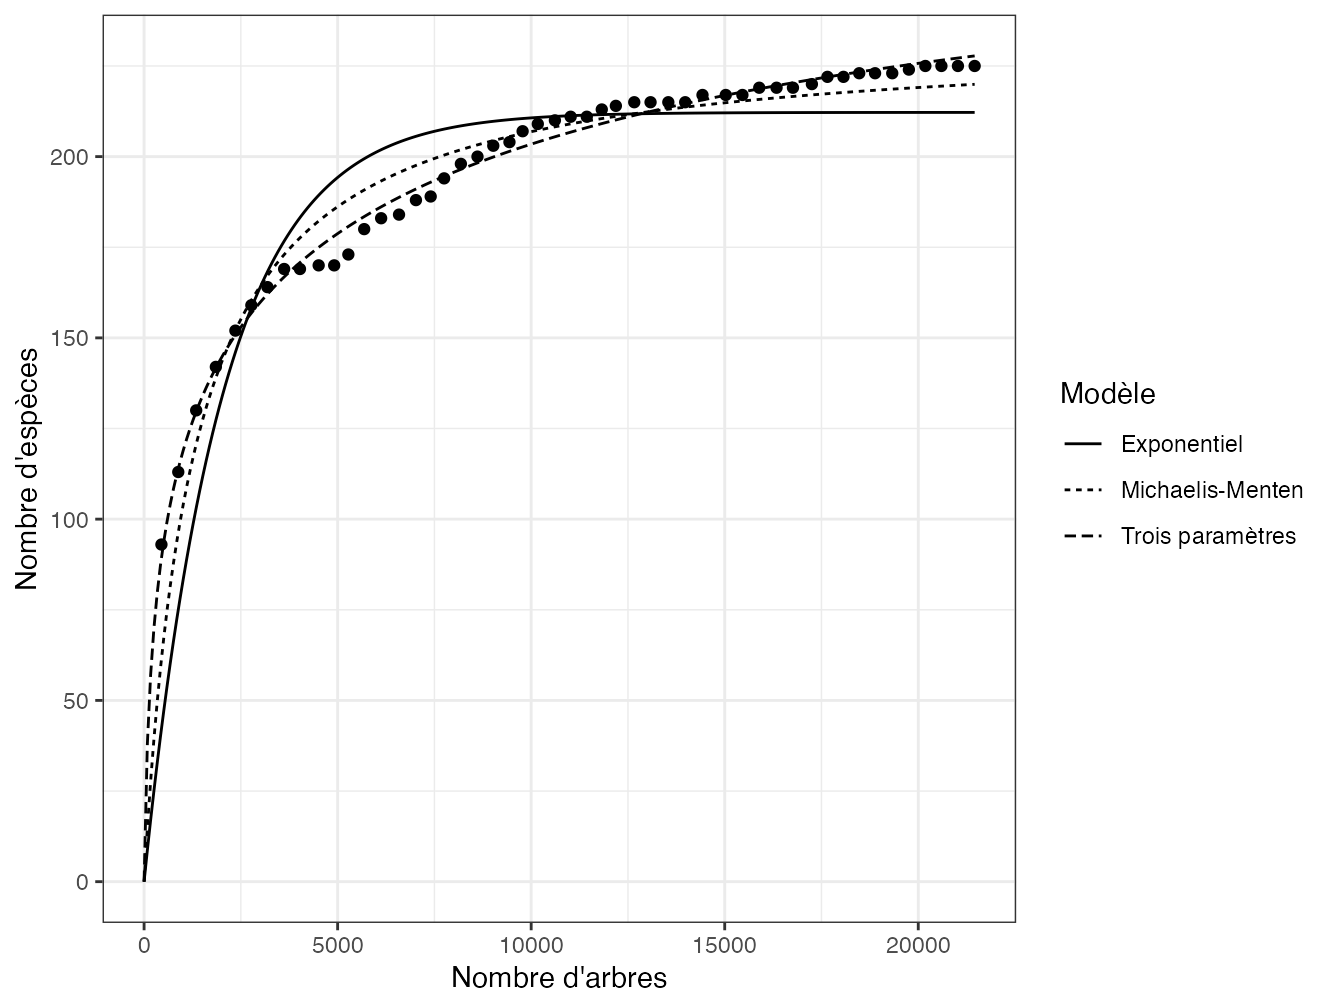
\includegraphics[width=0.8\linewidth]{MesuresBD_files/figure-latex/SobLLorFig-1} 

}

\caption{Ajustement des modèles de Michaelis-Menten et de de Soberón et Llorente (modèle exponentiel négatif et modèle à trois paramètres) aux données de BCI. Les points représentent le nombre d'espèces cumulées en fonction du nombre d'arbres. Le modèle exponentiel négatif (Holdridge) sous-estime la richesse, plus que celui de Michaelis-Menten (Clench). Le modèle à trois paramètres s'ajuste mieux aux données, mais il surestime probablement la richesse.}\label{fig:SobLLorFig}
\end{SCfigure}

\normalsize

L'estimation est cette fois supérieure à celle du jackknife (244 espèces).

La figure \ref{fig:SobLLorFig} présente les deux ajustements de modèle de Soberón et Llorente avec celui de Clench.
L'estimation de la richesse par extrapolation est plus incertaine que par les méthodes non paramétriques.
Elle est très peu utilisée.

Le code R nécessaire pour réaliser la figure est:

\scriptsize

\begin{Shaded}
\begin{Highlighting}[]
\NormalTok{x }\OtherTok{\textless{}{-}} \FunctionTok{seq}\NormalTok{(}\AttributeTok{from =} \DecValTok{0}\NormalTok{, }\AttributeTok{to =} \FunctionTok{max}\NormalTok{(bci\_cumul\_n), }\AttributeTok{length =} \DecValTok{255}\NormalTok{)}
\NormalTok{x\_new }\OtherTok{\textless{}{-}} \FunctionTok{list}\NormalTok{(}\AttributeTok{bci\_cumul\_n =}\NormalTok{ x)}
\FunctionTok{tibble}\NormalTok{(}
\NormalTok{  x, }
  \StringTok{\textasciigrave{}}\AttributeTok{Michaelis{-}Menten}\StringTok{\textasciigrave{}} \OtherTok{=} \FunctionTok{predict}\NormalTok{(nlsfit, }\AttributeTok{newdata =}\NormalTok{ x\_new),}
  \StringTok{\textasciigrave{}}\AttributeTok{Exponentiel}\StringTok{\textasciigrave{}} \OtherTok{=} \FunctionTok{predict}\NormalTok{(nlsexp, }\AttributeTok{newdata =}\NormalTok{ x\_new),}
  \StringTok{\textasciigrave{}}\AttributeTok{Trois paramètres}\StringTok{\textasciigrave{}} \OtherTok{=} \FunctionTok{predict}\NormalTok{(nlslog, }\AttributeTok{newdata =}\NormalTok{ x\_new)}
\NormalTok{) }\SpecialCharTok{\%\textgreater{}\%} 
  \FunctionTok{pivot\_longer}\NormalTok{(}\AttributeTok{cols =} \SpecialCharTok{{-}}\NormalTok{x) }\SpecialCharTok{\%\textgreater{}\%} 
  \FunctionTok{ggplot}\NormalTok{() }\SpecialCharTok{+}
    \FunctionTok{geom\_line}\NormalTok{(}\FunctionTok{aes}\NormalTok{(}\AttributeTok{x =}\NormalTok{ x, }\AttributeTok{y =}\NormalTok{ value, }\AttributeTok{lty =}\NormalTok{ name)) }\SpecialCharTok{+}
    \FunctionTok{geom\_point}\NormalTok{(}\FunctionTok{aes}\NormalTok{(bci\_cumul\_n, bci\_cumul\_S), }\FunctionTok{data.frame}\NormalTok{(bci\_cumul\_n, bci\_cumul\_S)) }\SpecialCharTok{+}
    \FunctionTok{labs}\NormalTok{(}
      \AttributeTok{x =} \StringTok{"Nombre d\textquotesingle{}arbres"}\NormalTok{, }
      \AttributeTok{y =} \StringTok{"Nombre d\textquotesingle{}espèces"}\NormalTok{, }
      \AttributeTok{lty =} \StringTok{"Modèle"}
\NormalTok{    )}
\end{Highlighting}
\end{Shaded}

\normalsize

\hypertarget{diversituxe9-guxe9nuxe9rique}{%
\subsection{Diversité générique}\label{diversituxe9-guxe9nuxe9rique}}

La détermination des genres est plus facile et fiable que celle des espèces, le biais d'échantillonnage moins sensible (le nombre de singletons diminue rapidement en regroupant les données), et les coûts d'inventaire sont généralement largement réduits \autocite{Balmford1996b}.
Le choix d'estimer la diversité de taxons de rang supérieur (genres ou même familles au lieu des espèces) est envisageable \autocite{Williams1994}.

Empiriquement, la corrélation entre la richesse générique et la richesse spécifique (des angiospermes, des oiseaux et des mammifères) est bonne en forêt tropicale \autocite{Balmford1996a}, suffisante pour comparer les communautés, même si la prédiction de la richesse spécifique à partir de la richesse générique est très imprécise.

\textcite{Cartozo2008} ont montré que le nombre de taxons de niveau supérieur (genre par rapport aux espèces, ordres par rapport aux sous-ordres) est universellement proportionnel au nombre de taxons du niveau immédiatement inférieur à la puissance 0,61. Cette relation est validée à l'échelle mondiale pour les systèmes végétaux. La loi de puissance reste valide pour des assemblages aléatoires, c'est donc la conséquence de propriétés mathématiques \autocite{Caldarelli2002}, mais la puissance de la relation est plus élevée (les communautés réelles sont plus agrégées du point de vue phylogénétique que sous l'hypothèse nulle d'un assemblage aléatoire) et varie entre les niveaux.

\hypertarget{combien-y-a-t-il-despuxe8ces-diffuxe9rentes-sur-terre}{%
\subsection{Combien y a-t-il d'espèces différentes sur Terre?}\label{combien-y-a-t-il-despuxe8ces-diffuxe9rentes-sur-terre}}

La question de l'estimation du nombre total d'espèces génère une abondante littérature.
\textcite{Mora2011} en font une revue et proposent une méthode nouvelle.

Dans chaque règne, le nombre de taxons de niveaux supérieurs (phylums, classes, ordres, familles et même genres) est estimé par des modèles prolongeant jusqu'à leur asymptote les valeurs connues en fonction du temps.
Cette méthode est applicable jusqu'au niveau du genre (figure \ref{fig:Mora2011}, A à E).
Le nombre de taxon de chaque niveau est lié à celui du niveau précédent, ce qui est représenté par la figure \ref{fig:Mora2011}, G \autocite[figure 1]{Mora2011} sous la forme du relation linéaire entre le logarithme du logarithme du nombre de taxons et le rang (1 pour les phylums, 5 pour les genres).
La droite est prolongée jusqu'au rang 6 pour obtenir le nombre d'espèces.
Une façon alternative de décrire la méthode est de dire que le nombre de taxons du niveau \(n+1\) est égal à celui du niveau \(n\) à la puissance \(k\).
La pente de la droite de la figure est \(\ln{k}\).
Aucune justification de ce résultat majeur n'est donnée par les auteurs, si ce n'est leur vérification empirique.

Le nombre total d'espèces estimé est 8,7 millions, tous règnes confondus, dans la fourchette des estimations précédentes (de 3 à 100 millions), et nécessitant près de 500 ans d'inventaires au rythme actuel des découvertes \autocite{May2011}.



\scriptsize

\begin{center}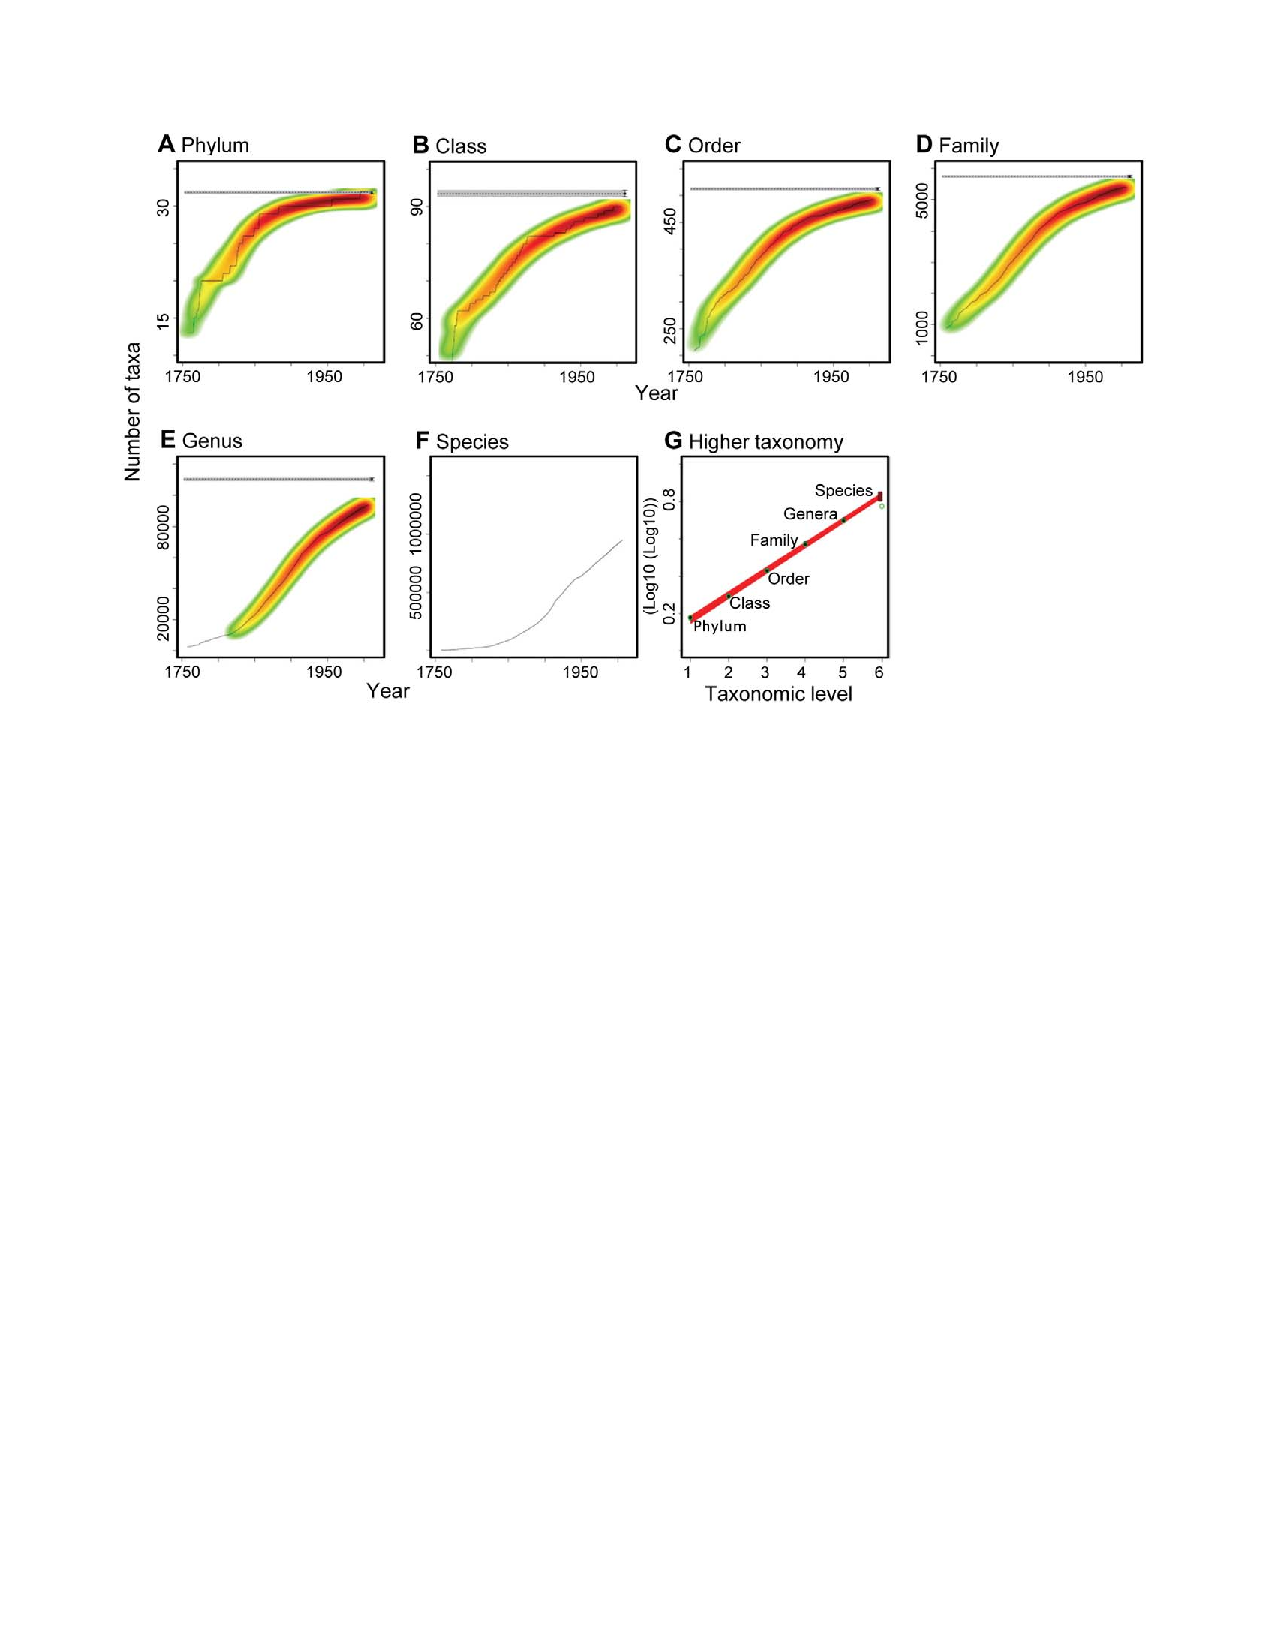
\includegraphics[width=0.8\linewidth]{images/Mora2011} \end{center}

\normalsize

En se limitant aux arbres, l'estimation se monte à 16000 espèces pour l'Amazonie \autocite{TerSteege2013}, de l'ordre de 5000 pour l'Afrique et entre 40000 et 53000 pour l'ensemble des tropiques \autocite{Slik2015} (donc pour l'ensemble de la planète, le nombre d'espèces non-tropicales étant négligeable).
Ces estimations sont obtenues par extrapolation du modèle en log-séries (chapitre \ref{chap-Fisher}) et sont sujettes au paradoxe de Fisher: les espèces représentées par un très petit nombre d'individu dans le modèle, notamment les singletons, sont les plus nombreuses.
Une discussion approfondie est donnée par \textcite{Hubbell2015}: les espèces récemment apparues au sens du modèle ne sont pas détectables avant plusieurs générations, créant un décalage entre le nombre d'espèces reconnues par la taxonomie et le modèle.

\textcite{Wilson2012} compilent les relevés du nombre d'espèces de plantes vasculaires en fonction de la surface et retiennent uniquement les plus riches à chaque échelle spatiale (du millimètre carré à l'hectare).
Ces relevés sont tous situés en forêt tropicale ou en prairie tempérée gérée (les perturbations régulières et modérées y favorisent la diversité, conformément à la théorie de la perturbation intermédiaire \autocite{Connell1978}).
La relation entre le nombre d'espèces et la surface est celle d'Arrhenius.
Son extrapolation à la surface terrestre donne environ 220000 espèces, comparables à l'estimation de 275000 espèces rapportée par Mora et al.

\hypertarget{indice-de-simpson}{%
\section{Indice de Simpson}\label{indice-de-simpson}}

\hypertarget{duxe9finition}{%
\subsection{Définition}\label{duxe9finition}}

On note \(p_s\) la probabilité qu'un individu tiré au hasard appartienne à l'espèce \(s\).
L'indice de \textcite{Simpson1949}, ou Gini-Simpson, est

\begin{equation}
  \label{eq:SimpsonE}
  E = 1 - \sum^{S}_{s=1}{p^2_s}.
\end{equation}

Il peut être interprété comme la probabilité que deux individus tirés au hasard soient d'espèces différentes.
Il est compris dans l'intervalle \(\left[ 0 ; 1 \right[\).
Sa valeur diminue avec la régularité de la distribution: \(E=0\) si une seule espèce a une probabilité de 1, \(E = 1 - 1 / S\) si les \(S\) espèces ont la même probabilité \(p_s = 1 / S\).
La valeur 1 est atteinte pour un nombre infini d'espèces, de probabilités nulles.

Deux autres formes de l'indice sont utilisées.
Tout d'abord, la probabilité que deux individus soient de la même espèce, souvent appelée \emph{indice de concentration de Simpson}, qui est celui défini dans l'article original de Simpson:

\begin{equation}
  \label{eq:SimpsonD}
  D = \sum^{S}_{s=1}{p^2_s}.
\end{equation}

L'indice de Simpson est parfois considéré comme une mesure d'équitabilité \autocite{Olszewski2004} mais il varie avec la richesse: cette approche est donc erronée.
\textcite{Hurlbert1971} l'a divisé par sa valeur maximale \(1 - 1 / S\) pour obtenir une mesure d'équitabilité valide généralisée plus tard par \textcite{Mendes2008}, voir section \ref{sec-Mendes}.
Le nombre d'espèces doit être estimé par les méthodes présentées plus haut, pour ne pas dépendre de la taille de l'échantillon.

L'estimateur du maximum de vraisemblance de l'indice est

\begin{equation}
  \label{eq:EstEML}
  \hat{E} = 1 - \sum^{f_{>0}}_{s=1}{\hat{p}^2_s}.
\end{equation}

Le calcul de l'indice de Simpson peut se faire avec la fonction \texttt{diversity} disponible dans le package \emph{vegan} de R ou avec la fonction \texttt{ent\_simpson} du package \emph{divent}, qui peut traiter plusieurs sites en même temps:

\scriptsize

\begin{Shaded}
\begin{Highlighting}[]
\NormalTok{paracou\_6\_abd }\SpecialCharTok{\%\textgreater{}\%} 
  \CommentTok{\# Transformation des abondances en probabilités}
  \FunctionTok{as\_probabilities}\NormalTok{() }\SpecialCharTok{\%\textgreater{}\%} 
  \FunctionTok{ent\_simpson}\NormalTok{()}
\end{Highlighting}
\end{Shaded}

\begin{verbatim}
## # A tibble: 4 x 5
##   site      weight estimator order entropy
##   <chr>      <dbl> <chr>     <dbl>   <dbl>
## 1 subplot_1   1.56 naive         2   0.975
## 2 subplot_2   1.56 naive         2   0.976
## 3 subplot_3   1.56 naive         2   0.978
## 4 subplot_4   1.56 naive         2   0.971
\end{verbatim}

\normalsize

Un historique de la définition de l'indice, de \textcite{Gini1912} à Simpson, inspiré par Turing, est fourni par Ellerman \autocite*{Ellerman2013}.

\hypertarget{estimation}{%
\subsection{Estimation}\label{estimation}}

Définissons l'indicatrice \({{\mathbf 1}}_{sh}\) valant 1 si l'individu \(h\) appartient à l'espèce \(s\), 0 sinon.
\({{\mathbf 1}}_{sh}\) suit une loi de Bernoulli d'espérance \(p_s\) et de variance \(p_s \left( 1 - p_s \right)\).
\(E\) est la somme sur toutes les espèces de cette variance.
Un estimateur non biaisé d'une variance à partir d'un échantillon est la somme des écarts quadratiques divisée par le nombre d'observation moins une.
L'estimateur \(\hat{E}\) est légèrement biaisé parce qu'il est calculé à partir des \({\hat{p}}_s\), ce qui revient à diviser la somme des écarts par \(n\), et non \(n-1\).
Un estimateur non biaisé est \autocite{Good1953,Lande1996}

\begin{equation} 
  \label{eq:BiaisSimpson}
  \tilde{E} 
  = \left( \frac{n}{n-1} \right) \left( 1 - \sum^{f_{>0}}_{s=1}{{\hat{p}}^2_s} \right).
\end{equation}

La correction par \(n / (n - 1)\) tend rapidement vers 1 quand la taille de l'échantillon augmente: l'estimateur est très peu biaisé.

Le non-échantillonnage des espèces rares est pris en compte dans cette correction parce qu'elle considère que \(\tilde{E}\) est l'estimateur de variance d'un échantillon et non d'une population complètement connue.
Il est négligeable: si \(p_s\) est petit, \(p^2_s\) est négligeable dans la somme.

Simpson a fourni un estimateur non biaisé de \(D\), à partir du calcul du nombre de paires d'individus tirés sans remise:

\begin{equation}
  \label{eq:EstSimpson1949}
  \tilde{D} 
  = \frac{\sum^{S}_{s=1}{n_s \left( n_s - 1 \right)}}{n \left( n - 1 \right)}.
\end{equation}

L'argumentation est totalement différente, mais le résultat est le même: \(\tilde{E}=1-\tilde{D}\).

La fonction \texttt{ent\_simpson} de \emph{divent} accepte comme argument un vecteur d'abondances ou un dataframe contenant les données et propose par défaut la correction de Lande:

\scriptsize

\begin{Shaded}
\begin{Highlighting}[]
\NormalTok{paracou\_6\_abd }\SpecialCharTok{\%\textgreater{}\%} 
  \FunctionTok{ent\_simpson}\NormalTok{()}
\end{Highlighting}
\end{Shaded}

\begin{verbatim}
## # A tibble: 4 x 5
##   site      weight estimator order entropy
##   <chr>      <dbl> <chr>     <dbl>   <dbl>
## 1 subplot_1   1.56 Lande         2   0.976
## 2 subplot_2   1.56 Lande         2   0.978
## 3 subplot_3   1.56 Lande         2   0.980
## 4 subplot_4   1.56 Lande         2   0.972
\end{verbatim}

\normalsize

\hypertarget{indice-de-shannon}{%
\section{Indice de Shannon}\label{indice-de-shannon}}

\hypertarget{duxe9finition-1}{%
\subsection{Définition}\label{duxe9finition-1}}

L'indice de Shannon \autocite{Shannon1948,Shannon1963}, aussi appelé indice de Shannon-Weaver ou Shannon-Wiener \autocite{Spellerberg2003}, ou simplement \emph{entropie} est dérivé de la théorie de l'information:

\begin{equation}
  \label{eq:Shannon}
  H = -\sum^S_{s=1}{p_s\ln{p_s}}.
\end{equation}

Considérons une placette forestière contenant \(S\) espèces végétales différentes.
La probabilité qu'une plante choisie au hasard appartienne à l'espèce \(s\) est notée \(p_s\).
On prélève \(n\) plantes, et on enregistre la liste ordonnée des espèces des \(n\) plantes.
Si \(n\) est suffisamment grand, le nombre de plantes de l'espèce \(s\) est \(np_s\).
On note \(L\) le nombre de listes respectant ces conditions:

\begin{equation}
  \label{eq:ShannonL}
  L = \frac{n!}{\prod^S_{i=1}{\left( {np}_s \right)!}}.
\end{equation}

Ce résultat est obtenu en calculant le nombre de positions possibles dans la liste pour les individus de la première espèce: \(\binom{n}{np_1}\).
Le nombre de positions pour la deuxième espèce est \(\binom{n-np_1}{np_2}\).
Pour la \(S\)-ième espèce, le nombre est \(\binom{n-np_1-\dots -np_{s-1}}{np_i}\).
Les produits de combinaisons se simplifient pour donner l'équation \eqref{eq:ShannonL}.

On peut maintenant écrire le logarithme de \(L\):
\[\ln{L} = \ln{n!} - \sum^S_{s=1}{\ln{np_s}!}.\]
On utilise l'approximation de Stirling,
\[\ln{n!} \approx n \ln{n} - n,\]
pour obtenir après simplifications:

\begin{equation}
  \label{eq:ShannonlnL}
  \ln{L} = -n \sum^S_{s=1}{p_s \ln{p_s}}.
\end{equation}

\(H = (\ln{L}) / n\) est l'indice de Shannon.
Ce résultat est connu sous le nom de formule de \textcite{Brillouin1962}.
À l'origine, Shannon a utilisé un logarithme de base 2 pour que \(H\) soit le nombre moyen de questions binaires (réponse oui ou non) nécessaire pour identifier l'espèce d'une plante (un caractère utilisé dans une chaîne dans le contexte du travail de Shannon).
Les logarithmes naturels, de base 2 ou 10 ont été utilisés par la suite \autocite{Pielou1966a}.

La formule \eqref{eq:ShannonlnL} est celle de l'indice de \textcite{Theil1967}, présenté en détail par \textcite{Conceicao2000}, à l'origine utilisé pour mesurer les inégalités de revenu puis pour caractériser les structures spatiales en économie.
L'indice est proportionnel au nombre de plantes choisies, on peut donc le diviser par \(n\) et on obtient l'indice de biodiversité de Shannon.
Ces indices ont été définis en choisissant des lettres au hasard pour former des chaînes de caractères.
Leur valeur est le nombre de chaînes de caractères différentes que l'on peut obtenir avec l'ensemble des lettres disponibles, c'est-à-dire la quantité d'information contenue dans l'ensemble des lettres.
L'indice de Shannon donne une mesure de la biodiversité en tant que quantité d'information.

L'estimateur du maximum de vraisemblance de l'indice est

\begin{equation}
  \label{eq:EstShannonML}
  \hat{H} = -\sum^{f_{>0}}_{s=1}{\hat{p}_s \ln{\hat{p}_s}}.
\end{equation}

Le calcul de l'indice de Shannon peut se faire avec la fonction \texttt{diversity} disponible dans le package \emph{vegan} de R ou avec la fonction \texttt{ent\_shannon} de \emph{divent}:

\scriptsize

\begin{Shaded}
\begin{Highlighting}[]
\NormalTok{bci\_abd }\SpecialCharTok{\%\textgreater{}\%} 
  \FunctionTok{as\_probabilities}\NormalTok{() }\SpecialCharTok{\%\textgreater{}\%} 
  \FunctionTok{ent\_shannon}\NormalTok{()}
\end{Highlighting}
\end{Shaded}

\begin{verbatim}
## # A tibble: 1 x 5
##   site           weight estimator order entropy
##   <chr>           <dbl> <chr>     <dbl>   <dbl>
## 1 site_707269321      1 naive         1    4.27
\end{verbatim}

\normalsize

La distribution de l'estimateur est connue \autocite{Hutcheson1970} mais elle est inutile en pratique à cause du biais d'estimation.

\textcite{Bulmer1974} établit une relation entre l'indice de Shannon et l'indice \(\alpha\) de Fisher, à condition que la distribution de l'abondance des espèces soit log-normale:

\begin{equation}
  \label{eq:Bulmer1974}
  \hat{H} 
  = \mathrm{\Psi} \left( \hat{\alpha} + 1 \right) - \mathrm{\Psi} \left( 1 \right).
\end{equation}

\(\mathrm{\Psi}(\cdot)\) est la fonction digamma, et \(\hat{\alpha}\) est l'estimateur de l'indice de Fisher \eqref{eq:AlphaFisher}:

\scriptsize

\begin{Shaded}
\begin{Highlighting}[]
\FunctionTok{digamma}\NormalTok{(}\FunctionTok{fisher.alpha}\NormalTok{(}\FunctionTok{colSums}\NormalTok{(BCI)) }\SpecialCharTok{+} \DecValTok{1}\NormalTok{) }\SpecialCharTok{{-}} \FunctionTok{digamma}\NormalTok{(}\DecValTok{1}\NormalTok{)}
\end{Highlighting}
\end{Shaded}

\begin{verbatim}
## [1] 4.148322
\end{verbatim}

\normalsize

La sous-estimation est assez sévère sur cet exemple.

\hypertarget{sec-BiaisShannon}{%
\subsection{Estimation}\label{sec-BiaisShannon}}

\textcite{Basharin1959} a montré que l'estimateur naïf de l'indice de Shannon était biaisé parce que des espèces ne sont pas échantillonnées.
Si \(S\) est le nombre d'espèces réel et \(n\) le nombre d'individus échantillonnés, le biais est

\begin{equation}
  \label{eq:Basharin1959}
  \mathbb{E}\left( \hat{H} \right) - H 
  = -\frac{S - 1}{2n} + O\left(n^{-2}\right).
\end{equation}

\(O(n^{-2})\) est un terme négligeable.
La valeur estimée à partir des données est donc trop faible, d'autant plus que le nombre d'espèces total est grand mais d'autant moins que l'échantillonnage est important.
Comme le nombre d'espèces \(S\) n'est pas observable, le biais réel est inconnu.

L'estimateur de Miller-Madow \autocite{Miller1955} utilise l'information disponible, en sous-estimant le nombre d'espèces et donc l'entropie:
\begin{equation}
  \label{eq:MillerMadow}
  \tilde{H} = -\sum^{f_{>0}}_{s=1}{\hat{p}_s \ln{\hat{p}_s}} + \frac{f_{>0} - 1}{2n}.
\end{equation}

\textcite{Chao2003} établissent un estimateur moins biaisé à partir du taux de couverture de l'échantillonnage \(\hat{C}\):

\begin{equation}
  \label{eq:ChaoShen}
  \tilde{H} 
  = -\sum_{s=1}^{f_{>0}}{\frac
    {\hat{C} \hat{p}_s \ln\left( \hat{C} \hat{p}_s \right)}
    {1 - \left( 1 - \hat{C}\hat{p}_s \right)^n}}.
\end{equation}

Multiplier les fréquences observées par le taux de couverture permet d'obtenir un estimateur non biaisé des probabilités conditionnellement aux espèces non observées \autocite{Ashbridge2000}.

Le terme au dénominateur est la correction de \textcite{Horvitz1952}: chaque terme de la somme est divisé par la probabilité d'observer au moins une fois l'espèce correspondante.
Il tend vers 1 quand la taille de l'échantillon augmente.

\textcite{Beck2010} montrent que la correction du biais est efficace, même à des niveaux de complétude de l'échantillonnage (voir section \ref{sec-ChoixEstimateur}) très faibles. \textcite{Vu2007} étudient la vitesse de convergence de l'estimateur.

\textcite{Zhang2012} définit l'indice de Simpson généralisé:

\begin{equation}
  \label{eq:zeta}
  \zeta_{u,v} = \sum^S_{s=1}{p^u_s{\left( 1 - p_s \right)}^v},
\end{equation}

où \(\zeta_{u,v}\) est la somme sur toutes les espèces de la probabilité de rencontrer \(u\) fois l'espèce dans un échantillon de taille \(u+v\).
L'indice de Shannon peut s'exprimer en fonction de \(\zeta_{1,v}\):

\begin{equation}
  \label{eq:HzetaInf}
  H = \sum^{\infty}_{v=1}{\frac{1}{v} \zeta_{1,v}}.
\end{equation}

Les premiers termes de la somme, jusqu'à \(v=n-1\) peuvent être estimés à partir des données, les suivants constituent le biais de l'estimateur, qui est calculé en pratique par

\begin{equation}
  \label{eq:Hzetanu}
  H_z 
  = \sum^{n-1}_{v=1}{\frac{1}{v}\left\{
    \frac{n^{v+1}\left[ n - \left(v + 1 \right) \right]!}{n!}
    \sum^{f_{>0}}_{s=1}{p_s \prod^{v-1}_{j=0}{
      \left( 1 - \hat{p}_s - \frac{j}{n} \right)}
    }
  \right\}}.
\end{equation}

\textcite{Zhang2013a} montre que le biais de l'estimateur \(H_z\) est asymptotiquement normal et calcule sa variance.
\textcite{Zhang2013} améliorent l'estimateur en le complétant par un estimateur de son biais, mais les calculs deviennent excessivement complexes.
\textcite{Vinck2012} appliquent la même démarche avec un estimateur bayésien du biais, utilisant un prior aussi plat que possible pour la valeur de l'entropie (et non un prior plat sur les probabilités, qui tire l'estimateur vers l'entropie maximale).
Cet estimateur nécessite de connaître le nombre d'espèces, ce qui empêche son utilisation sur des données d'écologie.

\textcite{Pielou1966} a développé une autre méthode de correction de biais lorsque de nombreux relevés de petite taille sont disponibles.
\(\ln{L}\) est calculé pour un relevé choisi aléatoirement puis les données du premier relevé sont ajoutées à celles d'un autre, puis un autre jusqu'à ce que \(H=(\ln{L}) / n\) n'augmente plus: la diversité augmente dans un premier temps mais se stabilise quand l'effet des espèces ajoutées est compensé par celui de la diminution de l'équitabilité due aux espèces présentes dans tous les relevés.
À partir de ce seuil, l'augmentation de \(\ln{L}\) par individu ajouté est calculée pour chaque relevé supplémentaire.
Son espérance, estimée par sa moyenne calculée en ajoutant tous les relevés disponibles, est \(\tilde{H}\).

\textcite{Chao2013} utilisent l'estimateur de la pente de la courbe de raréfaction, calculé précédemment \autocite{Chao2012b} pour estimer la richesse spécifique, pour fournir un estimateur extrêmement performant:

\begin{align}
  \label{eq:Chao2013}
  \tilde{H}
  = &-\sum_{s=1}^{f_{>0}}
    {\frac{n_s}{n} \left( \mathrm{\Psi}\left( n \right) - \mathrm{\Psi}\left( n_s \right) \right)} \\
    &-\frac{s_{1}}{n} {\left(1 - A \right)}^{1 - n} \left( 
      -\ln\left( A \right) -\sum^{n-1}_{r=1}{\frac{1}{r}{\left( 1 - A \right)}^r} \right
    ),
\end{align}

où \(\mathrm{\Psi}(\cdot)\) est la fonction digamma et \(A\) vaut:

\begin{itemize}
\tightlist
\item
  \(2s_{2} / [(n - 1) s_{1} + 2 s_{2}]\) en présence de singletons et doubletons;
\item
  \(2 / [(n - 1) (s_1 -1) + 2]\) en présence de singletons seulement;
\item
  \(1\) en absence de singletons et doubletons.
\end{itemize}

Enfin, la littérature de physique statistique s'est abondamment intéressée à cette question (\textcite{Bonachela2008} en font une revue).
Le problème traité est la non-linéarité de l'indice de Shannon par rapport aux probabilités qui entraîne un biais d'estimation.
La fonction logarithme fournit un exemple simple: l'espérance de \(\ln(p_s)\) n'est pas le logarithme de l'espérance de \(p_s\) parce que la fonction \(\ln\) est concave.
Chaque estimateur \({\hat{p}}_s\) fluctue autour de \(p_s\) mais vaut \(p_s\) en moyenne.
À cause de la concavité, \(\ln(\hat{p}_s)\) est en moyenne inférieur à \(\ln(p_s)\): cette relation est connue sous le nom d'inégalité de \textcite{Jensen1906}.
L'indice de Shannon est concave (figure \ref{fig:ShannonFig}) donc son estimateur \eqref{eq:Shannon} est biaisé négativement, même sans prendre en considération les espèces non observées.



\scriptsize

\begin{SCfigure}

{\centering 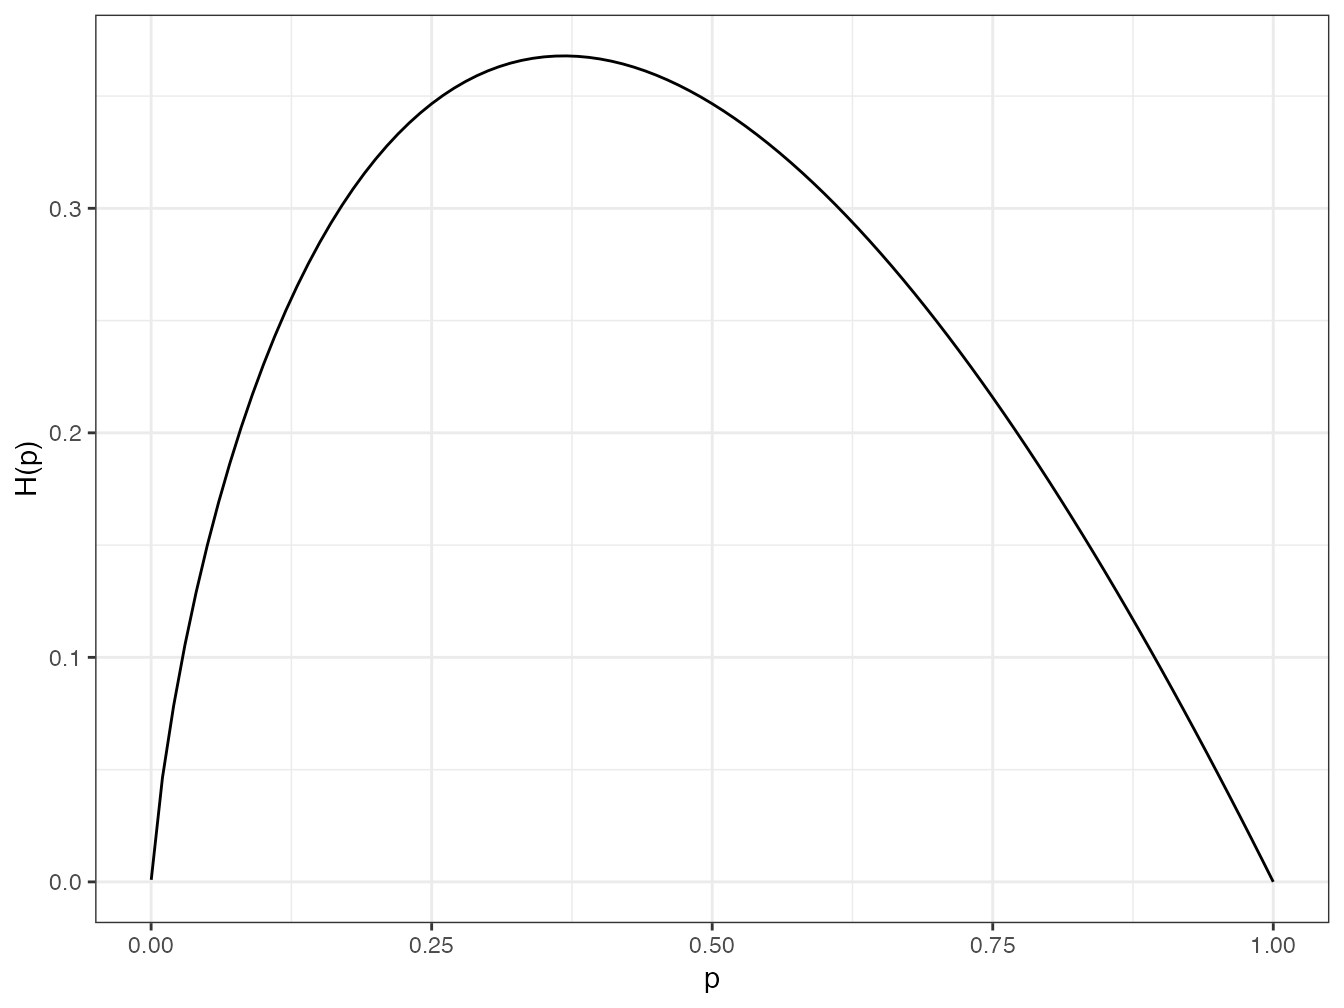
\includegraphics[width=0.8\linewidth]{MesuresBD_files/figure-latex/ShannonFig-1} 

}

\caption{Courbe de \(x\ln x\) entre 0 et 1.}\label{fig:ShannonFig}
\end{SCfigure}

\normalsize

Code de la figure \ref{fig:ShannonFig}:

\scriptsize

\begin{Shaded}
\begin{Highlighting}[]
\FunctionTok{tibble}\NormalTok{(}\AttributeTok{x =} \FunctionTok{c}\NormalTok{(}\FloatTok{0.0001}\NormalTok{, }\DecValTok{1}\NormalTok{)) }\SpecialCharTok{\%\textgreater{}\%} 
  \FunctionTok{ggplot}\NormalTok{(}\FunctionTok{aes}\NormalTok{(x)) }\SpecialCharTok{+} 
    \FunctionTok{stat\_function}\NormalTok{(}\AttributeTok{fun =} \ControlFlowTok{function}\NormalTok{(x) }\SpecialCharTok{{-}}\NormalTok{x }\SpecialCharTok{*} \FunctionTok{log}\NormalTok{(x)) }\SpecialCharTok{+}
    \FunctionTok{labs}\NormalTok{(}\AttributeTok{x =} \StringTok{"p"}\NormalTok{, }\AttributeTok{y =} \StringTok{"H(p)"}\NormalTok{)}
\end{Highlighting}
\end{Shaded}

\normalsize

Le biais peut être évalué par simulation: 10000 tirages sont réalisés dans une loi normale d'espérance \(p_s\) choisie et d'écart-type 0.01.
Le biais est la différence entre \(-p_s \ln{p_s}\) (connu) et la moyenne des 1000 valeurs de \(-\hat{p}_s \ln{\hat{p}}_s\) (la probabilité est estimée par sa réalisation à chaque tirage).
La valeur du biais en fonction de \(p_s\) est en figure \ref{fig:ShannonBiaisFig}.
Le biais de l'indice de Shannon est la somme des biais pour toutes les probabilités spécifiques de la communauté étudiée, et son calcul est toujours l'objet de recherches.



\scriptsize

\begin{SCfigure}

{\centering 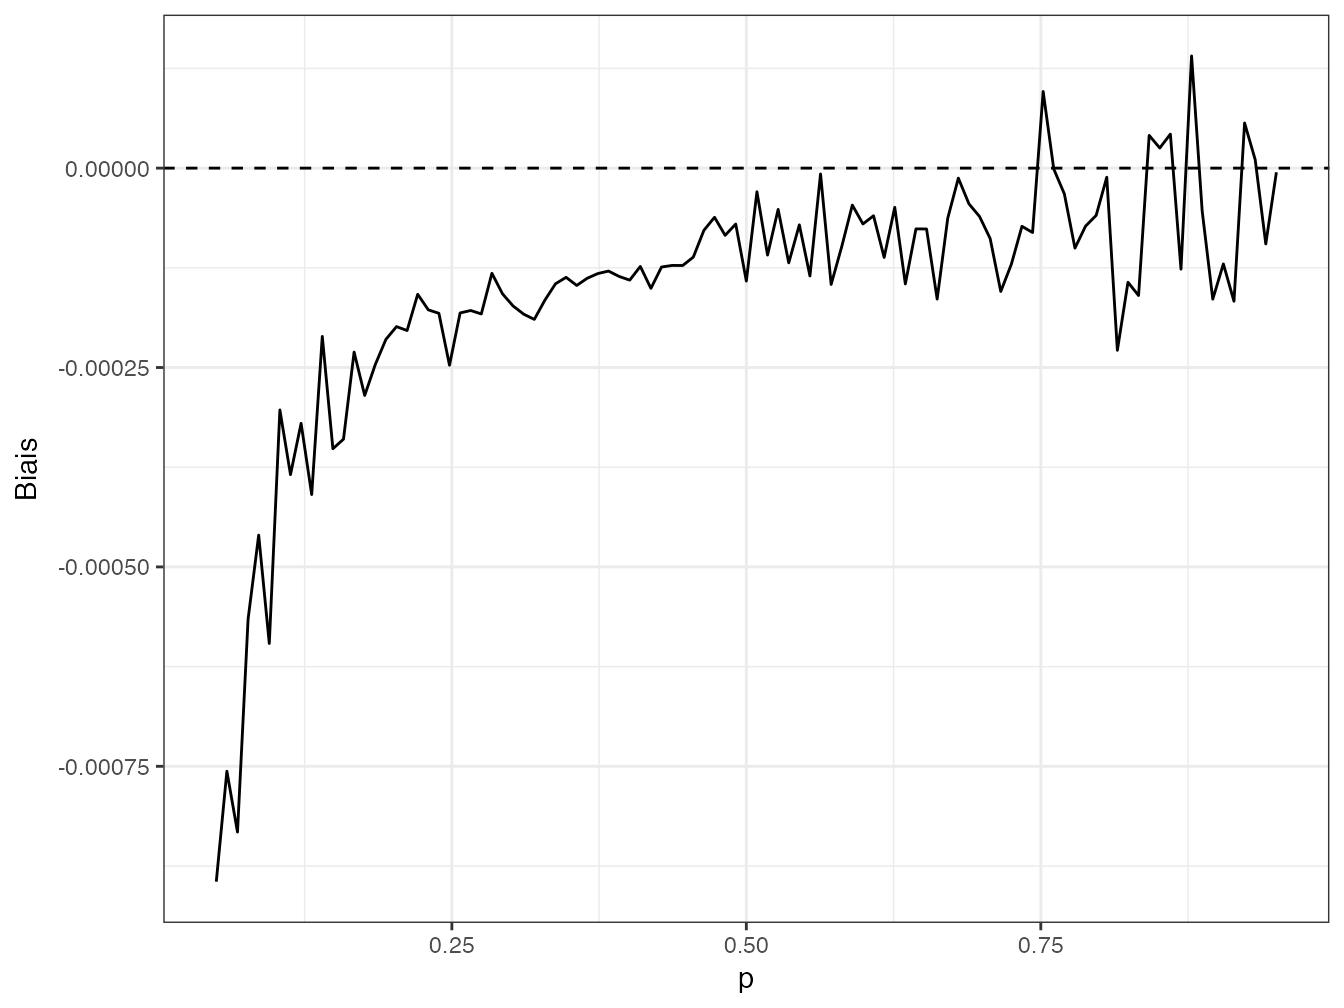
\includegraphics[width=0.8\linewidth]{MesuresBD_files/figure-latex/ShannonBiaisFig-1} 

}

\caption{Biais de \(\hat{p}_s \ln\hat{p}_s\) entre 0 et 1.}\label{fig:ShannonBiaisFig}
\end{SCfigure}

\normalsize

Code de la figure \ref{fig:ShannonBiaisFig}:

\scriptsize

\begin{Shaded}
\begin{Highlighting}[]
\NormalTok{bias\_p }\OtherTok{\textless{}{-}} \ControlFlowTok{function}\NormalTok{ (p) \{}
\NormalTok{  p\_s }\OtherTok{\textless{}{-}}\FunctionTok{rnorm}\NormalTok{(}\DecValTok{10000}\NormalTok{, p, }\FloatTok{0.01}\NormalTok{)}
\NormalTok{  p }\SpecialCharTok{*} \FunctionTok{log}\NormalTok{(p) }\SpecialCharTok{{-}} \FunctionTok{mean}\NormalTok{(p\_s }\SpecialCharTok{*} \FunctionTok{log}\NormalTok{(p\_s))}
\NormalTok{\}}

\NormalTok{bias }\OtherTok{\textless{}{-}} \ControlFlowTok{function}\NormalTok{ (p\_s) \{}
  \CommentTok{\# Applique bias\_p à chaque valeur de p\_s}
  \FunctionTok{sapply}\NormalTok{(p\_s, bias\_p)}
\NormalTok{\}}

\FunctionTok{tibble}\NormalTok{(}\AttributeTok{x =} \FunctionTok{c}\NormalTok{(}\FloatTok{0.05}\NormalTok{, }\FloatTok{0.95}\NormalTok{)) }\SpecialCharTok{\%\textgreater{}\%} 
  \FunctionTok{ggplot}\NormalTok{(}\FunctionTok{aes}\NormalTok{(x)) }\SpecialCharTok{+} 
    \FunctionTok{stat\_function}\NormalTok{(}\AttributeTok{fun =}\NormalTok{ bias) }\SpecialCharTok{+}
    \FunctionTok{geom\_hline}\NormalTok{(}\AttributeTok{yintercept =} \DecValTok{0}\NormalTok{, }\AttributeTok{lty =} \DecValTok{2}\NormalTok{) }\SpecialCharTok{+}
    \FunctionTok{labs}\NormalTok{(}\AttributeTok{x =} \StringTok{"p"}\NormalTok{, }\AttributeTok{y =} \StringTok{"Biais"}\NormalTok{)}
\end{Highlighting}
\end{Shaded}

\normalsize

\textcite{Grassberger1988} a fourni la correction de référence:

\begin{equation}
  \label{eq:Grassberger1988}
  \tilde{H}
  = -\sum^{f_{>0}}_{s=1}{
    \frac{n_s}{n} \left( \ln\left( n \right) - \mathrm{\Psi}\left( n_s \right) 
    -\frac{{\left( -1 \right)}^{n_s}}{n_s + 1} \right)
  }.
\end{equation}

\textcite{Grassberger2003} l'a perfectionnée:

\begin{equation}
  \label{eq:Grassberger2003}
  \tilde{H} 
  = -\sum^{f_{>0}}_{s=1}{
    \frac{n_s}{n} \left( \mathrm{\Psi}\left( n \right) - \mathrm{\Psi}\left( n_s \right)
    -{\left( -1 \right)}^{n_s} \int^1_0{\frac{t^{n_s - 1}}{1 + t} \mathop{dt}} \right)
  }.
\end{equation}

Enfin, \textcite{Schurmann2004} l'a généralisée pour définir une famille de corrections dépendant d'un paramètre \(\xi\):

\begin{equation}
  \label{eq:Schurmann2004}
  \tilde{H} 
  = -\sum^{f_{>0}}_{s=1}{
    \frac{n_s}{n} \left( \mathrm{\Psi}\left( n \right) - \mathrm{\Psi}\left( n_s \right) 
    - {\left( -1 \right)}^{n_s} \int^{\frac{1}{\xi} - 1}_0{\frac{t^{n_s - 1}}{1 + t} \mathop{dt}} \right)
  }.
\end{equation}

Le biais d'estimation diminue avec \(\xi\) mais l'erreur quadratique augmente.
Schürmann suggère d'utiliser \(\xi=e^{-1/2}\) comme meilleur compromis.

La fonction \texttt{ent\_shannon} permet toutes ces corrections.

\scriptsize

\begin{Shaded}
\begin{Highlighting}[]
\FunctionTok{ent\_shannon}\NormalTok{(}\FunctionTok{colSums}\NormalTok{(BCI), }\AttributeTok{estimator =} \StringTok{"ChaoJost"}\NormalTok{)}
\end{Highlighting}
\end{Shaded}

\begin{verbatim}
## # A tibble: 1 x 3
##   estimator order entropy
##   <chr>     <dbl>   <dbl>
## 1 ChaoJost      1    4.28
\end{verbatim}

\begin{Shaded}
\begin{Highlighting}[]
\FunctionTok{ent\_shannon}\NormalTok{(}\FunctionTok{colSums}\NormalTok{(BCI), }\AttributeTok{estimator =} \StringTok{"Grassberger"}\NormalTok{)}
\end{Highlighting}
\end{Shaded}

\begin{verbatim}
## # A tibble: 1 x 3
##   estimator   order entropy
##   <chr>       <dbl>   <dbl>
## 1 Grassberger     1    4.28
\end{verbatim}

\begin{Shaded}
\begin{Highlighting}[]
\FunctionTok{ent\_shannon}\NormalTok{(}\FunctionTok{colSums}\NormalTok{(BCI), }\AttributeTok{estimator =} \StringTok{"Grassberger2003"}\NormalTok{)}
\end{Highlighting}
\end{Shaded}

\begin{verbatim}
## # A tibble: 1 x 3
##   estimator       order entropy
##   <chr>           <dbl>   <dbl>
## 1 Grassberger2003     1    4.28
\end{verbatim}

\begin{Shaded}
\begin{Highlighting}[]
\FunctionTok{ent\_shannon}\NormalTok{(}\FunctionTok{colSums}\NormalTok{(BCI), }\AttributeTok{estimator =} \StringTok{"Schurmann"}\NormalTok{)}
\end{Highlighting}
\end{Shaded}

\begin{verbatim}
## # A tibble: 1 x 3
##   estimator order entropy
##   <chr>     <dbl>   <dbl>
## 1 Schurmann     1    4.28
\end{verbatim}

\begin{Shaded}
\begin{Highlighting}[]
\FunctionTok{ent\_shannon}\NormalTok{(}\FunctionTok{colSums}\NormalTok{(BCI), }\AttributeTok{estimator =} \StringTok{"ZhangHz"}\NormalTok{)}
\end{Highlighting}
\end{Shaded}

\begin{verbatim}
## # A tibble: 1 x 3
##   estimator order entropy
##   <chr>     <dbl>   <dbl>
## 1 ZhangHz       1    4.27
\end{verbatim}

\normalsize

D'autres estimateurs peu utilisés en écologie sont disponibles dans le package \emph{entropy} \autocite{Hausser2009}.
La contraction de Stein \autocite{James1961} consiste à estimer la distribution des probabilités d'occurrence des espèces par la pondération optimale entre un estimateur à faible biais et un estimateur à faible variance.
L'estimateur \(\hat{p}_s\) est sans biais mais a une variance importante.
L'estimateur \(1/S\), si \(S\) est connu, est de variance nulle mais est très biaisé.
Comme le nombre d'espèces est en général inconnu, il doit être estimé par une méthode quelconque, mais de préférence le surestimant plutôt que le sous-estimant.
L'estimateur de James-Stein (\emph{shrinkage estimator}) optimal est
\begin{equation}
  \label{eq:JamesStein1}
  \tilde{p}_s = \hat{\lambda}\frac{1}{\hat{S}} + \left( 1 - \hat{\lambda} \right) \hat{p}_s,
\end{equation}

où
\begin{equation}
  \label{eq:JamesStein2}
  \hat{\lambda} = \frac
    {1 - \sum^{f_{>0}}_{s=1}{\left( \hat{p}_s \right)^2}}
    {\left( n - 1 \right) \sum^{f_{>0}}_{s=1}{\left( \frac{1}{\hat{S}} - \hat{p}_s \right)^2}}.
\end{equation}

L'entropie est ensuite simplement estimée par l'estimateur plug-in: \(\tilde{H} = -\sum^{f_{>0}}_{s=1}{\tilde{p}_s \ln{\tilde{p}_s}}\).
Le calcul sous R est le suivant:

\scriptsize

\begin{Shaded}
\begin{Highlighting}[]
\FunctionTok{library}\NormalTok{(}\StringTok{"entropy"}\NormalTok{)}
\FunctionTok{entropy.shrink}\NormalTok{(}\FunctionTok{colSums}\NormalTok{(BCI))}
\end{Highlighting}
\end{Shaded}

\begin{verbatim}
## Estimating optimal shrinkage intensity lambda.freq (frequencies): 0.0021
\end{verbatim}

\begin{verbatim}
## [1] 4.275689
## attr(,"lambda.freqs")
## [1] 0.002074043
\end{verbatim}

\normalsize

Le principe même de l'estimation rapproche la distribution de l'équiprobabilité des espèces et donc augmente l'entropie.
L'estimation précédente ignore les espèces non observées.
Pour les inclure, le vecteur des abondance doit être allongé par autant de zéros que d'espèces estimées:

\scriptsize

\begin{Shaded}
\begin{Highlighting}[]
\FunctionTok{entropy.shrink}\NormalTok{(}\FunctionTok{c}\NormalTok{(}\FunctionTok{colSums}\NormalTok{(BCI), }\FunctionTok{rep}\NormalTok{(}\DecValTok{0}\NormalTok{, bci\_f\_0)))}
\end{Highlighting}
\end{Shaded}

\begin{verbatim}
## Estimating optimal shrinkage intensity lambda.freq (frequencies): 0.002
\end{verbatim}

\begin{verbatim}
## [1] 4.276543
## attr(,"lambda.freqs")
## [1] 0.002041748
\end{verbatim}

\normalsize

Les fréquences sont estimées par la fonction \texttt{freqs.shrink}.
Leur utilisation dans l'estimateur plug-in donne le même résultat:

\scriptsize

\begin{Shaded}
\begin{Highlighting}[]
\FunctionTok{ent\_shannon}\NormalTok{(}\FunctionTok{freqs.shrink}\NormalTok{(}\FunctionTok{c}\NormalTok{(}\FunctionTok{colSums}\NormalTok{(BCI), }\FunctionTok{rep}\NormalTok{(}\DecValTok{0}\NormalTok{, bci\_f\_0))))}
\end{Highlighting}
\end{Shaded}

\begin{verbatim}
## Estimating optimal shrinkage intensity lambda.freq (frequencies): 0.002
\end{verbatim}

\begin{verbatim}
## # A tibble: 1 x 3
##   estimator order entropy
##   <chr>     <dbl>   <dbl>
## 1 naive         1    4.28
\end{verbatim}

\normalsize

Appliqué à des données de biodiversité aquatique, l'estimateur de James-Stein obtient de meilleurs résultats que celui de Chao et Shen \autocite{Liu2015} quand l'échantillonnage est réduit.

\hypertarget{sec-Hurlbert}{%
\section{Indice de Hurlbert}\label{sec-Hurlbert}}

\hypertarget{duxe9finition-2}{%
\subsection{Définition}\label{duxe9finition-2}}

L'indice de \textcite{Hurlbert1971} est l'espérance du nombre d'espèces observées dans un échantillon de taille \(k\) choisie:

\begin{equation}
  \label{eq:HurlbertSk}
  _{k}S = \sum^S_{s=1}{\left[ 1 - {\left( 1 - p_s \right)}^k \right]}.
\end{equation}

Chaque terme de la somme est la probabilité d'observer au moins une fois l'espèce correspondante.

L'augmentation de la valeur de \(k\) permet de donner plus d'importance aux espèces rares.

L'indice peut être converti en nombre équivalent d'espèces \autocite{Dauby2012}, c'est-à-dire le nombre d'espèces équiprobables nécessaire pour obtenir la même diversité, notés \(_{k}D\) à partir de la relation

\begin{equation}
  \label{eq:HurlbertD}
  _{k}S = {_{k}D} \left[ 1 - {\left( 1 - \frac{1}{_{k}D} \right)}^k \right].
\end{equation}

L'équation doit être résolue pour obtenir \(_{k}D\) à partir de la valeur de \(_{k}S\) estimée, numériquement pour \(k>3\).

Dans deux cas particuliers, les nombres équivalents d'espèces de Hurlbert sont identiques aux nombres de Hill: \(_{2}D = {^{2}\!D}\) et \(_{\infty}D = {^{0}\!D}\).

Pour les autres ordres entiers de diversité, il existe une correspondance parfaite entre les deux mesures \autocite[Annexe S2]{Chao2014}: la connaissance de l'une permet d'obtenir l'autre. Pour \(k>1\), on a \autocite{Leinster2012}

\begin{equation}
  \label{eq:HurlbertDq}
  _{k}S = k + \sum_{q=2}^{k}{\binom{k}{q} \left( -1 \right)^{q + 1} \left( ^{q}\!D \right)^{1-q}}.
\end{equation}

On a vu que \(^{0}\!D\) égale \(_{\infty}D\), donc \(_{\infty}S = {^{0}\!D}\) \eqref{eq:HurlbertD}.

Inversement, pour \(q > 1\):

\begin{equation}
  \label{eq:DqHurlbert}
  (^{q}\!D)^{1-q} = q + \sum_{k=2}^{q}{\binom{q}{k} \left( -1 \right)^{k + 1} {_{k}S}}.
\end{equation}

Pour \(q=1\), la relation est \autocite{Mao2007}
\begin{equation}
  \label{eq:Mao2007}
  ^{1}\!H = -1 + \sum_{k=2}^{\infty}{\frac{_{k}S}{k \left( k - 1 \right)}}.
\end{equation}

\hypertarget{estimation-1}{%
\subsection{Estimation}\label{estimation-1}}

Hurlbert fournit un estimateur non biaisé de son indice (\(n\) est la taille de l'échantillon, \(n_s\) le nombre d'individus de l'espèce \(s\)):

\begin{equation}
  \label{eq:EstHurlbert}
  _k{\tilde{S}}
  = \sum_{s=1}^{f_{>0}}{\left[ 1-{\binom{n - n_s}{k}}/{\binom{n}{k}} \right]}.
\end{equation}

\textcite{Dauby2012} montrent que cet estimateur est très peu sensible à la taille de l'échantillon, et obtient de meilleurs résultats sur ce point que les estimateurs de Chao et Shen pour l'indice de Shannon ou du nombre d'espèces.
\textcite{Smith1977} ont calculé sa variance.

Le calcul de la diversité de Hurlbert est possible dans \emph{divent}:

\scriptsize

\begin{Shaded}
\begin{Highlighting}[]
\CommentTok{\# Indice de Hurlbert (probabilités)}
\FunctionTok{ent\_hurlbert}\NormalTok{(}\FunctionTok{as\_probabilities}\NormalTok{(}\FunctionTok{colSums}\NormalTok{(BCI)), }\AttributeTok{k =} \DecValTok{2}\NormalTok{)}
\end{Highlighting}
\end{Shaded}

\begin{verbatim}
## # A tibble: 1 x 5
##   site           weight estimator order entropy
##   <chr>           <dbl> <chr>     <dbl>   <dbl>
## 1 site_402217706      1 naive         2    1.97
\end{verbatim}

\begin{Shaded}
\begin{Highlighting}[]
\CommentTok{\# Estimateur sans biais (abondances)}
\FunctionTok{ent\_hurlbert}\NormalTok{(}\FunctionTok{colSums}\NormalTok{(BCI), }\AttributeTok{k =} \DecValTok{2}\NormalTok{)}
\end{Highlighting}
\end{Shaded}

\begin{verbatim}
## # A tibble: 1 x 3
##   estimator order entropy
##   <chr>     <dbl>   <dbl>
## 1 Hurlbert      2    1.97
\end{verbatim}

\begin{Shaded}
\begin{Highlighting}[]
\CommentTok{\# Nombre effectif d\textquotesingle{}espèces}
\FunctionTok{div\_hurlbert}\NormalTok{(}\FunctionTok{colSums}\NormalTok{(BCI), }\AttributeTok{k =} \DecValTok{2}\NormalTok{)}
\end{Highlighting}
\end{Shaded}

\begin{verbatim}
## # A tibble: 1 x 3
##   estimator order diversity
##   <chr>     <dbl>     <dbl>
## 1 Hurlbert      2      38.1
\end{verbatim}

\normalsize

\hypertarget{entropie}{%
\chapter{Entropie}\label{entropie}}

\begin{Summary}
L'entropie est la surprise moyenne apportée par l'observation des individus d'une communauté, d'autant plus grande qu'un individu appartient à une espèce plus rare.
L'entropie HCDT permet d'unifier les indices classiques de diversité: son paramètre, appelé ordre, fixe l'importance donnée aux espèces rares. L'entropie d'ordre 0 est la richesse; celle d'ordre 1, l'indice de Shannon; celle d'ordre 2, celui de Simpson.
L'entropie est la moyenne du logarithme déformé de la rareté des espèces, définie comme l'inverse de leur probabilité.

L'entropie va de pair avec la diversité au sens strict (Nombres de Hill): le nombre d'espèces équiprobables dont l'entropie est la même que celle de la communauté réelle.
La diversité est l'exponentielle déformée de l'entropie.
Les profils de diversité représentent la diversité en fonction de son ordre et permettent la comparaison de communautés.

L'estimation de la diversité est difficile pour des ordres inférieurs à \(0,5\) dans des taxocènes très divers comme les arbres des forêts tropicales.

\end{Summary}

L'entropie peut être entendue comme la surprise moyenne fournie par l'observation d'un échantillon.
C'est intuitivement une bonne mesure de diversité \autocite{Pielou1975}.
Ses propriétés mathématiques permettent d'unifier les mesures de diversité dans un cadre général.

\hypertarget{duxe9finition-de-lentropie}{%
\section{Définition de l'entropie}\label{duxe9finition-de-lentropie}}

Les textes fondateurs sont \textcite{Davis1941} et surtout \textcite{Theil1967} en économétrie, et Shannon \autocite*{Shannon1948,Shannon1963} pour la mesure de la diversité.
Une revue est fournie par \textcite{Maasoumi1993}.

Considérons une expérience dont les résultats possibles sont \(\{r_1, r_2, \dots , \ r_S\}\).
La probabilité d'obtenir \(r_s\) est \(p_s\), et \(\mathbf{p}=(p_1, p_2, \dots, p_S)\) est le vecteur composé des probabilités d'obtenir chaque résultat.
Les probabilités sont connues \emph{a priori}.
Tout ce qui suit est vrai aussi pour des valeurs de \(r\) continues, dont on connaîtrait la densité de probabilité.

On considère maintenant un échantillon de valeurs de \(r\).
La présence de \(r_s\) dans l'échantillon est peu étonnante si \(p_s\) est grande: elle apporte peu d'information supplémentaire par rapport à la simple connaissance des probabilités.
En revanche, si \(p_s\) est petite, la présence de \(r_s\) est surprenante.
On définit donc une fonction d'information, \(I(p_s)\), décroissante quand la probabilité augmente, de \(I(0) > 0\) (éventuellement \(+\infty\)) à \(I(1) = 0\), parce qu'observer un résultat certain n'apporte aucune information.
Chaque valeur observée dans l'échantillon apporte une certaine quantité d'information, dont la somme est l'information de l'échantillon.
\textcite{Patil1982} appellent l'information \enquote{rareté}.

La quantité d'information attendue de l'expérience est \(\sum^S_{s=1}{p_s I(p_s) = H(\mathbf{p})}\).
Si on choisit \(I(p_s) = -\ln(p_s)\), \(H(\mathbf{p})\) est l'indice de Shannon, mais bien d'autres formes de \(I(p_s)\) sont possibles.
\(H(\mathbf{p})\) est appelée \emph{entropie}.
C'est une mesure de l'incertitude (de la volatilité) du résultat de l'expérience.
Si le résultat est certain (une seule valeur \(p_S\) vaut 1), l'entropie est nulle.
L'entropie est maximale quand les résultats sont équiprobables.

Si \(\mathbf{p}\) est la distribution des probabilité des espèces dans une communauté, \textcite{Patil1982} montrent que:

\begin{itemize}
\tightlist
\item
  Si \(I(p_s) = (1 - p_s) / {p_s}\), alors \(H(\mathbf{p})\) est le nombre d'espèces \(S\) moins 1;
\item
  Si \(I(p_s) = -\ln(p_s)\), alors \(H(\mathbf{p})\) est l'indice de Shannon;
\item
  Si \(I(p_s) = 1 - p_s\), alors \(H(\mathbf{p})\) est l'indice de Simpson.
\end{itemize}



\scriptsize

\normalsize

Ces trois fonctions d'information sont représentées en figure \ref{fig:IFig}.

Le code R nécessaire pour réaliser la figure est:

\scriptsize

\begin{Shaded}
\begin{Highlighting}[]
\NormalTok{I0 }\OtherTok{\textless{}{-}} \ControlFlowTok{function}\NormalTok{(p) (}\DecValTok{1}\SpecialCharTok{{-}}\NormalTok{ p) }\SpecialCharTok{/}\NormalTok{ p}
\NormalTok{I1 }\OtherTok{\textless{}{-}} \ControlFlowTok{function}\NormalTok{(p) }\SpecialCharTok{{-}}\FunctionTok{log}\NormalTok{(p)}
\NormalTok{I2 }\OtherTok{\textless{}{-}} \ControlFlowTok{function}\NormalTok{(p) }\DecValTok{1} \SpecialCharTok{{-}}\NormalTok{ p}
\FunctionTok{tibble}\NormalTok{(}\AttributeTok{x =} \FunctionTok{c}\NormalTok{(}\DecValTok{0}\NormalTok{, }\DecValTok{1}\NormalTok{)) }\SpecialCharTok{\%\textgreater{}\%} 
  \FunctionTok{ggplot}\NormalTok{(}\FunctionTok{aes}\NormalTok{(x)) }\SpecialCharTok{+} 
    \FunctionTok{stat\_function}\NormalTok{(}\AttributeTok{fun =}\NormalTok{ I0) }\SpecialCharTok{+}
    \FunctionTok{stat\_function}\NormalTok{(}\AttributeTok{fun =}\NormalTok{ I1, }\AttributeTok{lty =} \DecValTok{2}\NormalTok{) }\SpecialCharTok{+}
    \FunctionTok{stat\_function}\NormalTok{(}\AttributeTok{fun =}\NormalTok{ I2, }\AttributeTok{lty =} \DecValTok{3}\NormalTok{) }\SpecialCharTok{+}
    \FunctionTok{coord\_cartesian}\NormalTok{(}\AttributeTok{ylim =} \FunctionTok{c}\NormalTok{(}\DecValTok{0}\NormalTok{, }\DecValTok{10}\NormalTok{)) }\SpecialCharTok{+}
    \FunctionTok{labs}\NormalTok{(}\AttributeTok{x =} \StringTok{"p"}\NormalTok{, }\AttributeTok{y =} \StringTok{"I(p)"}\NormalTok{)}
\end{Highlighting}
\end{Shaded}

\normalsize



\scriptsize

\begin{SCfigure}

{\centering 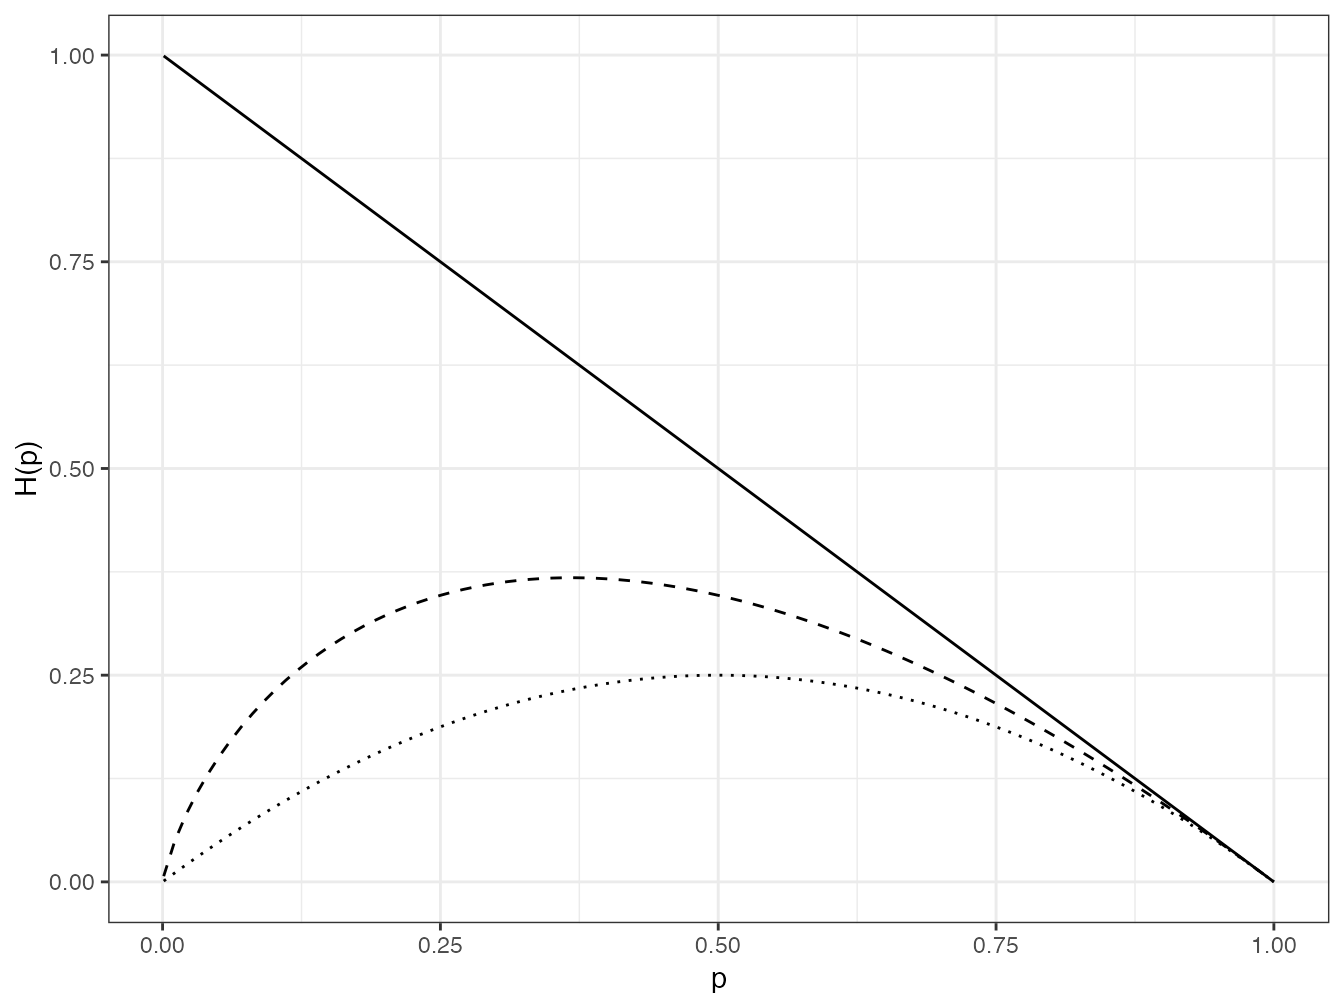
\includegraphics[width=0.8\linewidth]{MesuresBD_files/figure-latex/EntropieFig-1} 

}

\caption{Valeur de \(p_{s}I(p_s)\) dans le nombre d'espèces (trait plein), l'indice de Shannon (pointillés longs) et l'indice de Simpson (pointillés). Les espèces rares contribuent peu, sauf pour le nombre d'espèces.}\label{fig:EntropieFig}
\end{SCfigure}

\normalsize

La contribution de chaque espèce à la valeur totale de l'entropie est représentée figure \ref{fig:EntropieFig}.

Code R:

\scriptsize

\begin{Shaded}
\begin{Highlighting}[]
\NormalTok{H0 }\OtherTok{\textless{}{-}} \ControlFlowTok{function}\NormalTok{(p) }\DecValTok{1} \SpecialCharTok{{-}}\NormalTok{ p}
\NormalTok{H1 }\OtherTok{\textless{}{-}} \ControlFlowTok{function}\NormalTok{(p) }\SpecialCharTok{{-}}\NormalTok{p }\SpecialCharTok{*} \FunctionTok{log}\NormalTok{(p)}
\NormalTok{H2 }\OtherTok{\textless{}{-}} \ControlFlowTok{function}\NormalTok{(p) p }\SpecialCharTok{*}\NormalTok{ (}\DecValTok{1} \SpecialCharTok{{-}}\NormalTok{ p)}
\FunctionTok{tibble}\NormalTok{(}\AttributeTok{x =} \FunctionTok{c}\NormalTok{(}\FloatTok{0.001}\NormalTok{, }\DecValTok{1}\NormalTok{)) }\SpecialCharTok{\%\textgreater{}\%} 
  \FunctionTok{ggplot}\NormalTok{(}\FunctionTok{aes}\NormalTok{(x)) }\SpecialCharTok{+} 
    \FunctionTok{stat\_function}\NormalTok{(}\AttributeTok{fun =}\NormalTok{ H0) }\SpecialCharTok{+}
    \FunctionTok{stat\_function}\NormalTok{(}\AttributeTok{fun =}\NormalTok{ H1, }\AttributeTok{lty =} \DecValTok{2}\NormalTok{) }\SpecialCharTok{+}
    \FunctionTok{stat\_function}\NormalTok{(}\AttributeTok{fun =}\NormalTok{ H2, }\AttributeTok{lty =} \DecValTok{3}\NormalTok{) }\SpecialCharTok{+}
    \FunctionTok{labs}\NormalTok{(}\AttributeTok{x =} \StringTok{"p"}\NormalTok{, }\AttributeTok{y =} \StringTok{"H(p)"}\NormalTok{)}
\end{Highlighting}
\end{Shaded}

\normalsize

\hypertarget{entropie-relative}{%
\section{Entropie relative}\label{entropie-relative}}

Considérons maintenant les probabilités \(q_s\) formant l'ensemble \(\mathbf{q}\) obtenues par la réalisation de l'expérience.
Elles sont différentes des probabilités \(p_s\), par exemple parce que l'expérience ne s'est pas déroulée exactement comme prévu.
On définit le gain d'information \(I(q_s, p_s)\) comme la quantité d'information supplémentaire fournie par l'observation d'un résultat de l'expérience, connaissant les probabilités \emph{a priori}.
La quantité totale d'information fournie par l'expérience, \(\sum^S_{s=1}{q_s I(q_s, p_s)} = H(\mathbf{q}, \mathbf{p})\), est souvent appelée entropie relative.
Elle peut être vue comme une distance entre la distribution \emph{a priori} et la distribution \emph{a posteriori}.
Il est possible que les distributions \(\mathbf{p}\) et \(\mathbf{q}\) soit identiques, que le gain d'information soit donc nul, mais les estimateurs empiriques n'étant pas exactement égaux entre eux, des tests de significativité de la valeur de \(\hat{H}(\mathbf{q},\mathbf{p})\) seront nécessaires.

Quelques formes possibles de \(H(\mathbf{q}, \mathbf{p})\) sont:

\begin{itemize}
\tightlist
\item
  La divergence de Kullback-Leibler \autocite{Kullback1951} connue par les économistes comme l'indice de dissimilarité de \textcite{Theil1967}:
  \begin{equation}
  \label{eq:Theil}
  T = \sum^S_{s=1}{q_{s}\ln\frac{q_s}{p_s}};
  \end{equation}
\item
  Sa proche parente, appelée parfois deuxième mesure de Theil \autocite{Conceicao2000}, qui inverse simplement les rôles de \(p\) et \(q\):
  \begin{equation}
  \label{eq:Theil2}
  L = \sum^S_{s=1}{p_{s}\ln\frac{p_s}{q_s}}.
  \end{equation}
\end{itemize}



\scriptsize

\begin{SCfigure}

{\centering 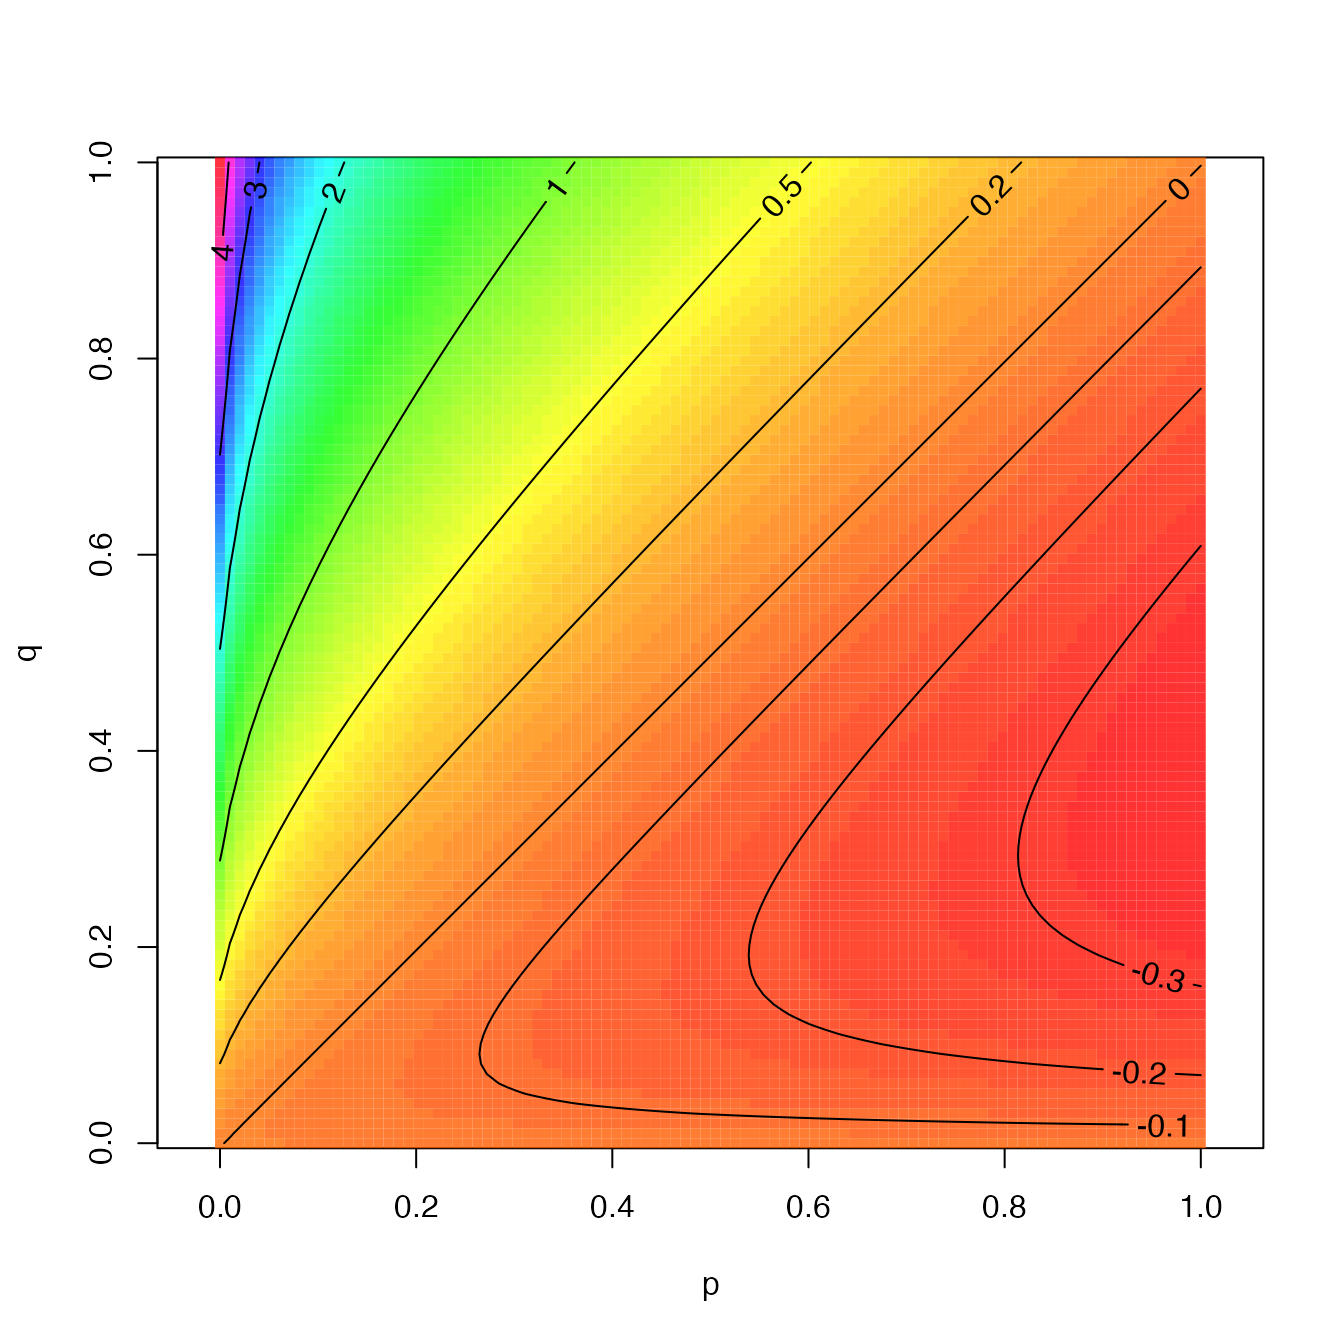
\includegraphics[width=0.8\linewidth]{MesuresBD_files/figure-latex/KullbackLeiblerFig-1} 

}

\caption{Valeur de \(q \ln(q / p)\) en fonction de \(p\) et \(q\). La divergence de Kullback-Leibler est la somme de cette valeur pour toutes les espèces}\label{fig:KullbackLeiblerFig}
\end{SCfigure}

\normalsize

L'entropie relative est essentielle pour la définition de la diversité \(\beta\) présentée dans le chapitre \ref{chap-DedompHCDT}.
En se limitant à la diversité \(\alpha\), on peut remarquer que l'indice de Shannon est la divergence de Kullback-Leibler entre la distribution observée et l'équiprobabilité des espèces \autocite{Marcon2012a}.

La contribution à la divergence de chaque couple \((p_s, q_s)\) est représentées en figure \ref{fig:KullbackLeiblerFig}.
Elle est positive quand \(q_s > p_s\) (la valeur observée est plus grande que la valeur attendue), et croît avec \(q_s\) pour \(p_s\) fixé.
Elle tend vers l'infini quand \(p_s \to 0\).
Les valeurs les plus négatives ne sont pas obtenues pour les valeurs minimales de \(q\) parce que les évènements très rarement observés influent peu sur la quantité d'information totale.
Le minimum \(-e^{-1} \approx 0.37\) est atteint pour \(p_s = 1\) et \(q_s = e^{-1}\), la valeur qui annule la dérivée de \(q \ln(q)\).
En somme, la divergence de Kullback-Leibler est surtout influencée par les évènements beaucoup plus observés qu'attendus.

Le code R nécessaire pour réaliser la figure est:

\scriptsize

\begin{Shaded}
\begin{Highlighting}[]
\NormalTok{p }\OtherTok{\textless{}{-}}\NormalTok{ q }\OtherTok{\textless{}{-}} \FunctionTok{seq}\NormalTok{(}\FloatTok{0.01}\NormalTok{, }\DecValTok{1}\NormalTok{, .}\DecValTok{01}\NormalTok{)}
\NormalTok{KB }\OtherTok{\textless{}{-}} \ControlFlowTok{function}\NormalTok{(p, q) q }\SpecialCharTok{*} \FunctionTok{log}\NormalTok{(q }\SpecialCharTok{/}\NormalTok{ p)}
\NormalTok{xyz }\OtherTok{\textless{}{-}} \FunctionTok{outer}\NormalTok{(p, q, }\AttributeTok{FUN =} \StringTok{"KB"}\NormalTok{)}
\FunctionTok{library}\NormalTok{(}\StringTok{"sp"}\NormalTok{)}
\FunctionTok{image}\NormalTok{(}
\NormalTok{  xyz, }
  \AttributeTok{col =} \FunctionTok{rainbow}\NormalTok{(}\AttributeTok{n =} \DecValTok{100}\NormalTok{, }\AttributeTok{alpha =} \FloatTok{0.8}\NormalTok{), }
  \AttributeTok{xlab =} \StringTok{"p"}\NormalTok{, }
  \AttributeTok{ylab =} \StringTok{"q"}\NormalTok{, }
  \AttributeTok{asp =} \DecValTok{1}
\NormalTok{)}
\FunctionTok{contour}\NormalTok{(}
\NormalTok{  xyz, }
  \AttributeTok{levels =} \FunctionTok{c}\NormalTok{(}\FunctionTok{seq}\NormalTok{(}\SpecialCharTok{{-}}\NormalTok{.}\DecValTok{3}\NormalTok{, }\DecValTok{0}\NormalTok{, .}\DecValTok{1}\NormalTok{), }\FunctionTok{c}\NormalTok{(.}\DecValTok{2}\NormalTok{, .}\DecValTok{5}\NormalTok{), }\FunctionTok{seq}\NormalTok{(}\DecValTok{1}\NormalTok{, }\DecValTok{4}\NormalTok{, }\DecValTok{1}\NormalTok{)), }
  \AttributeTok{labcex =} \DecValTok{1}\NormalTok{, }
  \AttributeTok{add =}\NormalTok{ T}
\NormalTok{)}
\end{Highlighting}
\end{Shaded}

\normalsize

\hypertarget{lappropriation-de-lentropie-par-la-biodiversituxe9}{%
\section{L'appropriation de l'entropie par la biodiversité}\label{lappropriation-de-lentropie-par-la-biodiversituxe9}}

\textcite{MacArthur1955} est le premier à avoir introduit la théorie de l'information en écologie \autocite{Ulanowicz2001}.
MacArthur s'intéressait aux réseaux trophiques et cherchait à mesurer leur stabilité: l'indice de Shannon qui comptabilise le nombre de relations possibles lui paraissait une bonne façon de l'évaluer.
Mais l'efficacité implique la spécialisation, ignorée dans \(H\) qui est une mesure neutre (toutes les espèces y jouent le même rôle).
MacArthur a abandonné cette voie.

Les premiers travaux consistant à généraliser l'indice de Shannon sont dus à \textcite{Renyi1961}.
L'entropie d'ordre \(q\) de Rényi est

\begin{equation}
^{q}\!R =\frac{1}{1 - q \ln\sum^S_{q=1}{p^q_s}}.
\end{equation}

Rényi pose également les axiomes pour une mesure d'entropie \(R(\mathbf{p})\), où \(\mathbf{p}=(p_1, p_2, \dots, p_S)\):

\begin{itemize}
\tightlist
\item
  La symétrie: les espèces doivent être interchangeables, aucune n'a de rôle particulier et leur ordre est indifférent;
\item
  La mesure doit être continue par rapport aux probabilités;
\item
  La valeur maximale est atteinte si toutes les probabilités sont égales.
\end{itemize}

Il montre que \(^{q}\!R\) respecte les 3 axiomes.

\textcite{Patil1982} ont montré de plus que:

\begin{itemize}
\tightlist
\item
  L'introduction d'une espèce dans une communauté augmente sa diversité (conséquence de la décroissance de \(g(p_s)\));
\item
  Le remplacement d'un individu d'une espèce fréquente par un individu d'une espèce plus rare augmente l'entropie à condition que \(R(\mathbf{p})\) soit concave.
  Dans la littérature économique sur les inégalités, cette propriété est connue sous le nom de Pigou-Dalton \autocite{Dalton1920}.
\end{itemize}

\textcite{Hill1973} transforme l'entropie de Rényi en \emph{nombres de Hill}, qui en sont simplement l'exponentielle:

\begin{equation}
  \label{eq:Hill1973}
  ^{q}\!D = {\left(\sum^S_{s=1}{p^q_s}\right)}^{\frac{1}{1 - q}}.
\end{equation}

Le souci de Hill était de rendre les indices de diversité intelligibles après l'article remarqué de \textcite{Hurlbert1971} intitulé \enquote{le non-concept de diversité spécifique}.
Hurlbert reprochait à la littérature sur la diversité sa trop grande abstraction et son éloignement des réalités biologiques, notamment en fournissant des exemples dans lesquels l'ordre des communautés n'est pas le même selon l'indice de diversité choisi.
Les nombres de Hill sont le nombre d'espèces équiprobables donnant la même valeur de diversité que la distribution observée.
Ils sont des transformations simples des indices classiques:

\begin{itemize}
\tightlist
\item
  \(^{0}\!D\) est le nombre d'espèces;
\item
  \(^{1}\!D = e^H\), l'exponentielle de l'indice de Shannon;
\item
  \(^{2}\!D = {1} / {(1- E)}\), l'inverse de l'indice de concentration de Simpson, connu sous le nom d'indice de \textcite{Stoddart1983}.
\end{itemize}

Ces résultats avaient déjà été obtenus avec une autre approche par \textcite{MacArthur1965} et repris par \textcite{Adelman1969} dans la littérature économique.

Les nombres de Hill sont des \enquote{nombres effectifs} ou \enquote{nombres équivalents}.
Le concept a été défini rigoureusement par \textcite{Gregorius1991}, d'après \textcite{Wright1931} (qui avait le premier défini la taille effective d'une population): étant donné une variable caractéristique (ici, l'entropie) fonction seulement d'une variable numérique (ici, le nombre d'espèces), dans un cas idéal (ici, l'équiprobabilité des espèces), le nombre effectif est la valeur de la variable numérique pour laquelle la variable caractéristique est celle du jeu de données.

\textcite{Gregorius2014} montre que de nombreux autres indices de diversité sont acceptables dans le sens où ils vérifient les axiomes précédents et, de plus, que la diversité d'un assemblage de communautés est obligatoirement supérieure à la diversité moyenne de ces communautés (l'égalité n'étant possible que si les communautés sont toutes identiques).
Cette dernière propriété sera traitée en détail dans la partie consacrée à la décomposition de la diversité.
Ces indices doivent vérifier deux propriétés: leur fonction d'information doit être décroissante, et ils doivent être une fonction strictement concave de \(p_s\).
Parmi les possibilités, \(I(p_s) = \cos{(p_s \pi / 2)}\) est envisageable par exemple: le choix de la fonction d'information est virtuellement illimité, mais seules quelques unes seront interprétables clairement.

Un nombre équivalent d'espèces existe pour tous ces indices, il est toujours égal à l'inverse de l'image de l'indice par la réciproque de la fonction d'information:

\begin{equation}
  \label{eq:Gregorius2014}
  D = \frac{1}{I^{-1} \left( \sum^S_{s=1}{p_s I(p_s)} \right)}.
\end{equation}

D'autres entropies ont été utilisées, avec plus ou moins de succès.
Par exemple, \textcite{Ricotta2003c} proposent d'utiliser la fonction d'information \(I(p_s) = -\ln(k_s)\) où \(k_s\) est la dissimilarité totale de l'espèce \(s\) avec les autres (par exemple, la somme des distances aux autres espèces dans un arbre phylogénétique, voir section \ref{sec-Dphylo}), normalisée pour que \(\sum_s{k_s} = 1\).
Ainsi, les espèces les plus originales apportent peu d'information, ce qui n'est pas très intuitif.
Les auteurs montrent que leur mesure est la somme de l'entropie de Shannon et de la divergence de Kullback-Leibler entre les probabilités et les dissimilarités des espèces.
\textcite{Ricotta2006b} ont défini plus tard une entropie augmentant avec l'originalité de chaque espèce, présentée au chapitre \ref{chap-LeinsterCobbold}.

\hypertarget{entropie-hcdt}{%
\section{Entropie HCDT}\label{entropie-hcdt}}

\textcite{Tsallis1988} propose une classe de mesures appelée entropie généralisée, définie par \textcite{Havrda1967} pour la première fois et redécouverte plusieurs fois, notamment par \textcite{Daroczy1970}, d'où son nom \emph{entropie HCDT} (voir \textcite{Mendes2008}, page 451, pour un historique complet):

\begin{equation}
  \label{eq:HCDT}
  ^{q}\!H = \frac{1}{q-1} \left( 1 - \sum^S_{s=1}{p^q_s} \right).
\end{equation}

Tsallis a montré que les indices de Simpson et de Shannon étaient des cas particuliers d'entropie généralisée, retrouvant, sans faire le rapprochement \autocite{Ricotta2005}, la définition d'un indice de diversité de \textcite{Patil1982}.

Ces résultats ont été complétés par d'autres et repris en écologie par \textcite{Keylock2005} et Jost \autocite*{Jost2006,Jost2007}.
Là encore:

\begin{itemize}
\tightlist
\item
  Le nombre d'espèces moins 1 est \(^{0}\!H\);
\item
  L'indice de Shannon est \(^{1}\!H\);
\item
  L'indice de Gini-Simpson est \(^{2}\!H\).
\end{itemize}

L'entropie HCDT est particulièrement attractive parce que sa relation avec la diversité au sens strict est simple, après introduction du formalisme adapté (les logarithmes déformés).
Son biais d'estimation peut être corrigé globalement, et non seulement pour les cas particuliers (nombre d'espèces, Shannon, Simpson).
Enfin, sa décomposition sera présentée en détail dans le chapitre \ref{chap-DedompHCDT}.

\hypertarget{logarithmes-duxe9formuxe9s}{%
\section{Logarithmes déformés}\label{logarithmes-duxe9formuxe9s}}

L'écriture de l'entropie HCDT est largement simplifiée en introduisant le formalisme des logarithmes déformés \autocite{Tsallis1994}.
Le logarithme d'ordre \(q\) est défini par
\begin{equation}
  \label{eq:lnq}
  \ln_q{x} = \frac{x^{1-q} - 1}{1 - q},
\end{equation}
dont la forme est identique à la transformation de \textcite{Box1964} utilisée en statistiques pour normaliser une variable.

Le logarithme déformé converge vers le logarithme naturel quand \(q \to 1\) (figure \ref{fig:lnqFig}).



\scriptsize

\begin{SCfigure}

{\centering 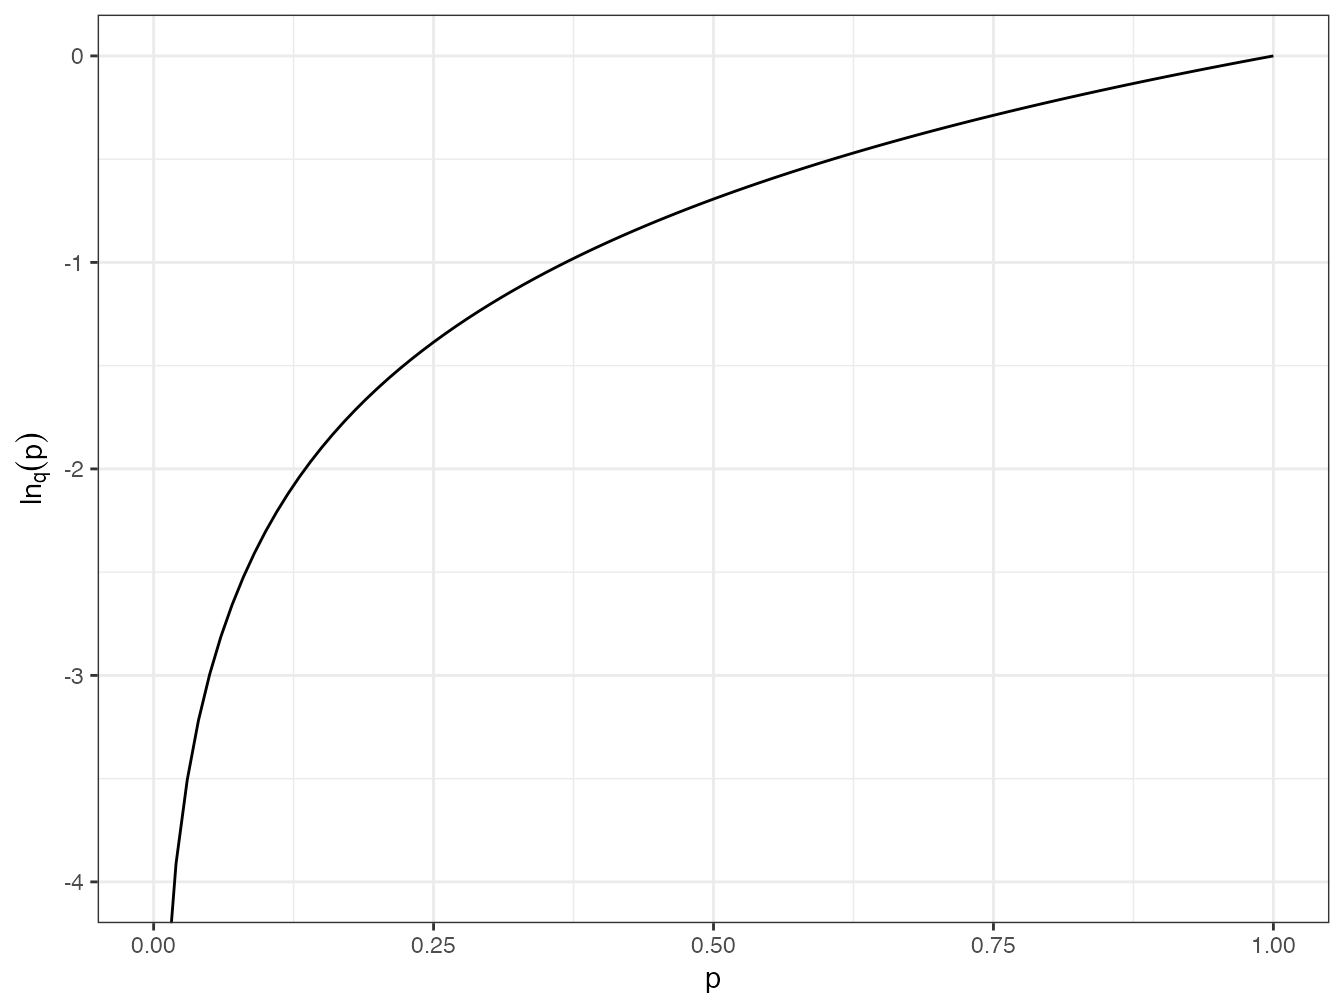
\includegraphics[width=0.8\linewidth]{MesuresBD_files/figure-latex/lnqFig-1} 

}

\caption{Valeur du logarithme d'ordre \(q\) de probabilités entre 0 et 1 pour différentes valeurs de \(q\): \(q = 0\) (pointillés longs rouges), la courbe est une droite; \(q = 1\) (trait plein): logarithme naturel; \(q = 2\) (pointillés courts bleus): la courbe a la même forme que le logarithme naturel pour les valeurs positives de \(q\); \(q = -1\) (pointillés alternés verts): la courbe est convexe pour les valeurs négatives de \(q\).}\label{fig:lnqFig}
\end{SCfigure}

\normalsize

Le code R nécessaire pour réaliser la figure est:

\scriptsize

\begin{Shaded}
\begin{Highlighting}[]
\NormalTok{ln0 }\OtherTok{\textless{}{-}} \ControlFlowTok{function}\NormalTok{(p) }\FunctionTok{lnq}\NormalTok{(p, }\DecValTok{0}\NormalTok{)}
\NormalTok{ln2 }\OtherTok{\textless{}{-}} \ControlFlowTok{function}\NormalTok{(p) }\FunctionTok{lnq}\NormalTok{(p, }\DecValTok{2}\NormalTok{)}
\NormalTok{lnm1 }\OtherTok{\textless{}{-}} \ControlFlowTok{function}\NormalTok{(p) }\FunctionTok{lnq}\NormalTok{(p, }\SpecialCharTok{{-}}\DecValTok{1}\NormalTok{)}
\FunctionTok{tibble}\NormalTok{(}\AttributeTok{x =} \FunctionTok{c}\NormalTok{(}\DecValTok{0}\NormalTok{, }\DecValTok{1}\NormalTok{)) }\SpecialCharTok{\%\textgreater{}\%} 
  \FunctionTok{ggplot}\NormalTok{(}\FunctionTok{aes}\NormalTok{(x)) }\SpecialCharTok{+} 
    \FunctionTok{stat\_function}\NormalTok{(}\AttributeTok{fun =}\NormalTok{ log) }\SpecialCharTok{+}
    \FunctionTok{stat\_function}\NormalTok{(}\AttributeTok{fun =}\NormalTok{ ln0, }\AttributeTok{lty =} \DecValTok{2}\NormalTok{, }\AttributeTok{col =} \StringTok{"red"}\NormalTok{) }\SpecialCharTok{+}
    \FunctionTok{stat\_function}\NormalTok{(}\AttributeTok{fun =}\NormalTok{ ln2, }\AttributeTok{lty =} \DecValTok{3}\NormalTok{, }\AttributeTok{col =} \StringTok{"blue"}\NormalTok{) }\SpecialCharTok{+}
    \FunctionTok{stat\_function}\NormalTok{(}\AttributeTok{fun =}\NormalTok{ lnm1, }\AttributeTok{lty =} \DecValTok{4}\NormalTok{, }\AttributeTok{col =} \StringTok{"green"}\NormalTok{) }\SpecialCharTok{+}
    \FunctionTok{coord\_cartesian}\NormalTok{(}\AttributeTok{ylim =} \FunctionTok{c}\NormalTok{(}\SpecialCharTok{{-}}\DecValTok{4}\NormalTok{, }\DecValTok{0}\NormalTok{)) }\SpecialCharTok{+}
    \FunctionTok{labs}\NormalTok{(}\AttributeTok{x =} \StringTok{"p"}\NormalTok{, }\AttributeTok{y =} \FunctionTok{expression}\NormalTok{(ln[q](p)))}
\end{Highlighting}
\end{Shaded}

\normalsize

Sa fonction inverse est l'exponentielle d'ordre \(q\):

\begin{equation}
  \label{eq:expq}
  e^x_q = \left[ 1 + \left( 1 - q \right) x \right]^{\frac{1}{1 - q}}.
\end{equation}

Enfin, le logarithme déformé est subadditif:

\begin{equation}
  \label{eq:lnqsubadd}
  \ln_q\left( xy \right)
  = \ln_q{x} + \ln_q{y} 
    - \left( q - 1 \right) \left( \ln_q{x} \right) \left( \ln_q{y} \right).
\end{equation}

Ses propriétés sont les suivantes:

\begin{equation}
  \label{eq:lnqinv}
  \ln_q\frac{1}{x} = -x^{q - 1} \ln_q{x};
\end{equation}

\begin{equation}
  \label{eq:lnqprod}
  \ln_q\left( xy \right) = \ln_q{x} + x^{1-q} \ln_q{y};
\end{equation}

\begin{equation}
  \label{eq:lnqdiv}
  \ln_q\left( \frac{x}{y} \right)
  = \ln_q{x} - {\left( \frac{x}{y} \right)}^{1 - q} \ln_q{y};
\end{equation}

et

\begin{equation}
  \label{eq:expqsum}
  e^{x + y}_q = e_q^x e_q^{\frac{y}{1 + \left( 1 - q \right) x}}.
\end{equation}

Si \(q > 1\), \(\mathop{\lim}_{x \to +\infty}(\ln_q{x}) = {1} / {(q - 1)}\), donc \(e_q^x\) n'est pas définie pour \(x > 1 / (q - 1)\).

La dérivée du logarithme déformé est, quel que soit \(q\),
\begin{equation}
  \label{eq:lnqprime}
  \ln'_q\left( x \right) = x^{-q}.
\end{equation}

Les dérivées première et seconde de l'exponentielle déformée sont, quel que soit \(q\):
\begin{equation}
  \label{eq:expqprime}
  \exp'_q\left( x \right) = \left( e_q^x \right)^{q};
\end{equation}
\begin{equation}
  \label{eq:expqsec}
  \exp''_q\left( x \right) = \left( e_q^x \right)^{2q - 1}.
\end{equation}

Ces fonctions sont implémentées dans le package \emph{divent}: \texttt{ln\_q(x,\ q)} et \texttt{exp\_q(x,\ q)}.

L'entropie d'ordre \(q\) s'écrit

\begin{equation}
  \label{eq:EntropieHCDT}
  ^{q}\!H 
  = \frac{1}{q - 1} \left( 1 - \sum^S_{s=1}{p^q_s} \right)
  = -\sum_s{p^q_s} \ln_q{p_s}
  = \sum_s{p_s}{\ln_q\frac{1}{p_s}}.
\end{equation}

Ces trois formes sont équivalentes mais les deux dernières s'interprètent comme une généralisation de l'entropie de Shannon \autocite{Marcon2014a}.
La dernière est la plus intéressante parce qu'elle permet de définir l'entropie en général comme la moyenne du logarithme de l'inverse des probabilités, que nous appellerons la rareté des espèces.

Le calcul de \(^{q}\!H\) peut se faire avec la fonction \texttt{ent\_tsallis} de la librairie \emph{divent}:

\scriptsize

\begin{Shaded}
\begin{Highlighting}[]
\FunctionTok{ent\_tsallis}\NormalTok{(bci\_prob, }\AttributeTok{q=} \FloatTok{1.5}\NormalTok{)}
\end{Highlighting}
\end{Shaded}

\begin{verbatim}
## # A tibble: 1 x 3
##   estimator order entropy
##   <chr>     <dbl>   <dbl>
## 1 naive       1.5    1.72
\end{verbatim}

\normalsize

\hypertarget{entropie-et-diversituxe9}{%
\section{Entropie et diversité}\label{entropie-et-diversituxe9}}

On voit immédiatement que l'entropie de Tsallis est le logarithme d'ordre \(q\) du nombre de Hill correspondant, comme l'entropie de Rényi en est le logarithme naturel:

\begin{equation}
  \label{eq:HlnD}
  ^{q}\!H = \ln_q{^{q}\!D};
\end{equation}

\begin{equation}
  \label{eq:DexpH}
  ^{q}\!D = e_q^{^{q}\!H}.
\end{equation}

L'entropie est utile pour les calculs: la correction des biais d'estimation notamment.
Les nombres de Hill, ou \emph{nombres équivalents d'espèces} ou \emph{nombres effectif d'espèces} permettent une appréhension plus intuitive de la notion de biodiversité \autocite{Jost2006}.
En raison de leurs propriétés, notamment de décomposition (voir le chapitre \ref{chap-DedompHCDT}), \textcite{Jost2007} les appelle \enquote{vraie diversité}.
\textcite{Hoffmann2008} critiquent cette définition totalitaire et fournissent une revue historique plus lointaine sur les origines de ces mesures.
\textcite{Jost2009} reconnaît qu'un autre terme aurait pu être choisi (\enquote{diversité neutre} ou \enquote{diversité mathématique} par exemple).

\textcite{Dauby2012} écrivent \enquote{diversité au sens strict}; \textcite{Gregorius2010} \enquote{diversité explicite}.

Quoi qu'il en soit, les nombres de Hill respectent le principe de réplication (voir \textcite{Chao2010}, section 3 pour une discussion et un historique): si \(I\) communautés de même taille, de même niveau de diversité \(D\), mais sans espèces en commun sont regroupées dans une méta-communauté, la diversité de la méta-communauté doit être \(I \times D\).

L'intérêt de ces approches est de fournir une définition paramétrique de la diversité, qui donne plus ou moins d'importance aux espèces rares:

\begin{itemize}
\tightlist
\item
  \(^{-\infty}\!D = {1} / {\min(p_S)}\) est l'inverse de la proportion de la communauté représentée par l'espèce la plus rare (toutes les autres espèces sont ignorées).
  Le biais d'estimation est incontrôlable: l'espèce la plus rare n'est pas dans l'échantillon tant que l'inventaire n'est pas exhaustif;
\item
  \(^{0}\!D\) est le nombre d'espèces (alors que \(^{0}\!H\) est le nombre d'espèces moins 1).
  C'est la mesure classique qui donne le plus d'importance aux espèces rares: toutes les espèces ont la même importance, quel que soit leur effectif en termes d'individus.
  Il est bien adapté à une approche patrimoniale, celle du collectionneur qui considère que l'existence d'une espèce supplémentaire a un intérêt en soi, par exemple parce qu'elle peut contenir une molécule valorisable.
  Comme les espèces rares sont difficiles à échantillonner, le biais d'estimation est très important, et sa résolution a généré une littérature en soi (section \ref{sec-Richesse});
\item
  \(^{1}\!D\) est l'exponentielle de l'indice de Shannon donne la même importance à tous les individus.
  Il est adapté à une approche d'écologue, intéressé par les interactions possibles: le nombre de combinaisons d'espèces en est une approche satisfaisante.
  Le biais d'estimation est sensible;
\item
  \(^{2}\!D\) est l'inverse de l'indice de concentration de Gini-Simpson donne moins d'importance aux espèces rares.
  \textcite{Hill1973} l'appelle \enquote{le nombre d'espèces très abondantes}.
  Il comptabilise les interactions possibles entre paires d'individus: les espèces rares interviennent dans peu de paires, et influent peu sur l'indice.
  En conséquence, le biais d'estimation est très petit; de plus, un estimateur non biaisé existe;
\item
  \(^{\infty}\!D = {1} / {d}\) est l'inverse de l'indice de Berger-Parker \autocite{Berger1970} qui est la proportion de la communauté représentée par l'espèce la plus abondante: \(d = \max(\mathbf{p})\).
  Toutes les autres espèces sont ignorées.
\end{itemize}

Le calcul de \(^{q}\!D\) peut se faire avec la fonction \texttt{div\_hill} de la librairie \emph{divent}:

\scriptsize

\begin{Shaded}
\begin{Highlighting}[]
\FunctionTok{div\_hill}\NormalTok{(bci\_prob, }\AttributeTok{q =} \FloatTok{1.5}\NormalTok{)}
\end{Highlighting}
\end{Shaded}

\begin{verbatim}
## # A tibble: 1 x 3
##   estimator order diversity
##   <chr>     <dbl>     <dbl>
## 1 naive       1.5      49.6
\end{verbatim}

\normalsize

Les propriétés mathématiques de la diversité ne sont pas celles de l'entropie.
L'entropie doit être une fonction concave des probabilités comme on l'a vu plus haut, mais pas la diversité (un exemple de confusion est fourni par \textcite{Gadagkar1989}, qui reproche à \(^{2}\!D\) de ne pas être concave).
L'entropie est une moyenne pondérée par les probabilités de la fonction d'information, c'est donc une fonction linéaire des probabilités, propriété importante pour définir l'entropie \(\alpha\) (section \ref{sec-defalpha}) comme la moyenne des entropies de plusieurs communautés, ou l'entropie phylogénétique (chapitre \ref{chap-Phyloentropie}) comme la moyenne de l'entropie sur les périodes d'un arbre.
La diversité n'est pas une fonction linéaire des probabilités: la diversité moyenne n'est en général pas la moyenne des diversités.

\hypertarget{synthuxe8se-1}{%
\section{Synthèse}\label{synthuxe8se-1}}

L'inverse de la probabilité d'une espèce, \(1/p_s\), définit sa rareté.
L'entropie est la moyenne du logarithme de la rareté:

\begin{equation}
  \label{eq:EntropieRarete}
  ^{q}\!H 
  = \frac{1}{q-1} \left( 1 - \sum^S_{s=1}{p^q_s} \right)
  = \sum_s{p_s}\ln_q\frac{1}{p_s}.
\end{equation}

La diversité est son exponentielle:

\begin{equation}
  \label{eq:DexpHSynthese}
  ^{q}\!D = e_q^{^{q}\!H}.
\end{equation}

\hypertarget{estimation-2}{%
\section{Estimation}\label{estimation-2}}

Les estimateurs peuvent être classés dans quatre méthodes principales.
La plus simple consiste simplement à insérer l'estimateur de \(p_s\) dans la définition de la diversité à évaluer pour obtenir ce que l'on appelle l'estimateur \emph{plug-in}.
Quand l'estimateur des probabilités est \(\hat{p}_s = n_s/n\), l'estimateur est dit \emph{naïf}.
L'estimateur naïf de l'entropie HCDT d'ordre \(q\) est:

\begin{equation}
  ^{q}{\hat{H}} = \sum_{s}{{\hat{p}}_s \ln_q{\frac{1}{\hat{p}}_s}}
  \label{eq:Hplugin}
\end{equation}

L'estimateur naïf est inutile dans les communautés hyperdiverses car il sous-estime fortement la diversité en raison des espèces non observées et de la non-linéarité de la l'entropie en fonction des probabilités.

Des progrès ont été réalisés dans l'estimation de la distribution réelle de la probabilité des espèces en ajustant un modèle de leur distribution aux données.
La distribution des espèces non observées peut être ajoutée si leur nombre est estimé et qu'une forme de distribution est choisie.
La première méthode d'estimation de l'entropie consiste donc à estimer précisément la distribution réelle des probabilités puis à lui appliquer l'estimateur plug-in.

\textcite{Chao2014c} ont utilisé un modèle à deux paramètres basé sur l'estimation de la couverture généralisée de l'échantillon (non détaillé ici), estimé la richesse totale avec l'estimateur Chao1 et modélisé les espèces non observées comme une distribution géométrique pour dévoiler la distribution complète rang-abondance d'une communauté observée.
Ils ont appliqué l'estimateur plug-in à cette distribution pour obtenir l'estimateur appelé \enquote{Chao-unveiled} dans \emph{divent}.
L'estimateur \enquote{iChao-unveiled} est une variation de l'estimateur \enquote{Chao-unveiled}, où la richesse est estimée par l'estimateur iChao1.

L'estimateur du jackknife \autocite{Burnham1979} a montré de bonnes performances pour estimer la richesse lorsque l'effort d'échantillonnage est trop faible pour que l'estimateur Chao1 soit performant \autocite{Brose2003}.

L'estimation de la richesse à l'aide de l'estimateur du jackknife, dont l'ordre est choisi en fonction des données, définit l'estimateur \enquote{jackknife-unveiled}.
L'utilisation de l'estimateur jackknife pour estimer la queue de la distribution d'abondance n'était pas l'intention de \textcite{Chao2014c} car elle n'est pas cohérente avec leur cadre théorique.

La seconde méthode repose sur l'estimateur \textcite{Horvitz1952} de la somme pondérée d'une fonction de ses éléments \({x_1, x_2, ..., x_S}\), soit \(\sum_{s}{p_s f(x_s)}\) lorsque certains d'entre eux ne sont pas observés.
Un estimateur sans biais de la somme est obtenu lorsque chaque terme est divisé par sa probabilité d'être observé \(1-(1-p_s)^n\).
\textcite{Chao2003} ont proposé de le combiner avec l'estimateur de la couverture de l'échantillon: conditionnellement à l'ensemble des espèces observées, un estimateur sans biais \autocite{Ashbridge2000} de \(p_s\) est \(\tilde{p}_s = \hat{C} \hat{p}_s\).
Chao et Shen ont estimé l'entropie de Shannon; la méthode a ensuite été étendue à l'entropie HCDT \autocite{Marcon2014a}.

\begin{equation}
  ^{q}{\tilde{H}} 
  =\sum_{s}{\frac{
    \hat{C}{\hat{p}}_s \ln_q\dfrac{1}{\hat{C}{\hat{p}}_s}
  }{
    1 - {\left( 1 - \hat{C}{\hat{p}}_s \right)}^n}
  }
\end{equation}

Un progrès supplémentaire peut être fait en remplaçant l'estimateur conditionnel des probabilités \(\tilde{p}_s = \hat{C} \hat{p}_s\) par celui de \textcite{Chao2014c}.
Étant donné que l'estimateur de probabilité amélioré dépend de la couverture généralisée de l'échantillon, l'estimateur amélioré de Chao-Shen est appelé \enquote{generalized coverage}.

La troisième méthode a été établie par \textcite{Grassberger1988} qui a donné un estimateur à biais réduit de la valeur d'un entier à la puissance \(q\).
\({p_s^q}\) s'écrit \(n_s^q/n^q\) et \(n_s^q\) est estimé \autocite{Marcon2014a} par:

\begin{equation}
  \tilde{n}^{q}_{s}
  = \frac{\mathrm{\Gamma}\left(n_s + 1 \right)}{\mathrm{\Gamma}\left( n_s - q + 1 \right)} 
  + \frac{{\left( -1 \right)}^n \mathrm{\Gamma}\left( 1 + q \right)\sin{\pi q}}{\pi \left( n + 1 \right)}
\end{equation}

L'estimateur de \({p_s^q}\) est simplement \(\tilde{p}^{q}_{s} = \tilde{n}^{q}_{s}/n^q\).
On l'introduit dans la formule de l'entropie pour obtenir l'estimateur de Grassberger:

\begin{equation}
  ^{q}{\tilde{H}}
  = \frac{1 - \sum_{s}{\tilde{p}^{q}_{s}}}{q - 1}
  \label{eq:Grassberger}
\end{equation}

La dernière méthode a fait l'objet d'une importante littérature.
Une revue peut être trouvée dans \textcite{Chao2013}, Appendix A.
Elle repose sur l'estimation de \(h_q = \sum_{s}{p_s^q}\).
\(h_q\) peut être écrit comme la somme suivante:

\begin{equation}
    h_q = \sum_{r=0}^{\infty}{\binom{q - 1}{r} \left( -1 \right)^r \zeta_r}
  \label{eq:hq}
\end{equation}

\(\zeta_r\) est l'entropie de Simpson généralisée \(\sum_{s}{p_s(1 - p_s)^r}\) définie par \textcite{Zhang2010}.
Les \(n\) premiers éléments de la somme, notés \(\tilde{h}_{q}\), peuvent être estimés sans biais \autocite{Zhang2014}:

\begin{equation}
  \tilde{h}_{q} 
  = \sum_{s=1}^{S}{\hat{p}_{s}
    \sum_{v=1}^{n - n_s}{\left[ 
      \prod_{i=1}^{v}{\frac{i - q}{i} \prod_{j=1}^{v}{\left( 1 - \frac{n_s - 1}{n - j} \right)}} 
    \right]
  }}
\end{equation}

\textcite{Zhang2013a} montre que le biais dû à l'ignorance des termes restants est asymptotiquement normal et décroît exponentiellement vite.
L'estimateur de \textcite{Zhang2014} est celui basé sur \(\tilde{h}_{q}\):

\begin{equation}
  ^{q}{\tilde{H}} = \frac{1 - \tilde{h}_{q}}{q - 1}
  \label{eq:Zhang2014}
\end{equation}

Des tentatives ont été faites pour estimer le biais restant \autocite{Zhang2013}.
La plus aboutie est celle de \textcite{Chao2015}, qui complète \textcite{Chao2013}.
Elle repose sur l'estimation du nombre total d'espèces par l'estimateur Chao1 et quelques approximations, notamment que les probabilités réelles des espèces non observées peuvent être supposées presque égales.
Il en résulte que l'estimateur de la probabilité moyenne des espèces échantillonnées une fois est également égal à l'estimateur de la probabilité des espèces non observées.
Sa valeur est notée \(A\).
Elle vaut \(2 f_2 / [(n - 1) f_1 +2 f_2]\) si les singletons et les doubletons sont présents ou \(2 / [(n - 1)(f_1 -1) + 2]\) si les doubletons sont absents.
L'estimateur Chao-Jost de l'entropie HCDT est:

\begin{equation}
  ^{q}{\tilde{H}}
    = \frac{1}{q - 1} \left[ 
     1 - \tilde{h}_q - \frac{f_1}{n}{\left( 1 - A \right)}^{1 - n} 
     \left( A^{q - 1} - \sum_{r=0}^{n-1}{\binom{q - 1}{r} {\left( A - 1 \right)}^r} \right) 
    \right]
\end{equation}

En l'absence de singletons et de doubletons, \(A\) est fixé à 1 et l'estimateur est identique à celui de Zhang et Grabchak.

\hypertarget{profils-de-diversituxe9}{%
\section{Profils de diversité}\label{profils-de-diversituxe9}}

\textcite{Leinster2012}, après \textcite{Hill1973}, \textcite{Patil1982}, \textcite{Tothmeresz1995} et \textcite{Kindt2006}, recommandent de tracer des profils de diversité, c'est-à-dire la valeur de la diversité \(^{q}\!D\) en fonction de l'ordre \(q\) (figure \ref{fig:ProfilDivFig}) pour comparer plusieurs communautés.
Une communauté peut être déclarée plus diverse qu'une autre si son profil de diversité est au-dessus de l'autre pour toutes les valeurs de \(q\).
Si les courbes se croisent, il n'y a pas de relation d'ordre \autocite{Tothmeresz1995}.

\textcite{Lande2000} montrent que si la diversité de Simpson et la richesse de deux communautés n'ont pas le même ordre, alors les courbes d'accumulation du nombre d'espèces en fonction du nombre d'individus échantillonnés se croisent aussi.



\scriptsize

\begin{SCfigure}

{\centering 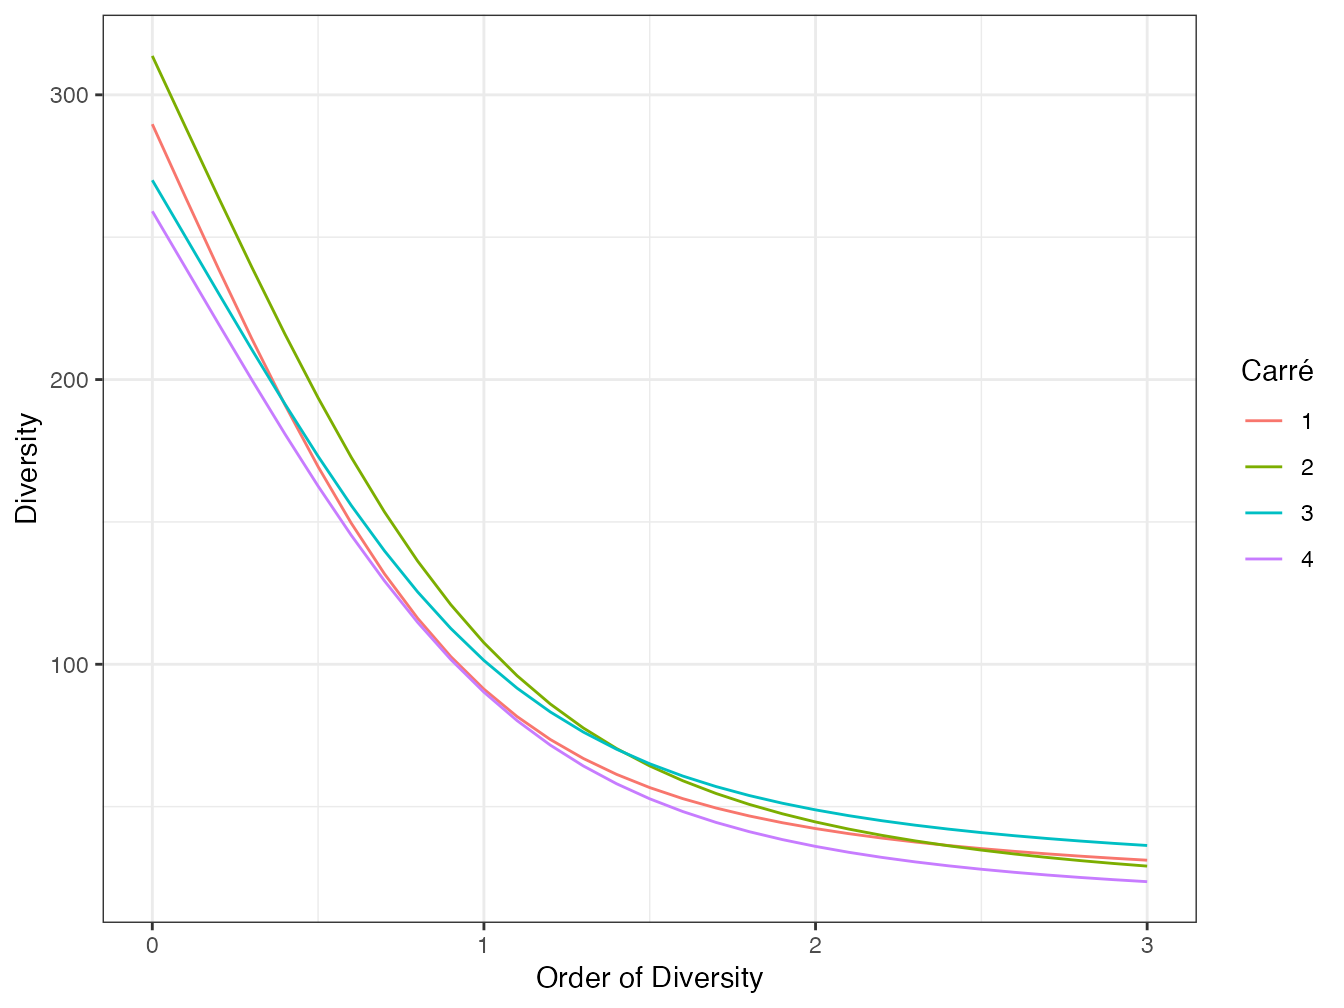
\includegraphics[width=0.8\linewidth]{MesuresBD_files/figure-latex/ProfilDivFig-1} 

}

\caption{Profils de diversité des quatre carrés de la parcelle 6 de Paracou. La correction du biais d'estimation est celle de Chao et Jost. Le carré 2 est plus divers que le carré 4, mais pas que les carrés 1 et 3, qui sont plus divers dans les grands ordres de diversité. Le profil de diversité est tracé ici jusqu'à l'ordre \(q = 3\).}\label{fig:ProfilDivFig}
\end{SCfigure}

\normalsize

Code R pour réaliser la figure \ref{fig:ProfilDivFig}:

\scriptsize

\begin{Shaded}
\begin{Highlighting}[]
\NormalTok{paracou\_6\_abd }\SpecialCharTok{\%\textgreater{}\%} 
  \CommentTok{\# Suppression de "subplot\_" dans les noms des carrés}
  \FunctionTok{mutate}\NormalTok{(}\AttributeTok{site =} \FunctionTok{str\_replace}\NormalTok{(.}\SpecialCharTok{$}\NormalTok{site, }\StringTok{"subplot\_"}\NormalTok{, }\StringTok{""}\NormalTok{)) }\SpecialCharTok{\%\textgreater{}\%} 
  \CommentTok{\# Profil}
  \FunctionTok{profile\_hill}\NormalTok{(}\AttributeTok{orders =} \FunctionTok{seq}\NormalTok{(}\DecValTok{0}\NormalTok{, }\DecValTok{3}\NormalTok{, .}\DecValTok{1}\NormalTok{), }\AttributeTok{estimator =} \StringTok{"ChaoJost"}\NormalTok{) }\SpecialCharTok{\%\textgreater{}\%}
  \FunctionTok{autoplot}\NormalTok{() }\SpecialCharTok{+}
  \FunctionTok{labs}\NormalTok{(}\AttributeTok{color =} \StringTok{"Carré"}\NormalTok{)}
\end{Highlighting}
\end{Shaded}

\normalsize

\textcite{Pallmann2012} ont développé un test statistique pour comparer la diversité de deux communautés pour plusieurs valeurs de \(q\) simultanément.

\textcite{Liu2006} nomment \emph{séparables} des communautés dont les profils ne se croisent pas.
Ils montrent que des communautés peuvent être séparables en selon un profil de diversité de \(^{q}\!D\) sans l'être forcément selon un profil de diversité de Hurlbert (section \ref{sec-Hurlbert}), et inversement.
Ils montrent que les communautés séparables selon un troisième type de profil, celui de la queue de distribution \autocite{Patil1982}, le sont dans tous les cas.
Le profil de la queue de distribution est construit en classant les espèces de la plus fréquente à la plus rare et en traçant la probabilité qu'un individu appartienne à une espèce plus rare que l'espèce en abscisse (figure \ref{fig:ProfilQueueFig}).



\scriptsize

\begin{SCfigure}

{\centering 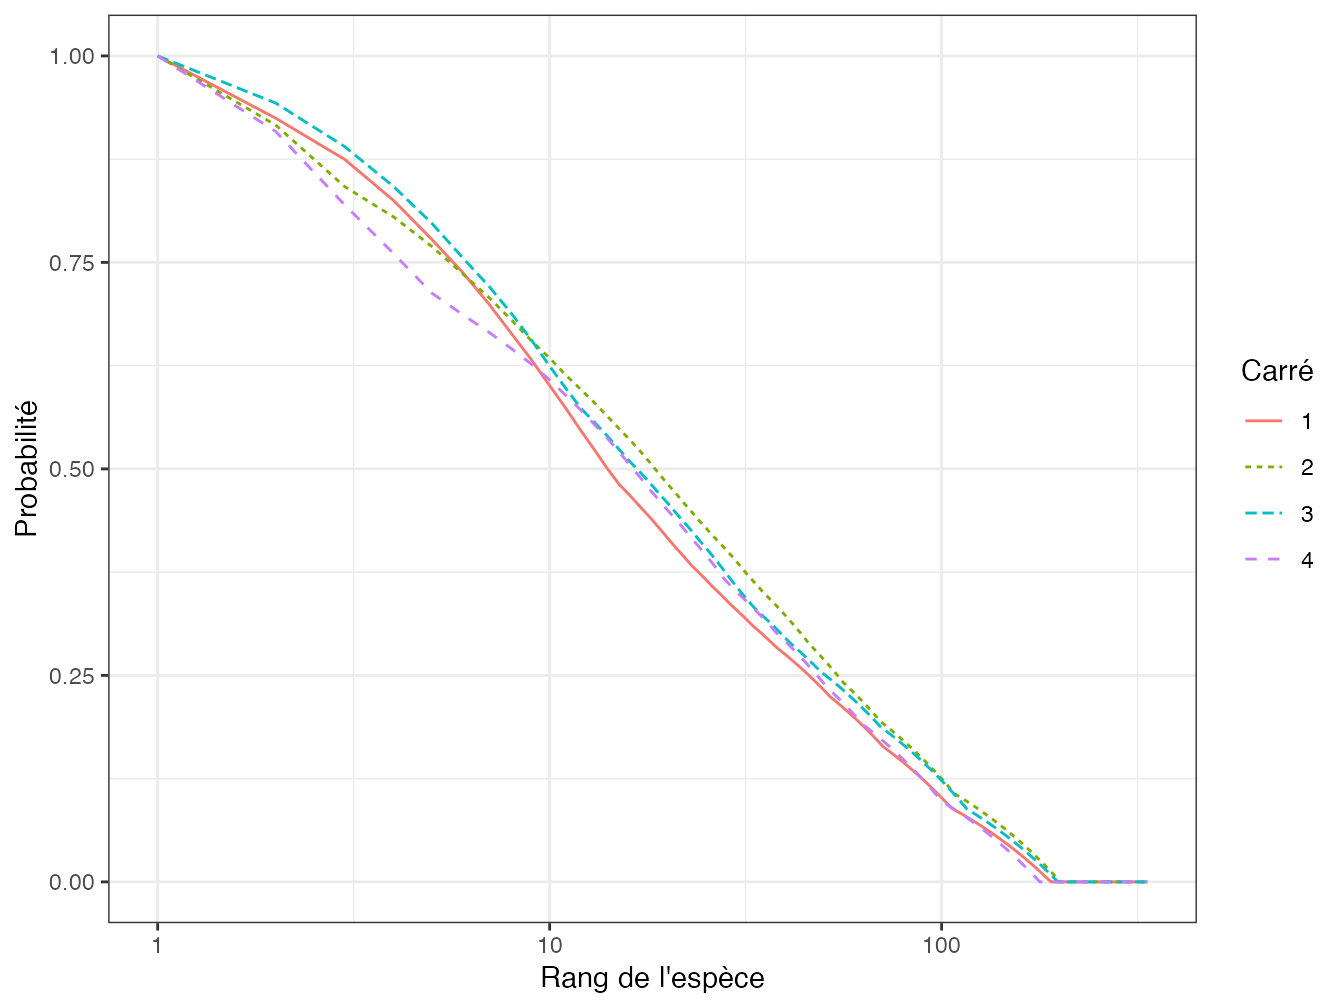
\includegraphics[width=0.8\linewidth]{MesuresBD_files/figure-latex/ProfilQueueFig-1} 

}

\caption{Profil de queue de distribution calculé pour les carrés de la parcelle 6 de Paracou. En abscisse: rang de l'espèce dans le classement de la plus fréquente à la plus rare; en ordonnée: probabilité qu'un individu de la communauté appartienne à une espèce plus rare. Les profils de queue de distribution se croisent d'autant plus tôt qu'ils se croisent pour de grands ordres de diversité dans la figure \ref{fig:ProfilDivFig}.}\label{fig:ProfilQueueFig}
\end{SCfigure}

\normalsize

Code R:

\scriptsize

\begin{Shaded}
\begin{Highlighting}[]
\NormalTok{paracou\_6\_abd }\SpecialCharTok{\%\textgreater{}\%}
  \CommentTok{\# Transformation en probabilités}
  \FunctionTok{as\_probabilities}\NormalTok{() }\SpecialCharTok{\%\textgreater{}\%}
  \CommentTok{\# Elimination des colonnes de description}
  \FunctionTok{as.matrix}\NormalTok{() }\SpecialCharTok{\%\textgreater{}\%} 
  \CommentTok{\# Tri des espèces par ordre croissant de probabilité}
  \FunctionTok{apply}\NormalTok{(}\AttributeTok{MARGIN =} \DecValTok{1}\NormalTok{, }\AttributeTok{FUN =}\NormalTok{ sort) }\SpecialCharTok{\%\textgreater{}\%} 
  \CommentTok{\# Cumul des probabilités. Attention: apply a transposé la matrice}
  \FunctionTok{apply}\NormalTok{(}\AttributeTok{MARGIN =} \DecValTok{2}\NormalTok{, }\AttributeTok{FUN =}\NormalTok{ cumsum) }\SpecialCharTok{\%\textgreater{}\%} 
  \CommentTok{\# Classement par valeurs décroissantes}
  \FunctionTok{apply}\NormalTok{(}\AttributeTok{MARGIN =} \DecValTok{2}\NormalTok{, }\AttributeTok{FUN =}\NormalTok{ rev) }\SpecialCharTok{\%\textgreater{}\%} 
  \CommentTok{\# Création d\textquotesingle{}un tibble pour le graphique}
  \FunctionTok{as\_tibble}\NormalTok{() }\SpecialCharTok{\%\textgreater{}\%} 
  \CommentTok{\# Nom des colonnes: 1 à 4}
  \FunctionTok{rename\_with}\NormalTok{(}\SpecialCharTok{\textasciitilde{}} \FunctionTok{str\_replace}\NormalTok{(., }\StringTok{"V"}\NormalTok{, }\StringTok{""}\NormalTok{)) }\SpecialCharTok{\%\textgreater{}\%} 
  \CommentTok{\# Ajout d\textquotesingle{}une colonne pour l\textquotesingle{}ordre}
  \FunctionTok{mutate}\NormalTok{(}\AttributeTok{rank =} \FunctionTok{seq\_len}\NormalTok{(}\FunctionTok{nrow}\NormalTok{(.))) }\SpecialCharTok{\%\textgreater{}\%} 
  \CommentTok{\# Création du graphique}
  \FunctionTok{pivot\_longer}\NormalTok{(}\AttributeTok{cols =} \SpecialCharTok{{-}}\NormalTok{rank) }\SpecialCharTok{\%\textgreater{}\%} 
  \FunctionTok{ggplot}\NormalTok{() }\SpecialCharTok{+}
    \FunctionTok{geom\_line}\NormalTok{(}\FunctionTok{aes}\NormalTok{(}\AttributeTok{x =}\NormalTok{ rank, }\AttributeTok{y =}\NormalTok{ value, }\AttributeTok{color =}\NormalTok{ name, }\AttributeTok{lty =}\NormalTok{ name)) }\SpecialCharTok{+}
    \FunctionTok{scale\_x\_log10}\NormalTok{() }\SpecialCharTok{+}
    \FunctionTok{labs}\NormalTok{(}
      \AttributeTok{x =} \StringTok{"Rang de l\textquotesingle{}espèce"}\NormalTok{, }
      \AttributeTok{y =} \StringTok{"Probabilité"}\NormalTok{, }
      \AttributeTok{color =} \StringTok{"Carré"}\NormalTok{,}
      \AttributeTok{lty =} \StringTok{"Carré"}
\NormalTok{    ) }
\end{Highlighting}
\end{Shaded}

\normalsize

Les coordonnées des points du profil sont définies par
\begin{equation}
  \label{eq:ProfilQueue}
  y(x) = \sum_{s=x+1}^{S}{p_{[s]}},\ x\in \{0, 1, \dots, S\}.
\end{equation}

\(p_{[s]}\) est la probabilité de l'espèce \(s\); les espèces sont classées par probabilité décroissante.

Ce profil est exhaustif (toutes les espèces sont représentées) alors que les autres profils de diversité ne sont représentés que pour un intervalle restreint du paramètre et qu'un croisement de courbes peut se produire au-delà.
En revanche, il ne prend pas en compte les espèces non observées.

\textcite{Fattorini1999} proposent un test pour comparer deux profils de queue de distribution à partir d'échantillonnages multiples (nécessaires pour évaluer la variance de chacune des probabilités) mais qui néglige les espèces non observées.


% Bibliography
%%%%%%%%%%%%%%%%%%%%%%%%%%%%%%%%%%%%%%%%%%%%%%%%%%%%%%%%%%

\backmatter
\SmallMargins

\twocolumn
\renewcommand*{\bibfont}{\scriptsize}
\printbibliography
\onecolumn


% Tables (of tables, of figures)
%%%%%%%%%%%%%%%%%%%%%%%%%%%%%%%%%%%%%%%%%%%%%%%%%%%%%%%%%%




% After-body (LaTeX code inclusion)
%%%%%%%%%%%%%%%%%%%%%%%%%%%%%%%%%%%%%%%%%%%%%%%%%%%%%%%%%%




% Back cover
%%%%%%%%%%%%%%%%%%%%%%%%%%%%%%%%%%%%%%%%%%%%%%%%%%%%%%%%%%%

% Even page, small margins, no running head, no page number.
\evenpage
\SmallMargins
\thispagestyle{empty}

\begin{normalsize}

\begin{description}

\selectlanguage{french}
\item[Résumé]
La biodiversité peut être mesurée de nombreuses façons.

La dualité entropie-diversité fournit un cadre clair et rigoureux pour le faire.
L'entropie est la surprise moyenne fournie par les individus d'une communauté.
Le choix de la fonction d'information qui mesure cette surprise à partir des probabilités d'occurence des espèces (ou d'autres catégories) permet de définir les mesures de diversités neutres, fonctionnelles ou phylogénétique présentées ici.
L'entropie est transformée en diversité au sens strict par une fonction croissante (l'exponentielle déformée), ce qui simplifie son interprétation en tant que nombre équivalent d'espèces.

L'entropie phylogénétique généralise les indices de diversité classique, intègre si nécessaire la distance entre espèces, peut être écomposée et corrigée des biais d'estimation.
Sa transformation en diversité au sens strict permet d'interpréter les valeurs sous une forme unique : un nombre équivalent d'espèces et un nombre équivalent de communautés.
La diversité de Leinster et Cobbold généralise à son tour la diversité phylogénétique et permet d'autres définitions de la distance entre espèces.
Le paramétrage des mesures (l'ordre de la diversité) permet de donner plus ou moins d'importance aux espèces rares et de tracer des profils de diversité.

La construction de ce cadre méthodologique est présentée en détail ainsi que plusieurs approches différentes, qui constituent l'état de l'art de la mesure de la biodiversité.
\item[]
.
~\\

\end{description}

\end{normalsize}

\vspace*{\fill}
\centering
\includegraphics[width=.3\textwidth]{images/logo}

\end{document}
